\documentclass[12pt,PhD,a4paper,twoside,pdftex]{muthesis}

% Define a boolean which says we are compiling my thesis
\newif\ifthesis
\thesistrue


%% General packages
%% ============================================================

% Add maths commands, symbols and fonts
\usepackage{amsmath}
\usepackage{amssymb}
\usepackage{amsfonts}
\usepackage{amsthm}
\usepackage{mathtools}

% Greek letters in text
\usepackage[euler]{textgreek}


\usepackage[linesnumbered]{algorithm2e}


\usepackage{url}                %Support for urls

% Allow hyperlinks to break over lines and turn off warning about it
\usepackage{silence}
\WarningFilter{hyperref}{You have enabled option `breaklinks'.}
\usepackage[hyphenbreaks]{breakurl}

% This stops the word count from complaining that it doesn't recognise
% packages. Note that the lack of a space in "%TC" is important!
%TC:ignore
\usepackage[colorlinks=true, % colour all links black (just using
            linkcolor=black, % colorlinks=false results in boxes around
            citecolor=black, % links)
            filecolor=black,
            urlcolor=black,
            breaklinks]{hyperref}
%TC:endignore

\usepackage{xspace} % command for fixing spaces after macros




% Language
% ============================================================
% Support for UTF8 input
\usepackage[utf8]{inputenc}

%% % Handle non-ascii fonts properly, see
%% % http://tex.stackexchange.com/questions/664/why-should-i-use-usepackaget1fontenc
%% \usepackage[T1]{fontenc}
%% % Seems to break searching so I'm not using it...

% Commonly recommend, not sure what it does...
\usepackage[UKenglish]{babel}



%% Page Layout
%% ============================================================
% Paragraphs use a vertical space rather than tabbing
\setlength{\parskip}{\medskipamount}
\setlength{\parindent}{0pt}
\usepackage[hang,flushmargin]{footmisc} % same for footnotes

% Adds a landscape enviroment
\usepackage{lscape}


%% Figure Tweaks
%% ============================================================
\usepackage[pdftex]{graphicx}   %Needed to include pictures

% positioning tweaks
\renewcommand{\topfraction}{0.85}
\renewcommand{\textfraction}{0.1}
\renewcommand{\floatpagefraction}{0.75}

% Italic captions
\usepackage[labelfont=it,textfont=it]{caption}

% package for \FloatBarrier which stops floats moving past it.
\usepackage{placeins}



%% Equations/maths
%% ============================================================
\numberwithin{equation}{chapter} % Number equations by "<chapter>.<number>".

%\usepackage{nath}
% % Prevent line break in the middle of maths except in extreme cases (increse numbers to make line breaking even more unlikely)
% \relpenalty=3000
% \binoppenalty=5000



%% Bibliograpy Tweaks
%% ============================================================

% biblatex setup
%TC:ignore
\usepackage[backend=biber,
  citestyle=numeric,
  firstinits=true, % Only print initials of first names
  isbn=false,
  doi=true,
  url=true, % for websites, see below for removing it from papers etc.
  % backref=true
]{biblatex}
%TC:endignore


% clear urls for papers, proceedings, books
\AtEveryBibitem{%
  \ifentrytype{article}{%
    \clearfield{url}%
    \clearfield{urldate}%
  }
  {}% no "else" operation
  %
  \ifentrytype{inproceedings}{%
    \clearfield{url}%
    \clearfield{urldate}%
  }
  {}% no "else" operation
  %
  \ifentrytype{book}{%
    \clearfield{url}%
    \clearfield{urldate}%
  }
  {}% no "else" operation
}

% Get rid of "In:" for journal articles
\renewbibmacro{in:}{%
  \ifentrytype{article}{}{\printtext{\bibstring{in}\intitlepunct}}}



% Add bibtex files
\addbibresource{mendeley_library.bib}

%% % A superscript ciation command
%% \DeclareCiteCommand{\supercite}[\mkbibsuperscript]
%%   {\iffieldundef{prenote}
%%      {}
%%      {\BibliographyWarning{Ignoring prenote argument}}%
%%    \iffieldundef{postnote}
%%      {}
%%      {\BibliographyWarning{Ignoring postnote argument}}}
%%   {\usebibmacro{citeindex}%
%%    \bibopenbracket\usebibmacro{cite}\bibclosebracket}
%%   {\supercitedelim}
%%   {}

%% % Use superscript cite instead of normal ones
%% \let\cite=\supercite



% Section etc. labelling
% ============================================================

% This goes last because apparently other packages can break cleveref

% \def\chapterautorefname{Chapter} % capitalise
% \def\sectionautorefname{Section} % capitalise
% \def\subsectionautorefname{Section} % capitalise, say section not subsection

%TC:ignore
\usepackage[sort&compress, % on multiple refs sort them and write as range
            capitalise, % Use Section not section etc.
            noabbrev, % Use Table not Tab. etc.
            nameinlink % Make the name (eg Section) part of the hyperlink
            ]{cleveref}

%TC:endignore

% Call subsections sections
\crefname{subsection}{Section}{Sections}
\Crefname{subsection}{Section}{Sections}

% just use (...) for equations
\crefformat{equation}{#2(#1)#3}
\crefrangeformat{equation}{#3(#1)#4--#5(#2)#6}
\crefmultiformat{equation}{(#2#1#3)}{ and~(#2#1#3)}{, (#2#1#3)}{ and~(#2#1#3)}

% Except for start of sentences where we need to say "Equations"
\Crefformat{equation}{Equation~#2(#1)#3}
\Crefrangeformat{equation}{Equations~#3(#1)#4--#5(#2)#6}
\Crefmultiformat{equation}{Equations~(#2#1#3)}{ and~(#2#1#3)}{, (#2#1#3)}{ and~(#2#1#3)}


% a reference for "this X"
\newcommand{\thisref}[1]{this \lcnamecref{#1}}
\newcommand{\Thisref}[1]{This \lcnamecref{#1}}



\setcounter{tocdepth}{1} % Set contents to only go down to section level


%% Flow charts
%% ============================================================
\usepackage{tikz} % Package for drawing flow charts
\usetikzlibrary{shapes,arrows}

\definecolor{paleblue}{RGB}{239,242,255}
\definecolor{solidblue}{RGB}{43,0,229}

% Define a rectangle shape and an arrow
\tikzstyle{block} = [rectangle, draw, fill=paleblue, thick,
    text width=4.3cm, text centered, rounded corners, minimum height=1cm]
\tikzstyle{line} = [draw, -]
\tikzstyle{arrow} = [draw, -latex']



% Define my commands
% ============================================================

%% Define new commands
%% ============================================================

%% General Latex commands
%% ------------------------------
% New way to define commands that allows multiple subscripts
\makeatletter
\newcommand\newsubcommand[3]{\newcommand#1{#2\sc@sub{#3}}}
\def\sc@sub#1{\def\sc@thesub{#1}\@ifnextchar_{\sc@mergesubs}{_{\sc@thesub}}}
\def\sc@mergesubs_#1{_{\sc@thesub#1}}


% define a macro to allow multiple references to be passed to \autoref
\newcommand\autorefs[1]{\@first@ref#1,@}
\def\@throw@dot#1.#2@{#1}% discard everything after the dot
\def\@set@refname#1{%    % set \@refname to autoefname+s using \getrefbykeydefault
  \edef\@tmp{\getrefbykeydefault{#1}{anchor}{}}%
  \def\@refname{\@nameuse{\expandafter\@throw@dot\@tmp.@autorefname}s}%
}
\def\@first@ref#1,#2{%
  \ifx#2@\autoref{#1}\let\@nextref\@gobble% only one ref, revert to normal \autoref
  \else%
  \@set@refname{#1}%  set \@refname to autoref name
  \@refname~\ref{#1}% add autoefname and first reference
  \let\@nextref\@next@ref% push processing to \@next@ref
  \fi%
  \@nextref#2%
}
\def\@next@ref#1,#2{%
  \ifx#2@ and~\ref{#1}\let\@nextref\@gobble% at end: print and+\ref and stop
  \else, \ref{#1}% print  ,+\ref and continue
  \fi%
  \@nextref#2%
}

\makeatother

%% % The LyX greyedout annotation environment
%% \usepackage{color}
%% \definecolor{note_fontcolor}{rgb}{0.80078125, 0.80078125, 0.80078125}
%% \newenvironment{lyxgreyedout}
%% {\textcolor{note_fontcolor}\bgroup\ignorespaces}
%% {\ignorespacesafterend\egroup}

% Latin
% ============================================================

% trailing slash is needed so that latex knows the final . is not the end
% of a sentence.

\newcommand{\ie}{\textit{i.e.}\ }
\newcommand{\cf}{\textit{c.f.}\ }
\newcommand{\eg}{\textit{e.g.}\ }
\newcommand{\etal}{\textit{et al.}\ }
\newcommand{\etc}{etc.\ }



%% General maths commands
%% ------------------------------
\newcommand{\pd}[2]{\frac{\partial #1}{\partial #2}} % partial deriv
\newcommand{\spd}[2]{\frac{\partial^2 #1}{\partial {#2}^2}} % 2nd partial deriv
\newcommand{\ddn}[1]{\pd{#1}{\nv}} % normal derivative
\newcommand{\vd}[2]{\frac{\delta #1}{\delta #2}} % variational derivative
\newcommand{\myvector}[1]{\mathbf{#1}}
\newcommand{\goesto}{\rightarrow}

\newcommand{\E}[1]{\times 10^{#1}} % powers of 10
\newcommand{\st}{\,|\,} % ``such that'' operator in sets (vertical line with spacing)

\newcommand{\ip}[2]{\left(#1,\, #2 \right)} % inner product
\newcommand{\ltip}[2]{\ip{#1}{#2}_{\ltwo}} % l2 inner product


% Norm and abs: better spacing than if done manually with |
\newcommand{\abs}[1]{\left|{#1} \right|}
\newcommand{\norm}[1]{\lVert #1 \rVert}
\newcommand{\ltnorm}[1]{\norm{#1}_{\ltwo}}

% rescaled time
\newcommand{\that}{\hat{t}}

% d for the end of integrals (e.g. dx) with correct spacing and non-italic
\renewcommand{\d}{{\; \text{d}}}
% standard integrals
\newcommand{\intd}[2][\magd]{{\int_{#1} #2 \d {#1}}}
\newcommand{\intb}[1]{\intd[\boundd]{#1}}

% Some vector functions
\newcommand{\gv}{{\myvector{g}}}
\newcommand{\fv}{{\myvector{f}}}
\newcommand{\pv}{{\myvector{p}}}


\newcommand{\ffv}[1]{{\myvector{f}\bigb{#1}}}
\newcommand{\gfv}[1]{{\myvector{g}\bigb{#1}}}


% Some vectors
\newcommand{\av}{{\myvector{a}}}
\newcommand{\bv}{{\myvector{b}}}
\newcommand{\cv}{{\myvector{c}}}
\newcommand{\sv}{{\myvector{s}}}
\newcommand{\kvec}{\myvector{k}}

\newcommand{\ev}{\myvector{\hat{e}}}
\newcommand{\nv}{\myvector{\hat{n}}}

\newcommand{\xv}{\myvector{x}}
\newcommand{\yv}{\myvector{y}}
\newcommand{\zv}{\myvector{z}}
\newcommand{\lv}{\myvector{l}}

\newcommand{\unitv}[1]{{\hat{\mathbf{#1}}}}
\newcommand{\iv}{\unitv{i}}
\newcommand{\jv}{\unitv{j}}
\newcommand{\kv}{\unitv{k}}
\newcommand{\unitz}{\unitv{z}}

% Matrices
\newcommand{\mymatrix}[1]{\mathrm{#1}}
\newcommand{\Pm}{\mymatrix{P}}
\newcommand{\Qm}{\mymatrix{Q}}
\newcommand{\Idm}{\mymatrix{I}}
\newcommand{\Am}{\mymatrix{A}}
\newcommand{\Gm}{\mymatrix{G}}
\newcommand{\Fm}{\mymatrix{F}}
\newcommand{\Mm}{\mymatrix{M}}
\newcommand{\Jm}{\mymatrix{J}}
\newcommand{\Km}{\mymatrix{K}}
\newcommand{\Jmca}{\mymatrix{J}_\text{ca}}
\newcommand{\Jmts}{\mymatrix{J}_\text{ts}}
\newcommand{\jts}{j_\text{ts}}

% Brackets
\newcommand{\bigb}[1]{{\left( #1 \right)}}
\newcommand{\bigs}[1]{{\left[ #1 \right]}}
\newcommand{\evalat}[1]{{\left|_{#1}\right.}}

% BEM
\newcommand{\bm}{{\mathbf{\Gm}}}
\newcommand{\tri}{\vartriangle}



% 3-component vector as a list of components
\newcommand{\threevec}[3]{\begin{pmatrix} #1 \\ #2 \\ #3 \end{pmatrix} }
\newcommand{\threevecdup}[1]{\threevec{#1}{#1}{#1}}


% Big O notation
\newcommand{\order}[1]{\text{O}(#1)}
\newcommand{\porder}[1]{\quad + \order{#1}} % with larger spacing

% Differential operators
\renewcommand{\div}{\nabla \cdot} % \div is normally division
\newcommand{\grad}{\nabla}
\newcommand{\curl}{\nabla \cross}
\newcommand{\lap}{\nabla^2}

\newcommand{\compdot}{\mathbin{:}}



%% Spaces, domains and geometrical labels
%% ------------------------------
% Domain labels used
\newcommand{\magd}{\Omega}
\newcommand{\boundd}{{\Gamma}}
\newcommand{\fulld}{{\real^d}}
\newcommand{\extd}{{\Omega^c}}

% Interior/exterior labels
\newcommand{\inte}{\text{int}}
\newcommand{\exte}{\text{ext}}

\newcommand{\real}{\mathbb{R}} % real numbers
\newcommand{\complex}{\mathbb{C}} % complex numbers
\newcommand{\integers}{\mathbb{Z}} % integer numbers

\newcommand{\sob}{\mathcal{H}} % Sobelov spaces
\newcommand{\ltwo}{L^2} %L2

\newcommand{\Dfs}{\mathcal{D}} % Set of functions that obey Dirichlet boundaries
\newcommand{\Neu}{{\scriptscriptstyle{\mathcal{N}}}} % Neumann


%% Magnetics
%% ------------------------------
% Define M, H, B vectors (i.e. bold)
\newcommand{\Mv}{\myvector{M}}
\newcommand{\Hv}{\myvector{H}}
\newcommand{\Bv}{\myvector{B}}


% polar coords
\newcommand{\ruv}{\myvector{\hat{r}}} % r unit vector
\newcommand{\phiv}{\myvector{\hat{\phi}}}
\newcommand{\thetav}{\myvector{\hat{\theta}}}
\newcommand{\rv}{\myvector{r}} % r vector


% Define some common types of H-field.
% if changing these beware of components of H which are not defined here.
\newsubcommand{\Heff}{\myvector{H}}{{\text{eff}}} %effective (total)
\newsubcommand{\Happ}{\myvector{H}}{{\text{ap}}} %applied
\newsubcommand{\Hms}{\myvector{H}}{\text{ms}} % magnetostatic/demag
\newsubcommand{\Hex}{\myvector{H}}{\text{ex}} % exchange
\newsubcommand{\Hca}{\myvector{H}}{\text{ca}} % crystalline ansiotropy
\newsubcommand{\Hthm}{\myvector{H}}{\text{th}} % thermal

\newcommand{\phim}{\phi} % magnetostatic potential
\newcommand{\phione}{u} % auxilary potential
\newcommand{\phitwo}{v} % other auxilary potential

% Normalised versions of the above fields (and M)
\newcommand{\mv}{\myvector{m}}
\newcommand{\hv}{\myvector{h}}
\newsubcommand{\heff}{\myvector{h}}{{\text{eff}}} %effective (total)
\newsubcommand{\happ}{\myvector{h}}{{\text{ap}}} %applied
\newsubcommand{\hms}{\myvector{h}}{\text{ms}} % magnetostatic/demag
\newsubcommand{\hex}{\myvector{h}}{\text{ex}} % exchange
\newsubcommand{\hca}{\myvector{h}}{\text{ca}} % crystalline ansiotropy
\newsubcommand{\hthm}{\myvector{h}}{\text{th}} % thermal
\newcommand{\nH}{H_{\mathbb{n}}} % A "magnitude" of H for normalisation

% Similarly for energies
\newsubcommand{\Eapp}{E}{{\text{ap}}} %applied
\newsubcommand{\Ems}{E}{\text{ms}} % magnetostatic/demag
\newsubcommand{\Eex}{E}{\text{ex}} % exchange
\newsubcommand{\Eca}{E}{\text{ca}} % crystalline ansiotropy
\newcommand{\e}{e} % total energy
\newsubcommand{\eapp}{e}{{\text{ap}}} %applied
\newsubcommand{\ems}{e}{\text{ms}} % magnetostatic/demag
\newsubcommand{\eex}{e}{\text{ex}} % exchange
\newsubcommand{\eca}{e}{\text{ca}} % crystalline ansiotropy
\newsubcommand{\ehop}{\e}{\hop} % total due to h operator fields


\newcommand{\nE}{E_{\mathbb{n}}} % A "magnitude" of energy for normalisation
\newcommand{\nA}{\mathbb{A}} % A "magnitude" of exchange const for normalisation
\newcommand{\nK}{\mathbb{K}} % A "magnitude" of anisotropy const for normalisation

% Magnetic constants
\newcommand{\Exchc}{A}
\newcommand{\Kone}{K_1}
\newcommand{\kone}{\mathcal{K}_1}
\newcommand{\dampc}{\alpha}
\newcommand{\dampeff}{\alpha_\text{eff}}
\newcommand{\gymagc}{{\abs{\gamma_{\text{\tiny{L}}}}}}


% SI magnetic units (Kronmuller2003)
\newcommand{\Mu}{{\text{Am}^{-1}}}
\newcommand{\Hu}{{\text{Am}^{-1}}}
\newcommand{\phiu}{{\text{A}}} % magnetic potentials
\newcommand{\Bu}{{\text{T}}}
\newcommand{\gymagu}{{\text{A}(\text{ms})^{-1}}}

% Define the LLG equation (in parts then all together)
\newcommand{\dMdt}{\pd{\Mv}{t}} % define dM/dt
\newcommand{\dmdt}{\pd{\mv}{t}}
\newcommand{\dMdn}{\pd{\Mv}{\nv}}
\newcommand{\dmdn}{\pd{\mv}{\nv}}

\newcommand{\MxH}{\Mv \times \Hv} % define M x H
\newcommand{\mxh}{\mv \times \hv}
\newcommand{\mxmxh}{\mv \left(\mv \times \hv \right)}
\newcommand{\MxdMdt}{\Mv \times \dMdt}
\newcommand{\mxdmdt}{\mv \times \dmdt}
\newcommand{\llg}{\dmdt = -(\mxh) + \dampc (\mxdmdt)}

%% Finite elements/numerical models
%% ------------------------------
% Define the test and shape functions
\newcommand{\tbf}{\varphi}
\newcommand{\tbfv}{\myvector{\varphi}}
\newcommand{\test}{v}
\newcommand{\testv}{\myvector{\test}}

\newcommand{\sbf}{\psi}
\newcommand{\ts}{{\mathcal{H}^1_h(\magd)}} % my test/shape fn space
\newcommand{\sk}{{\sbf_k}}
\newcommand{\tn}{{\tbf_\ndi}}

% Indices
\newcommand{\ndi}{n} % nodal index, not sure what to have it as...
\newcommand{\eli}{e} % element index
\newcommand{\tl}{l} % time-step index

% Green's functions - general form and main parts of 2/3D Green's functions for the laplacian operator
\newcommand{\Green}[1][]{G(\xv_{#1},\yv)}
\newcommand{\Gtwod}[1][]{\ln \abs{\xv_{#1} - \yv}}
\newcommand{\Gthreed}[1][]{\frac{1}{ \abs{\xv_{#1} - \yv}}}

% subscripts used
\newcommand{\ibasis}{{i}}
\newcommand{\ibasisb}{{j}}
\newcommand{\ibasisc}{{k}}

%% Time stepping
%% ------------------------------

% time step
\newcommand{\dtn}{\dtx{n}}
\newcommand{\dtx}[1]{\Delta_{#1}}

% "value step"
% Getting bold greek requires a hack because mathbf sees it as a "symbol"
% and so doesn't change it. This uses the direct TeX solution (from google!)
\newcommand{\dyn}{\dyx{n}}
\newcommand{\dyx}[1]{\mbox{\boldmath$\delta$}_{#1}}

% Denote various time steppers
\newcommand{\AB}{\text{AB}} % Adams-Bashforth 2
\newcommand{\imr}{\text{IMR}} % Implicit midpoint
\newcommand{\tr}{\text{TR}}
\newcommand{\bdf}{\text{BDF2}}
\newcommand{\FE}{\text{FE}} % Forward Euler (like)
\newcommand{\ebdf}{\text{eBDF3}}

% Local truncation errors
\newcommand{\lte}{T_n}

% Tol
\newcommand{\toltt}{\epsilon_{\dtx{}}}

% Newton's method
% ============================================================

% tol
\newcommand{\newtontol}{\epsilon_{\text{N}}}


% Operators
% ============================================================
\usepackage{mathrsfs}
\newcommand{\myop}[1]{\mathscr{#1}}
\newcommand{\hop}{\myop{H}}
\newcommand{\hmsop}{\myop{H}_{\text{ms}}}
\newcommand{\aop}{\myop{A}}
\newcommand{\bop}{\myop{B}}
\newcommand{\cop}{\myop{C}}
\newcommand{\lop}{\myop{L}}
\DeclareMathOperator{\realp}{real}

% Fractions
% ============================================================

%% Nice one line fractions
\usepackage{xfrac}
\usepackage[ugly]{nicefrac}

\newcommand{\half}{\nicefrac{1}{2}}


% Some typewritter text
% ============================================================

% Make sure it's not italic or anything as well as being tt, because it
% looks different (and stupid). \xspace makes sure there is a space
% afterwards at the correct times without having to explicitly write the
% empty argument (i.e. \toltt{}). It can be suppressed by writing the empty
% argument.
% \newcommand{\toltt}{{\textrm{\textup{\texttt{tol}}}\xspace}}
%% Didn't want this anyway in the end


% Stuff needed for galerkin
% ============================================================
\newcommand{\skewop}{\text{\Large{$\Lambda$}}}
\newcommand{\skewm}[1]{\skewop\left[ #1 \right]}
\newcommand{\crossop}[2]{\skewm{ #1 } \cdot \left( #2 \right)}

\newcommand*\circled[1]{\tikz[baseline=(char.base)]{
    \node[shape=circle,draw,inner sep=1pt] (char) {#1};}}
\newcommand{\mxex}{I}
\newcommand{\mxmxex}{J}

\newcommand{\intp}[1]{\sum_\ibasisc \sk #1_\ibasisc}
\newcommand{\intpb}[1]{\left( \intp{#1} \right)}
\newsubcommand{\hs}{\hv}{\text{s}}

\newcommand{\ik}{\ibasisc}

% residuals
\newsubcommand{\rex}{\myvector{r}}{\text{ex}}
\newsubcommand{\rexh}{\myvector{r}}{\text{ex,h}}
\newsubcommand{\rll}{\myvector{r}}{\text{ll}}
\newcommand{\rllg}{\rv}
\newcommand{\rphi}{s}



% Notation for midpoint method stuff
% ============================================================

% t at midpoint
\newcommand{\thfx}[1]{t_{#1+\half}}
\newcommand{\thf}{\thfx{n}}

% exact y of t at midpoint
\newcommand{\yvhfx}[2]{\yv#1(\thfx{#2})}
\newcommand{\yvhf}[1][]{\yvhfx{#1}{n}}

% midpoint approximation to y
\newcommand{\yvmx}[1]{\yv_{#1+\half}}
\newcommand{\yvm}{\yvmx{n}}


% df/dy matrix
\newcommand{\dfdy}{F}
\newcommand{\dfdyhfx}[1]{\dfdy_{#1+\half}}
\newcommand{\dfdyhf}{\dfdyhfx{n}}

% error due to midpoint approx
\newcommand{\ymiderr}{a_n}

% full expressions for midpoint values
\newcommand{\mpm}{\frac{\mv_{n+1} + \mv_n}{2}}
\newcommand{\mpt}{\frac{t_n + t_{n+1}}{2}}
\newcommand{\mpdmdt}{\frac{\mv_{n+1} - \mv_n}{\dtn}}
\newcommand{\mphop}{\hop \left[ \mpm \right]}
\newcommand{\mphapp}{\happ \left(\mpt \right)}


% Commands from intermag paper 
% ============================================================

\newcommand{\dash}{\text{-}}
\newcommand{\dtinitial}{\dtx{\text{init}}}
\newcommand{\dtmax}{\dtx{\text{max}}}
\newcommand{\zerov}{\mathbf{0}}
\newcommand{\mvtemp}{\tilde{\mv}}


% Paper/thesis commands
% ============================================================

\ifthesis
\newcommand{\secpaper}{Section}
\else
\newcommand{\secpaper}{paper}
\fi


%%% Local Variables:
%%% mode: latex
%%% TeX-master: "main"
%%% End:



%% Beginning of main document
%% =============================================================

% Include only some sections while working on them, remove before final
%\includeonly{first_year_progress}

\title{Numerical methods for micromagnetics}
\author{David Shepherd}
\principaladviser{Jim Miles\\
  Milan Mihajlovi\'{c}\\
  Matthias Heil}
% \submitdate{29th September 2014}

% \date{30 March 2012}


\begin{document}

% muthesis stuff:
%%%%%%%%%%

% disable some useless pages
% \figurespagefalse
\tablespagefalse
% \copyrightfalse

\beforeabstract
\abstracttitle
Micromagnetics is a continuum mechanics theory of magnetic materials widely used in industry and academia.
In this thesis we describe a complete numerical method, with a number of novel components, for the computational solution of dynamic micromagnetic problems by solving the Landau-Lifshitz-Gilbert  (LLG) equation.
In particular we focus on the use of the implicit midpoint rule (IMR), a time integration scheme which when applied to the LLG conserves magnetisation length and, in the case of zero damping, the energy.
We use the finite element method (FEM) for spatial discretisation, and use nodal quadrature schemes to retain the conservation properties of IMR despite the weak-form approach.

We introduce a novel, generally applicable adaptive time step selection algorithm for the IMR.
We show that our scheme selects error-appropriate time steps for a variety of problems and that it retains the conservation of magnetisation length and conservation of energy properties of the fixed step IMR.
We also show how these conservation properties can be extended to the PDE case using finite elements with a nodal quadrature scheme.

We demonstrate how hybrid FEM/BEM magnetostatic calculations can be coupled to the LLG equation in a monolithic manner.
This allows the coupled solver to maintain all properties of the standard time integration scheme, in particular the energy conservation property of IMR and the solution converged to in the stochastic case.
We also develop a preconditioned Krylov solver for the coupled system which can efficiently solve the monolithic system given an effective preconditioner for the decoupled LLG system.

Finally we investigate the effect of the spatial discretisation on the comparative effectiveness of implicit and explicit time integration schemes (\ie the stiffness).
We find that explicit methods are more efficient for simple problems, but for the fine spatial discretisations, required in a number of more complex cases, implicit schemes become much more efficient.

\afterabstract

\prefacesection{Acknowledgements}
I would like to thank...

supervisors

Ray

Sylwia

family

NEST group

\oomph group

and all the people I met....

epsrc funding

\afterpreface

%%%%%%%%%% % end of muthesis stuff



\chapter{Introduction}
\label{sec:introduction}

In this thesis we study numerical techniques for the modelling of ferromagnetic materials.
In ferromagnetic materials, referred to in this thesis as simply ``magnetic materials'', exchange coupling between nearby spins causes the emergence of spontaneous magnetisation.
Some magnetic materials have preferred magnetisation directions (anisotropy), for example due to the crystal lattice structure, and in such materials systems with two stable states can be obtained.
The system can be switched between these states by the application of a magnetic field, which can be easily generated using pulses of electrical current.
These states can be extremely stable, having average lifetimes of decades at room temperature even for extremely small volumes of material.
Such materials have many technological applications, one major application is in the area of data storage.

In current hard disk drives collections of nanometre-sized grains of anisotropic magnetic material are magnetised using a write head (an electromagnet) in order to store bits of data.
The data can be read by magnetoresistive sensors, which change their resistance based on the magnetic field.
Such sensors can be extremely sensitive and extremely small, allowing them be very close to the bits and to obtain good signal-to-noise ratios despite the small size of the bits.

Another application area where ferromagnetic materials show great promise is in random access memory (RAM), \ie short term data storage for computers.
The current standard RAM technology (dynamic RAM or DRAM) is based on charging capacitors.
These capacitors leak charge fairly rapidly, resulting in data lifetimes on the order of milliseconds.
Hence they must be continually refreshed and can require significant power usage to retain data.
A widely proposed alternative is MRAM (magnetoresistive RAM) which uses arrays of nano-sized regions of magnetic material to store data and in-place magnetoresistive sensors to allow random-access reads.
The vastly longer data lifetimes allowed by the use of magnetic materials results in greatly reduced standby power usage by removing the requirement for continual refreshing.
Also computers could be easily put into a completely powered-off hibernation state without writing data to disk.
Historically there have been issues with random-access writes in MRAM: moving write heads (as used in hard drives) cannot be used because the time to move the head to the correct location is far too long, and in-place generation of the required magnetic fields requires large currents.
However recent developments in spin-torque-transfer, where spin-polarised currents are used to directly apply a torque to the magnetisation of a ferromagnet, offer a solution to these difficulties.
Spin torque transfer MRAM (ST-MRAM) has recently been commercialised by Everspin Technologies \cite{everspin} and is beginning to make its way into products.
Due to the combination of non-volatility, high density, random-access, and low read/write times such ST-MRAM is a candidate for a so-called ``universal memory'', where all data is stored a RAM-like memory eliminating long access times.


It is extremely desirable to be able to accurately model the behaviour of magnetic materials for both research and device design purposes.
However the use of models based on quantum mechanics (such as density functional theory) to predict the behaviour of magnetic systems is extremely computationally expensive due to the length scales required.
Instead a theory known as micromagnetics is typically employed \cite{Aharoni1996}.
In micromagnetics a continuum approximation of the ferromagnet's magnetisation is used -- it is  assumed that everything can be modelled using continuous functions of space and time (\ie the contribution due to individual atoms is averaged out).
This is a good approximation for many cases because of the smoothing effect of the ferromagnetic exchange effect.
Additionally a semi-classical approach is used: the various important quantum mechanical effects are approximated by classical representations.
The result of these approximations is a powerful framework for theoretical and computational predictions of the behaviour of magnetic materials.

Micromagnetic models can be broadly split into two categories: energy based models and dynamic models.
Energy based models aim to find stable minimum energy states for the system whereas
dynamic models simulate the evolution of the magnetisation over time.
Dynamic models may be favourable even when there are no time-dependent effects because standard energy based models are unable to distinguish which of the various stable states will be the final state of the system.
Dynamic micromagnetic models require the solution of a differential equation, known as the Landau-Lifshitz-Gilbert equation (LLG).
Depending on the physical system modelled the LLG may be an ordinary, partial or stochastic differential equation.
The very closely related Landau–Lifshitz–Slonczewski equation can be used to model magnetisation dynamics when spin-torque-transfer effects are included.


In this thesis we study numerical methods with the final goal of finding more reliable and efficient methods for dynamic micromagnetics simulations.
In particular we focus on methods which improve the efficiency of so-called ``geometric integration'' schemes.
Geometric integration schemes are numerical methods which are able to retain important \emph{qualitative} properties of a differential equation in an approximate solution.
In other areas of computational physics such methods have been shown to greatly reduce the overall accumulation of numerical errors \cite[77]{Iserles2009}.
This allows either more accurate results at the same computational cost, or the use of coarser approximations (reducing the computational cost) without loss of accuracy.
In particular we focus mainly on a widely known time integration scheme with geometric integration properties when applied to dynamic micromagnetics calculations: the implicit midpoint rule.



\section{Contents of thesis}

The first two chapters, \cref{sec:cont-micromag,sec:numer-meth-micr}, comprise a basic introduction to micromagnetic models and the numerical methods commonly used.
In particular \cref{sec:time-discretisation} contains a detailed description of the properties of a selection of time integration schemes.
\Cref{sec:galerk-meth-llg} gives a more detailed introduction to the finite element method, including a description of how it can be applied to dynamic micromagnetics simulations.
The chapter ends with a discussion of how the basic finite element method can be extended to retain the geometric integration properties of the implicit midpoint rule.
\Cref{sec:hybr-finit-elem} introduces the hybrid FEM/BEM method, a widely used technique for the accurate calculation of magnetostatic fields.

The later chapters contain the research contribution of this thesis.
\Cref{sec:solution-strategies} describes efficient techniques for the solution of the coupled systems resulting from the use of FEM/BEM magnetostatics calculations in an LLG-based dynamic model.
In particular we introduce techniques which reduce the development of an efficient solver for such a monolithically coupled model to the development of an effective preconditioner for the LLG alone.
Such a coupling strategy is required to retain the geometric integration properties of the implicit midpoint rule, and may also be useful in the time integration of the stochastic LLG.

In \cref{sec:adaptive-imr} we introduce a novel adaptive time step selection algorithm for the implicit midpoint rule.
This algorithm is not specific to the LLG, and to our knowledge is the first such algorithm.
The same chapter also contains numerous numerical experiments demonstrating the selection of appropriate time steps for a number of ordinary differential equations (ODEs), and demonstrating the geometric integration properties when applied to an ODE form of the LLG.

In \cref{cha:numer-experiments} we present a number of numerical experiments using combinations of the methods developed in this thesis.
The methods are validated against a number of examples: a wave-like problem with an analytical solution, relaxation under a non-uniform field and the \mumag standard problem \#4.
Additionally the convergence and geometric integration properties of a variety of time integration schemes are compared for problems.

Finally in \cref{cha:stiffn-llg-equat} the comparative efficiency of two classes of time integration schemes (implicit and explicit) are compared for an example problem across a range of spatial discretisations.

\Cref{cha:analyt-solut-land} contains a description of two analytical solutions to the LLG equation which have proven very useful in the verification of our implementation.
The other appendices contain technical details of some derivations.


%%% Local Variables:
%%% mode: latex
%%% TeX-master: "main"
%%% End:

\section{Continuous Micromagnetics}
\label{sec:cont-micromag}

In this section we give an introduction to micromagnetics including a statement of the equations to be solved.

\subsection{Definitions}
We use S.I. units throughout unless otherwise specified. In particular normalised quantities are no longer in S.I. units.

We define $\Hv(\xv,t)$ to be the magnetic field at position $\xv$ and time $t$ in units of $\Hu$.

We define $\Mv(\xv,t)$ to be a vector field representing the expectation value of the magnetisation per unit volume averaged over a number of unit cells.\cite{Aharoni1996}
The units of $\Mv$ are $\Mu$, the length of $\Mv(\xv,t)$ is given by the saturation magnetisation $M_s$.
At zero temperature $M_s$ is a fixed parameter of the material but in finite temperature models $M_s$ may vary.

These quantities are related to the magnetic flux density $\Bv(\xv,t)$ (in units of $\Bu$) by
\begin{equation}
  \label{eq:37}
  \Bv(\xv,t) = \mu_0 \left( \Hv(\xv,t) + \Mv(\xv,t) \right),
\end{equation}
% \cite{Gilbert2004} says that this magnetisation is different - averaged over all material rather than over a few cells...
where $\mu_0$ is the magnetic constant (or permeability of free space).

In general we will not make dependencies on $\xv$ and $t$ explicit.

\subsection{Energy of a Magnetic Body}
\label{sec:energy-magnetic-body}

The effects that must be considered in a micromagnetic mode are: the magnetostatic self field, the exchange energy and the magnetocrystalline anisotropy energy. Also important is the external applied field due to magnetic bodies or electrical currents outside the modelled region. Other effects which are sometimes important include temperature (thermal effects) and magnetostriction energy (due to stretching or compressing the magnet).

We begin by providing a description of each of these effects and their contribution to the total energy density, $E$. We can get the effective fields given by these energies by taking
\begin{equation}
  \Hv = \dfrac{-1}{\mu_0 V_{\magd}} \dfrac{\delta E}{\delta \Mv},
\end{equation}
where $\delta$ indicates a variational derivative and $V_{\magd}$ is the volume of the magnetic domain. ??ds citation? Is this correct?

%% Energy and field expressions below are taken from Matteo Franchin's thesis.\cite{Franchin2009}\footnote{Note that due to the variety in unit systems, definitions of magnetisation and other choices it can be difficult to compare energy/effective field equations from different authors, in particular the location of factors of $\mu_0$.}

\subsubsection{Exchange Energy}

In a ferromagnetic material neighbouring magnetic moments prefer to align parallel to each other due to quantum mechanical effects. This can be well approximated by a classical expression for exchange energy:\cite{Aharoni1996}
\begin{equation}
  \label{eq:39}
  \Eex =  \frac{\Exchc}{M_s^2} \int_{\magd} (\nabla M_x)^2  + (\nabla M_y)^2  + (\nabla M_z)^2 \d \magd,
\end{equation}
where $A$ is the material dependant exchange constant which depends on the crystal structure and the strength of the exchange coupling between electrons in the material.

We write the vector Laplacian as $\nabla^2 \Mv = (\nabla^2 M_x,\nabla^2 M_y, \nabla^2 M_z )$. Then the exchange effective field is given by
\begin{equation}
  \label{eq:Hex}
  \Hex = \frac{2 \Exchc}{ \mu_0 M_s} \nabla^2 \Mv.
\end{equation}

\subsubsection{Magnetostatic Field}
\label{sec:magnetostatic-field}

Magnetic materials generate magnetic fields, which in turn affects the magnetic material. This type of field is also known as the demagnetising field since it tends to oppose the magnetisation of the body. The magnetostatic field, $\Hms$, can be calculated in two ways: an integral based method or a potential based method. These methods are discussed in Sections~\ref{sec:magstat-field-calc-inte} and \ref{sec:magstat-field-calc-pote} respectively.

Once the self field has been calculated the energy contribution due to it is given by
\begin{equation}
  \label{eq:41}
  \Ems =  \frac{-\mu_0}{2} \int_{\magd} \Mv \cdot \Hms \d \magd,
\end{equation}
where the factor of $\frac{1}{2}$ is to avoid double counting.

Similarly any external applied field gives an energy contribution of
\begin{equation}
  \label{eq:42}
  \Eapp = - \mu_0 \int_{\magd} \Mv \cdot \Happ \d \magd.
\end{equation}

\subsubsection{Magnetocrystalline Anisotropy}
\label{sec:magn-anis}

Many magnetic materials have a preferred direction (or directions) of magnetisation due to their crystal structure. This is known as magnetocrystalline anisotropy. The equation for the magnetocrystalline anisotropy energy depends on the crystal structure of the material.

A detailed description of the many varieties of magnetocrystalline anisotropy is beyond the scope of this report but can be found in various textbooks on magnetic materials.\cite{Coey2010}\cite{Aharoni1996} However, since the anisotropy term is always a simple function of $\Mv$ it is not important for the implementation of a numerical model which type is used. Hence we give only the most useful case: in magnetic data recording we are interested in materials with a single \emph{easy axis} either in the plane of the disk or perpendicular to it since magnetisation is most stable in these types of material. The first order approximation for the free energy contribution for a perpendicular uniaxial material is given by
\begin{equation}
  \Eca = K_u \int_\magd 1 - \left( \mv \cdot \ev \right)^2 \d \magd,
  \label{eq:36}
\end{equation}
where $\ev$ is the easy axis and $K_u$ is the (material dependant) first order anisotropy energy density coefficient.\footnote{It is possible to define many different forms for this energy. Be warned that the choice of definition changes the meaning of $K_u$!} The first order approximation is valid when the anisotropy energy density coefficients are such that $K_u = K_1 >> K_2$, which is the case in most materials.\cite{Kronmuller2003} The effective field corresponding to this case is
\begin{equation}
  \Hca = \frac{2 K_u}{\mu_0 M_s} \left( \mv \cdot \ev \right) \; \ev.
  \label{eq:Hca}
\end{equation}


\subsection{Core Models}
??ds before energy/fields?

The general aim of a micromagnetic model is to predict the behaviour of a magnetic body under a variety of conditions. This can either be done by finding the minimum energy of the body or by modelling the dynamics of the magnetisation.

\begin{figure}[ht!]
  \centering
  \begin{tikzpicture}[level 1/.style={sibling distance=6cm},
    level 2/.style={sibling distance=5cm}]
    \node[block] {\textbf{Micromagnetics models}}
    child {node[block] {Energy Based}}
    child {node[block] {Dynamic}
      child {node[block] {Landau--Lifshitz Equation}}
      child {node[block] {Landau--Lifshitz--Gilbert Equation}}
    };
  \end{tikzpicture}
  \caption{Possible approaches of a standard numerical micromagnetic model.}
  \label{fig:types-micromag-model}
\end{figure}


\subsubsection{Energy Based Micromagnetics}
\label{sec:energy-based-micr}

Energy based methods find an equilibrium state of the magnetic system by finding the minimum energy with respect to variation of $\Mv$. For example Fredkin and Koehler used a finite element energy minimisation method.\cite{Koehler1992} Energy based methods require less computational effort than dynamic methods. However they cannot give any information about the time evolution of a system.\cite{Fidler2000} This is an important problem in many areas: for example in magnetic data storage the time taken to reverse the magnetisation of a bit is of key interest.

% could include more details on how to search for minima.

\subsubsection{Dynamic Micromagnetics}
\label{sec:land-lifsch-gilb}

Dynamic micromagnetic methods model the time evolution of the magnetisation, for given effective field, as a differential equation. Starting with the quantum mechanical angular momentum of an electron, and converting from a single spin a continuous magnetisation gives\cite{Kronmuller2003}
\begin{equation}
  \label{eq:38}
  \dMdt = - \gymagc \Mv \times \Hv,
\end{equation}
where $\Hv$ is the total effective field
\begin{equation}
  \Hv = \Happ + \Hca + \Hex + \Hms.
  \label{eq:Heff}
\end{equation}
Equation~\eqref{eq:38} represents the procession of the magnetisation about the effective field, as shown in Figure~\ref{fig:LLG-terms}. Other effective fields can be added to equation~\eqref{eq:Heff} to model other physical effects such as finite temperature or magnetostriction.

However equation~\eqref{eq:38} implies that the precession motion is undamped, \ie no energy is lost and the magnetisation continues to precess forever. This is obviously not the case so an empirical damping term is added:
\begin{equation}
  \label{eq:LL}
  \dMdt = - \gymagc \Mv \times \Hv - \frac{\dampc \gymagc}{M_s} \Big( \Mv \times (\Mv \times \Hv) \Big),
\end{equation}
where $\dampc$ is an experimentally determined material parameter related to the strength of the damping. Equation~\eqref{eq:LL} is referred to as the Landau--Lifshitz.\cite{Landau1935} The effects of the precession and damping terms are shown in Figure~\ref{fig:LLG-terms}.

\begin{figure}[ht!]
  \centering
  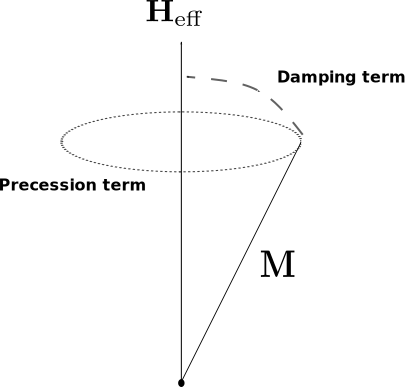
\includegraphics[width=0.6\textwidth]{./images/LLG-terms}
  \caption{The effects of the precession and damping terms in the Landau--Lifshitz and Landau--Lifshitz--Gilbert equations on the magnetisation direction, $\Mv$, of a single magnetic moment with a constant effective field
.}
  \label{fig:LLG-terms}
\end{figure}

However, there are still problems with this equation: for large damping the overall speed of the
motion increases without any increase in the precession speed. Hence the damping dominates and the switching time increases as damping is increased which is physically incorrect.\cite{Mallinson1987} There is another form of equation~\eqref{eq:LL} due to Gilbert\cite{Gilbert2004}, called the Landau--Lifshitz--Gilbert equation, which does not suffer from this problem
\begin{equation}
  \label{eq:Gilbert}
  \dMdt = - \gymagc \Mv \times \Hv + \frac{\dampc}{M_s} (\Mv \times \dMdt),
\end{equation}
where $\dampc \neq \dampc_L$. Equation~\eqref{eq:Gilbert} can be rearranged into the same form as equation~\eqref{eq:LL}, giving
\begin{equation}
  \label{eq:LLG}
  %\tag{LLG}
  \dMdt = \frac{-\gymagc}{1 + \dampc^2} \Big[ (\MxH) + \frac{\dampc}{M_s} \Big(\Mv \times (\MxH) \Big) \Big].
\end{equation}

Equations~\eqref{eq:LL}, \eqref{eq:Gilbert} and \eqref{eq:LLG} link the unknown magnetisation vector as a function of time $\Mv(t)$ with the effective field $\Hv$. To determine $\Mv$ at an arbitrary time $t \neq 0$ we need to integrate one of the above equations with respect to time. This is usually done numerically by employing a time discretisation method as discussed in Section~\ref{sec:time-discretisation}.

Note that there is no spatial dependence directly contained in equations~\eqref{eq:LL}, \eqref{eq:Gilbert} and \eqref{eq:LLG}. However the exchange effective field and magnetostatic field do contain spatial dependence, so usually the final equation to be solved after all substitutions really is a partial differential equation.

Examples of currently available micromagnetic models include the \texttt{OOMMF}\cite{oommf-website} and \texttt{nmag}\cite{Fischbacher2007} packages, which both use the dynamic method exclusively, along with \texttt{magpar}\cite{Scholz2003} and \texttt{FEMME}\cite{suessco-website} which can use either dynamic or energy based methods.


% \subsection{Accounting for Thermal Effects}
% \label{sec:thermal-effects}
% ??ds put in from other file when ready




% \subsubsection{Magnetostrictive Effects}
% \label{sec:magstric-effects}
% probably will never include this...


% \subsection{Limitations of Micromagnetics}
% ??ds put in from another file when ready


%%% Local Variables:
%%% mode: latex
%%% TeX-master: "./main"
%%% End:

\chapter{Numerical Methods for Dynamic Micromagnetic Modelling}
\chaptermark{General numerical methods}
\label{sec:numer-meth-micr}

\section{Introduction}

In \thisref{sec:numer-meth-micr} we give an overview of numerical methods that have previously been used in dynamic micromagnetic calculations.
These calculations involve solving some form of the LLG equation \cref{eq:LLG} with effective fields determined by energy derivatives as discussed in \cref{sec:cont-micromag}.
These systems of partial differential equations (PDEs) can only be solved analytically in a few simple cases \cite{Aharoni1996}, so numerical solution methods are almost always necessary.


\subsection{Components of a numerical method for solving PDEs}

Many numerical methods for solving non-linear PDEs, such as the LLG \cref{eq:LLG}, can be thought of as a combination of various component methods, each of which handles a different part of the conversion from a continuous PDE into an algorithm which can be performed by a computer\footnote{Technically proofs of convergence etc. should be carried out for every different combination of component methods \cite[382]{Iserles2009}; in practice surprises seem to be rare, at least within micromagnetics.}.

The essential components of a numerical method for solving time-dependent PDE problems are:
\begin{itemize}
\item Spatial discretisation: convert spatial derivatives into algebraic relationships, typically between discrete points in space, \eg finite elements, finite differences, macrospin models.
\item Time discretisation (a.k.a. time integration): convert time derivatives into algebraic relationships, again typically between points in time, \eg Runge-Kutta methods, backwards difference formulae.
\end{itemize}
For some choices of time and space discretisations additional component methods are needed:
\begin{itemize}
\item Linearisation procedure: Solve a system of non-linear algebraic equations, often by an iterative procedure which requires the solution of a sequence of systems of linear algebraic equations, \eg Newton-Raphson method, Picard/fixed-point iteration.
\item Linear solver: solve a system of linear algebraic equations, \eg LU decomposition, Krylov solvers, multigrid methods.
\end{itemize}

Additionally in micromagnetic modelling the calculation of the magnetostatic field is required.
If the integral form of the magnetostatic field, given in \cref{eq:Hmsint}, is used then an additional integral evaluation method is needed to handle it.
Alternatively, if the equivalent potential formulation, given in \cref{eq:Hms,eq:cont-phi-bound}, is used then the magnetostatic field calculation simply requires solving additional PDEs, although there are some issues with the application of the boundary condition at infinity which are discussed in \cref{sec:magstat-field-calc-pote}.


\subsection{Desirable properties of a numerical method}
\label{sec:desir-prop-numer}

Ideally all numerical methods would run quickly on cheap hardware and with sufficient accuracy.
Unfortunately this is not the case in general and we are forced to make trade-offs.
In \thisref{sec:desir-prop-numer} we roughly describe some \emph{ideal} properties of a numerical method (although obtaining all of these properties in a single method is almost certainly impossible).

The accuracy of a simulation is generally proportional to the ``fineness''  of the discretisations used (\ie the number of points used in the approximation), but increasing the fineness also increases the computation time.
However, careful choice of algorithms can improve the accuracy at no additional cost or improve the speed with no loss of accuracy.
The following properties of methods are important in this respect:
\begin{itemize}
\item The discretisation fineness in time should be dictated only by what is needed to accurately resolve the physics and not by numerical properties of the discretisation.
  In particular improved spatial fineness should not require improved time fineness.

\item The optimal fineness in both time and space should be determined automatically, and should be allowed to vary as needed.
  This allows us to get the best ``value'' for our computational effort when increasing the fineness of the discretisation.

\item The computation time should increase as little as possible as fineness in space or time increases.
  The minimum increase is linear scaling ($\order{N}$, where $N$ is the number of discrete points involved) because we always have to do \emph{something} with each value.
  Attaining this property for spatial discretisation usually impacts the choice of linear solver and/or magnetostatic calculation: many methods do not scale this well.

\item The method should be able to handle non-trivial geometries without extortionate computational cost.
\end{itemize}

Additionally we would like our algorithms to be robust, that is they should reliably be able to give a correct answer no matter what parameters are used (up to any tolerances specified).
In other words there should be few edge cases or ``interesting'' surprises when applying the method to various physical problems.
Some important properties which improve robustness are:
\begin{itemize}
\item The method should obey any qualitative physical properties of the continuous equation.

\item Mathematical evidence that all parts of the method will ``work'' on any well defined problem (\eg proofs of convergence, etc.).

\item The numerical method should automatically detect difficulties and apply the required effort to obtain the correct answer.
\end{itemize}


In addition to these properties there are a few practical considerations.
The method should be reasonably simple: people need to understand a method before they can implement it, and even users need a surface level understanding.
Finally the method should be as general as possible to reduce implementation effort and to simplify testing (by allowing a greater selection of example problems).


\section{Spatial Discretisation}
\label{sec:spat-discr}

\subsection{Macrospin models}
\label{sec:sd-macrospins}

In a granular magnetic material (a material consisting of magnetic grains separated by a non-magnetic material) the simplest way to handle spatial variation in the problem is to assume that within each grain the exchange effective field is so strong that the magnetisation is constant, \ie that each grain behaves as a single \emph{macrospin}.
We assign a single value of $\mv$ to each macrospin and proceed to calculate energy, effective field and/or magnetisation of each macrospin as required.
One caveat is that the effects of the magnetostatic field of a grain on the grain itself is not automatically accounted for since there is no modelling of intra-grain effects.
Hence it must be calculated and included separately to the magnetostatic interactions between grains.
When included in this way the magnetostatic self field is often called the \emph{shape anisotropy} since it is dependent on the shape of the grain and acts in a similar way to the magnetocrystalline anisotropy.

The obvious downside of a macrospin approach is that it only applies to fairly specific geometries, although the case of a granular media has been of much interest for magnetic data storage.
Additionally, if there are nonuniformities in magnetisation within the regions where it has been assumed constant the model may be inaccurate.

However it is often simpler to construct a macrospin model than to use the more general methods described in \cref{sec:sd-finite-diff-meth,sec:sd-finite-elem-meth}.
Also the assumption that each grain has uniform magnetisation can reduce the number of calculations needed.

Closely related to macrospin models are atomistic models \cite{Evans2014}.
In these models the assumption of a continuous magnetisation $\mv(\xv, t)$ is dropped in favour of an assumption that each atom is the location of a single macrospin.
As such they allow the modelling of some systems that are inaccessible using micromagnetics, such as anti-ferromagnetic materials.
However, the required spatial resolution for an atomistic model comes with an increase of a few orders of magnitude in the computational cost.
Additionally such methods are only accurate for materials where the magnetic moment is localised to an atom, which is not always the case.


\subsection{Finite Difference Methods}
\label{sec:sd-finite-diff-meth}

A widely used method of spatial discretisation is the finite difference method: a single magnetisation vector is assigned to each point on (or ``cell'' in) a square/cubic grid which covers the entire domain.
Spatial derivatives in the PDE are then approximated by using truncated Taylor series expansions.

The finite difference method works well for very simple geometries when the grid can be lined up with all geometric features.
For example when we are interested in how the magnetisation evolves over time in a non-granular cuboid-shaped thin film of magnetic material a finite difference method will be sufficient (\eg in the \mumag standard problems \cite{mumag-website}).

However when the geometry involves curves, diagonals, hexagonal grains, bit patterned media or any other more complex geometric system alternative methods may be better suited.


\subsection{Finite Element Methods}
\label{sec:sd-finite-elem-meth}

A more complex method of spatial discretisation is the finite element method \cite{HowardElmanDavidSilvester2006}.
Here the magnetic body is divided up into a finite number of non-overlapping \emph{elements}, which can vary in both shape and size.
Within each of these elements the spatial variation of the magnetisation is approximated by a polynomial function, typically a linear polynomial.
Spatial derivatives are easily calculated by differentiating these polynomial functions, although higher derivatives can require some tricks.
In contrast to macrospin and finite difference methods the actual equations solved by the finite element method are a \emph{weak} form of the standard, or \emph{strong}, form of the PDE.
More details of the weak form and the finite element method are given in \cref{sec:intr-finite-ele-diff}.

The main advantage of the finite element method is that it can cheaply and accurately (compared to the finite difference method) approximate non-trivial geometrical features by an using an appropriate mesh of elements.
An additional advantage is that the size of elements, and thus the accuracy of the approximation, can be varied arbitrarily as needed to give better accuracy in more complex or important regions.
The choice of element size can be done automatically using \emph{adaptive mesh refinement}: after each calculation an error estimate is calculated.
If the error is determined to be too high in a region the mesh is refined near that region and the calculation is repeated (and similarly if the error is very in a region low the mesh can be unrefined).
Hence, given the desired error and a method to estimate the error, a mesh giving an efficient and accurate approximation can be automatically generated \cite{Schrefl1999}.\footnote{Adaptive mesh refinement can also be done in finite difference methods, but as it results in a non-uniform mesh this removes their main advantage of simplicity and uniformity.}

The major downside of finite element models is that the underlying mathematics is more complex than that required for other methods.
Also the set up time and memory usage can be greater because of the additional ``bookkeeping'' required to keep track of the more complex meshes.


\section{Magnetostatic Field Calculations}
\label{sec:magn-field-calc}

Methods for the calculation of magnetostatic fields belong to two categories: integral and potential methods.
Integral methods are based on efficiently approximating the very large number of integrals required by \cref{eq:Hmsint}.
Potential methods are based on the solution of the PDE \cref{eq:Hms} with standard spatial discretisation methods combined with some special treatment is required for the boundary condition at infinity.

In \thisref{sec:magn-field-calc} we use the term ``discrete magnetisations'' to mean the macrospins/cells/nodes as appropriate for the spatial discretisation.
We use $N$ to denote the number of discrete magnetisations.

% More recently models have been developed which extend the magnetic field calculations to include all of Maxwells equations (the electric field and its effects on the magnetic field as well).
% Such models greatly increase the number of degrees of freedom in the problem: 3 magnetisation components, 3 magnetic field components and 3 electrical field components are needed, whereas for magnetostatic calculations only the magnetisation and possibly up to 2 potentials are needed.
% Since, for not seem to have a substantial effect on the results for many problems of interest \cite{} we will not consider these full Maxwell models further.

\subsection{Integral Methods}
\label{sec:magstat-field-calc-inte}

% \begin{figure}
%   \centering
%   \begin{tikzpicture}[level 1/.style={sibling distance=5.4cm},
%     level 2/.style={sibling distance=3.6cm}]

%     \node[block] {\textbf{Magnetostatic Calculations}}
%     child {node[block,text width=6cm] {Scalar Potential Formulation (with some spatial discretisation)}
%       child{node[block,text width=4cm,xshift=-1cm] {Asymptotic Boundary Conditions}}
%       child{node[block,text width=4.3cm] {Hybrid Finite/Boundary Element Method}}
%     }
%     child {node[block,yshift=-2.7cm] {Integral Formulation}
%       child{node[block,text width=3.2cm] {Full Calculation}}
%       child{node[block,text width=3.2cm] {Fast Fourier Transform}}
%       child{node[block,text width=3.2cm] {Fast\\ Multipole\\ Method}}
%     };
%   \end{tikzpicture}
%   \caption{Methods of magnetostatic field calculation that have been used in micromagnetic models.}
%   \label{fig:types-mag-stat}
% \end{figure}

Integral methods are based on the expression
\begin{equation}
  \Hms(\xv) = \frac{1}{4 \pi} \bigs{
    - \int_\magd \nabla' \cdot \Mv(\xv') \frac{(\xv - \xv')}{\abs{\xv -\xv'}^3} \d^3 \xv'
    + \int_\boundd \Mv(\xv') \cdot \nv(\xv') \frac{(\xv - \xv')}{\abs{\xv - \xv'}^3} \d^2 \xv' }.
  \label{eq:Hmsint2}
\end{equation}

A naive way to evaluate the integrals in \cref{eq:Hmsint2} would be to calculate the field at each node due to each other node.
So for each node a sum over all other nodes must be calculated.
Hence this results in a computation time that scales as $\order{N^2}$, which is usually unacceptably slow for reasonably large $N$.
Instead, more advanced techniques are used which treat the large number of integral evaluations in a more efficient way.


\subsubsection{Fast Fourier transform methods}

The fast Fourier transform method (FFT) is a simple and efficient method for calculating the magnetostatic field when the discrete magnetisations are positioned on a regular lattice.

% ??ds more detail "convolution" -- Andrew
The calculation of $\Hms$ in \cref{eq:Hmsint} can be thought of as applying a convolution to the list of discretised $\mv$ values.
The matrix corresponding to this convolution is only dependent on the geometry, hence it can be precomputed and its Fourier transform precalculated.
Then all that is needed to calculate the magnetostatic field is to apply a Fourier transform to $\Mv$, compute the convolution and transform the result back into the time domain by applying the inverse Fourier transform.
Because of the regularity, applying the convolution in the frequency domain is very fast and hence the complexity of the calculation is limited by the complexity of a fast Fourier transform.
This results in an overall complexity of $\order{N \log(N)}$ \cite{Jones1997}.

The downside of this method is that points to be calculated must be on a regular lattice, similar to the finite difference method.
Hence, it is most useful in combination with models using a finite difference spatial discretisation.

Alternatively the FFT may be used as part of a method applicable to less regular meshes.
In such ``non-uniform FFT'' methods distant discrete magnetisations are approximated by magnetisations on a regular lattice so that an FFT method can be applied while the effects of nearby magnetisations are evaluated directly \cite{Jones1997}.


\subsubsection{Fast multipole method}
\label{sec:fast-mult-meth}

An alternative method of calculation of the magnetostatic field is the fast multipole method (FMM) \cite{Beatson1997}.
The fast multipole method takes advantage of the fact that distant magnetic charge has a much smaller contribution to the total field at a point than a nearby magnetic charge due to the $\frac{1}{(\xv - \xv')^2}$ scaling in \cref{eq:Hmsint2}.
Hence much less accuracy is needed in the calculation of these distant contributions in order to obtain the same overall accuracy.

For the field calculation at a specific point the full calculation is only performed for nearby discrete magnetisations.
Groups of more distant magnetisations are approximated (lumped) as a single multipole placed at the centre of the group.
The trick for quickly calculating fields at a large number of points is to pre-calculate multipole approximations for a range of accuracies over all space.
Then the calculation of a field at a single point only requires the full calculation of effects from a few nearby points and from the appropriate multipoles.

The main advantage of this method over the fast Fourier transform is that it allows for arbitrary geometries.


\subsection{Scalar potential methods}
\label{sec:magstat-field-calc-pote}

Potential methods are based on the formulation
\begin{equation}
  \begin{aligned}
    \label{eq:Hms2}
    \hms &= - \grad \phim, \\
    \lap \phim &= \div \mv,
  \end{aligned}
\end{equation}
with the boundary conditions
\begin{equation}
  \begin{aligned}
    \label{eq:cont-phi-bound2}
    \phim^\inte - \phim^\exte &= 0 \quad \xv \in \boundd, \\
    \pd{\phim^\inte}{\nv} - \pd{\phim^\exte}{\nv} &= \mv \cdot \nv \quad \xv \in \boundd, \\
  \end{aligned}
\end{equation}
and
\begin{equation}
  \begin{aligned}
    \label{eq:phi-inf-bound}
    \phim \rightarrow 0 \text{ as } &\abs{\xv} \rightarrow \infty,
  \end{aligned}
\end{equation}
see \cref{sec:magnetostatic-field} for details.

Inside the domain $\phim$ can be solved for simply by applying finite element or finite difference discretisation methods.
However \cref{eq:phi-inf-bound}, the boundary condition on $\phim$ at infinity, is problematic.
We obviously can not apply this condition directly using standard methods, since that would involve either an infinite number of elements or infinitely large elements (actually these are  possible but impose heavy limitations on the allowed mesh geometries see \eg \cite{Alouges2001} and \cite{Fidler2000} respectively).
Hence more advanced techniques must be used, such techniques are the subject of the rest of \thisref{sec:numer-meth-micr}.

The system of equations for the internal field calculations results in a well known linear algebra problem which can be solved in $\order{N}$ time by well studied linear solvers (more details are given in \cref{sec:solution-lin-sys,sec:solution-strategies}).
However applying or calculating boundary conditions can require additional processing time.



\subsubsection{Asymptotic boundary conditions}
\label{sec:asymptot-bcs}

One way to avoid an infinite domain is to truncate the external region at some finite distance from the magnetic domain.
A similar but more sophisticated and accurate approach is to use asymptotic boundary conditions \cite{Yang1997}.
The idea here is to use a truncated external region to calculate the boundary conditions on the magnetic domain that correspond to \cref{eq:phi-inf-bound} being applied at infinity.
Additionally the fact that any solution to the Poisson equation~\cref{eq:Hms2} can be represented as an infinite series of harmonic functions is used to improve the accuracy.

Unfortunately the accuracy of this approach is still quite low, even for large truncation distances \cite{Bottauscio2008}.


\subsubsection{The hybrid finite element method/boundary element method}
\label{sec:bound-elem-meth}

The idea of the hybrid finite element method/boundary element method (FEM/BEM) is to replace the external domain by a dipole layer placed on the surface of the magnetic domain which gives the correct boundary condition at infinity \cite{Fredkin1990}.
This removes the need to truncate or discretise the infinite external domain.
The name comes from the close relationship between the use of a dipole layer and the boundary element method, and the fact that the standard finite element method is used to calculate the required potentials in the bulk.
The full details of the method applied to magnetostatic calculations is discussed in \cref{sec:hybr-finit-elem}.

A comparison by Bottauscio \cite{Bottauscio2008} found that using the FEM/BEM method was more accurate than applying asymptotic boundary conditions (ABCs) for a calculation of the time evolution of the magnetisation of a sphere with zero exchange coupling.
Even with a truncation distance of four times the size of the magnetic sphere (\ie the radius of the computational domain was $4$ times larger then that of the sphere) the accuracy when using asymptotic boundary conditions was worse\footnote{After one precession cycle the relative error in $M_x$ obtained using ABC method was around 1, compared to around $0.1$ for FEM/BEM.} and did not improve between truncation distances of three and four times the magnetic sphere radius.
Even when exchange coupling was added (giving an easier test) the ABC method was worse\footnote{A relative error of around $0.2$.} than the FEM/BEM method.

The main downside of the FEM/BEM method is that it involves dense matrix of size $N_b \times N_b$ where where $N_b$ is the number of boundary nodes (see \cref{sec:hybr-finit-elem} for details).
This matrix must be stored in memory\footnote{In theory individual regions of the matrix could be recomputed on the fly when needed but the computational cost would be inordinately high.}, and multiplied by a vector for the calculation of the boundary conditions.
The speed of calculation of the boundary values in the method is limited by the dense matrix multiplication which, the cost of which is $\order{N_b^2}$.
Similarly, the memory usage is $\order{N_b^2}$, which can limit the size of problems.
The use of hierarchical matrix techniques can reduce both the speed and the memory usage to $\order{N_b \log(N_b)}$ \cite{Knittel2009}.

In 3D structures which are roughly spherical $N_b = \order{N^{2/3}}$ and so the use of a hierarchical matrix gives optimal computation speed\footnote{With hierarchical matrix techniques the speed is $\order{N^{2/3}\log(N^{2/3})}$ but $\log(x) \ll x^{1/2}$ for large $x$, hence $\order{N^{2/3}\log(N^{2/3})} \ll \order{N}$, \ie optimal complexity.} but for extremely flat structures such as thin films the number of boundary nodes can be as large as $N_b = N$.
Hence the speed of the FEM/BEM method depends on the geometry.

Another downside of FEM/BEM is the increase in the complexity of the model: some components of the FEM/BEM method are fundamentally different to FEM.
As such substantial additional code and mathematical knowledge may be needed for its implementation when standard FEM libraries are used as a basis.


\section{Time Integration}
\label{sec:time-discretisation}

Time integration schemes are used to convert the time derivatives of a PDE into a form that can be handled computationally.
When discussing time integration schemes it is helpful to use a (vector) initial value ordinary differential equation (ODE) as an example:
\begin{equation}
  \begin{aligned}
  \frac{\textrm{d} \yv}{\textrm{d}t} &= \ffv{t, \yv}, \\
  \yv(0) &= \yv_0,
  \label{eq:45}
  \end{aligned}
\end{equation}
where $\fv(t,\yv)$ is a known function and $\yv_0$ is the known initial condition.
After the application of one of the spatial discretisations described above a time-dependent PDE is typically reduced to the form \cref{eq:45}; this is known as a \emph{semi-discretised} PDE.

The time integration methods discussed here all bear a strong similarity to the finite difference method discussed in \cref{sec:sd-finite-diff-meth}, except that the independent variable discretised is time instead of space.
This is appropriate since time is one-dimensional, hence no complex geometry is possible and so typically there is no need for the more advanced finite element method.

Some key attributes of a time integration scheme are \cite{Atkinson2009}:
\begin{itemize}
\item \textbf{Accuracy (order)} -- An estimate of how rapidly the approximate solution converges to the exact solution as the time step size is reduced.

\item \textbf{Stability} -- Roughly speaking a scheme is stable if the approximate solution does not ``blow up'' (\ie become catastrophically inaccurate, infinite, oscillate in non-physical ways, \ldots) for sufficiently large time steps, see \cref{sec:A-stability} for a more rigorous description.

\item \textbf{Conservation properties} -- Some differential equations have properties which should ideally be conserved in the discretised system.
For example the magnetisation length and energy properties of the Landau-Lifshitz-Gilbert equation discussed in \cref{sec:prop-cont-llg}.
Schemes which conserve such properties are often referred to as ``geometric'' integrators.

\item \textbf{Self-starting} -- A scheme is self starting if it only requires a single initial value.
This is desirable because methods of estimating additional initial values make the final scheme more complex and may introduce additional error.
\end{itemize}

These attributes are discussed more rigorously in the rest of \thisref{sec:time-discretisation}.

\subsection{Explicit and implicit time integration schemes}
\label{sec:explicit-vs-implicit-schemes}

Explicit time discretisation schemes calculate the value at the next time step in terms of the value(s) at the present and/or previous time steps.
The simplest such scheme is the \emph{(forward) Euler method}
\begin{equation}
  \label{eq:44}
  \yv_{n+1} = \yv_n + \dtn \fv(t_n, \yv_n),
\end{equation}
where $\dtn = t_{n+1} - t_n$ is the $n$-th time step size and $\yv_i$ is the approximation to $\yv(t_i)$.
Clearly, given $\fv(t,y)$ and an initial value for $\yv(t_0)$, we can calculate $\yv(t_n)$ for any $n$.

In contrast to explicit schemes, implicit schemes use the value at the next time step in its own calculation.
Hence at each step a (linear or non-linear) system of equations must be solved.
The simplest implicit scheme is the first order \emph{backwards difference formula} (BDF1, also known as backwards Euler)
\begin{equation}
  \label{eq:bdf1-definition}
  \yv_{n+1} = \yv_n + \dtn \ffv{t_{n+1}, \yv_{n+1}}.
\end{equation}

At first glance it seems that the additional solution of a system of equations required for one step of an implicit scheme mean would that explicit schemes are more efficient, and it is true that one step of an implicit method requires more computational effort than one step of an explicit method.
However all explicit time integration schemes suffer from issues of limited stability for some problems, and so are forced to use time step sizes much smaller than would be required for reasons of accuracy (see \cref{sec:A-stability} for details).
In these cases implicit schemes can be much more efficient; problems where this is the case are often called ``stiff'' problems.
The semi-discretisation of a PDE often results in such a stiff problem.
In \cref{cha:stiffn-llg-equat} we investigate stiffness in micromagnetics problems.


% Micromagnetics solvers for non-stiff systems commonly use the RK4 (fourth order Runge-Katta) method \cite{Suess2002}.
% Micromagnetics models commonly use BDF schemes of various order \cite{Suess2002} or the implicit midpoint rule \cite{DAquino2005} for the modelling of stiff systems.


\subsection{Some implicit time integration schemes}
\label{sec:some-implicit-time-integrators}

For the remainder of this thesis we will focus on three time integration schemes with good stability and accuracy properties that are widely employed in practice.
All three are implicit schemes for reasons of stability, as mentioned in \cref{sec:explicit-vs-implicit-schemes}.

\emph{Trapezoid rule} (TR) is the average of the forward and backward Euler methods from \cref{sec:explicit-vs-implicit-schemes} and is defined as \cite[260]{GreshoSani}:
\begin{equation}
  \yv_{n+1} = y_n + \dtn (\ffv{t_{n+1}, \yv_{n+1}} + \ffv{t_n, \yv_n})/2.
  \label{eq:tr-definition}
\end{equation}

The \emph{second order backwards difference formula} (BDF2) is \cite[715]{GreshoSani}:
\begin{equation}
  \frac{\yv_{n+1} - \yv_n}{\dtn} = \frac{\dtn}{2\dtn + \dtx{n-1}} \frac{\yv_n - \yv_{n-1}}{\dtx{n-1}}
  + \frac{\dtn + \dtx{n-1}}{2\dtn + \dtx{n-1}} \fv(t_{n+1}, \yv_{n+1}).
\end{equation}

The method that this thesis focuses on most of all (for reasons that will become clear through the remainder of \thisref{sec:time-discretisation}) is the \emph{implicit midpoint rule} (IMR).
It is given by \cite[263]{GreshoSani}:
\begin{equation}
  \label{eq:imr-definition}
  \yv_{n+1} = \yv_n + \dtn \ffv{\frac{t_{n+1} + t_n}{2}, \frac{\yv_n + \yv_{n+1}}{2}}.
\end{equation}
Note that for cases where $\fv$ is linear in both $t$ and $\yv$, IMR is equivalent to TR, and in general the properties of the two methods are similar.

IMR can be easily implemented in terms of BDF1 by the following simple algorithm: take a step of BDF1 (the simplest possible implicit method) using $\dtn^\bdfo = \dtn^\imr/2$ to find $\yv_\midp$ at $t_\midp$.
Then calculate $\yv_{n+1}$ using a rearrangement of $\yv_\midp = \frac{\yv_n + \yv_{n+1}}{2}$ \cite{Malidi2005}:
\begin{equation}
    \yv_{n+1} = 2\yv_\midp - \yv_n,
\end{equation}
and set $t_{n+1} = t_\midp + \dtn^\imr/2$.

TR and IMR are both self starting while BDF2 requires an additional start-up value.
This can be generated, for example, by taking a single step of IMR or TR before beginning the use of BDF2.


\subsection{Local truncation error and order}
\label{sec:deriv-local-trunc}

The \emph{local truncation error} (LTE) of a time integration scheme is the error due to a single integration step.
It can be calculated by substituting $\yv_n = \yv(t_n)$, $\yv_{n-1} = \yv(t_{n-1})$, etc. into the approximation for the next time-step, then subtracting the result from the exact solution at the next time-step, $\yv(t_{n+1})$, \ie
\begin{equation}
  \label{eq:60}
  \lte = \yv(t_{n+1}) - \hat{\yv}_{n+1},
\end{equation}
where $\hat{\yv}_{n+1}$ is the approximation to $\yv$ at time $t_{n+1}$ given when the exact solution is used for all history values (\ie using $\yv_{n} = \yv(t_n)$, $\yv_{n-1} = \yv(t_{n-1})$, $\ldots$).
For example the local truncation error of IMR is
\begin{equation}
  \lte^\imr =  \yv(t_{n+1}) - \yv(t_n) - \dtn \ffv{\thf, \frac{\yv(t_n) + \yv_{n+1}^\imr}{2}}.
  \label{eq:trunc-start}
\end{equation}
If the local truncation error of a time integration scheme is such that
\begin{equation}
  \lte \leq c \dtn^{p+1}
\end{equation}
then we say that the scheme is of order $p$.

It is important to distinguish the local truncation error from the \emph{global error}
\begin{equation}
  \label{eq:global-temporal-error}
    E_n = \yv(t_{n+1}) - \yv_{n+1}.
\end{equation}
The difference is that the global error includes any error accumulated over previous time steps (\ie the exact values $\yv(t_n)$ in \cref{eq:60} are replaced by their approximations).
Note that because of this accumulation the global error will typically be larger than the LTE.
The global error of IMR expressed in the same form as \cref{eq:trunc-start} is
\begin{equation}
  E_n^\imr =  \yv(t_{n+1}) - \yv_n^\imr - \dtn \ffv{ \thf, \frac{\yv_n^\imr + \yv_{n+1}^\imr}{2} }.
\end{equation}

The TR and BDF2 methods are both second order.
Their local truncation errors are \cite[261]{GreshoSani}
\begin{equation}
  \label{eq:tr-lte}
  \lte^\tr = -\frac{\dtn^3 \yv_n'''}{12}
  + \order{\dtn^4},
\end{equation}
and \cite[715]{GreshoSani}
\begin{equation}
  \label{eq:bdf2-lte}
  \lte^\bdf = -\frac{(\dtn + \dtx{n-1})^2}{\dtn(2\dtn + \dtx{n-1})}
  \frac{\dtn^3 \yv_n'''}{6}
  + \order{\dtn^4}.
\end{equation}
The derivations of \cref{eq:tr-lte,eq:bdf2-lte} are simple and can be found in most text books on the subject.

We now give a derivation of the local truncation error of IMR, which is somewhat complex because of the approximation $\yv \approx \frac{\yv_n + \yv_{n+1}}{2}$.
We first write the Taylor expansion $\yv(t_{n+1})$ and $\yv(t_{n})$ about $\thf$.
We use the midpoint rather than one of the end points (a typical choice in such calculations) because it results in simpler expressions.
Assuming that $\yv(t)$ is ``sufficiently smooth'' for the required derivatives to exist, its Taylor series expansion at $t_{n+1}$ about $\thf$ is given by
\begin{equation}
  \yv(t_{n+1}) = \yv(\thf + \frac{\dtn}{2}) = \yvhf + \frac{\dtn}{2} \yvhf[']
  + \frac{\dtn^2}{8} \yvhf['']
  + \frac{\dtn^3}{48} \yvhf[''']
  + \order{\dtn^4}.
  \label{eq:taylornp1}
\end{equation}
Similarly, the expansion at $t_n$ about $\thf$ is
\begin{equation}
  \yv(t_n) = \yv(\thf - \frac{\dtn}{2}) = \yvhf - \frac{\dtn}{2} \yvhf[']
  + \frac{\dtn^2}{8} \yvhf['']
  - \frac{\dtn^3}{48} \yvhf[''']
  + \order{\dtn^4}.
  \label{eq:taylorn}
\end{equation}
Substituting \cref{eq:taylornp1,eq:taylorn} into \cref{eq:trunc-start} gives\footnote{If we had chosen to Taylor expand about $t_n$ there would be an additional term in $\yv_n''$ in \cref{eq:trunc-mid}.}
\begin{equation}
  \lte^\imr = \underbrace{\frac{\dtn^3}{24} \yvhf[''']}_{\text{I}}
  + \underbrace{\dtn\bigs{ \yvhf['] - \ffv{\thf, \frac{\yv(t_n) + \yv_{n+1}^\imr}{2}} }}_{\text{II}}
  + \order{\dtn^4}.
  \label{eq:trunc-mid}
\end{equation}

There are two parts to \cref{eq:trunc-mid}: the first term (I) is fairly standard for second order time integration schemes (\cf the LTEs for TR and BDF2).
The second term (II) originates from the use of an approximation to $\yv(\thf)$ in the evaluation of $\fv$ (\ie the Runge-Kutta nature of IMR).
The rest of the derivation requires applying Taylor expansions to II and is carried out in \cref{sec:full-imr-lte-calculation}.
The final result shows that IMR is of second order:
\begin{equation}
  \lte^\imr = \frac{\dtn^3}{24} \left[\yvhf['''] - 3 \dfdyhf \cdot \yvhf[''] \right]
  + \order{\dtn^4},
  \label{eq:trunc-final}
\end{equation}
where $\dfdyhf$ is the Jacobian matrix of $\fv$ with respect to $\yv$ evaluated at $t=\thf$.
An additional condition required in the derivation is that the magnitude of the eigenvalues of $\frac{\dtn}{2}\dfdyhf$ are less than one.
This condition is easily satisfied in the asymptotic case for most $\fv$, the case where it does not hold is discussed in more detail in \cref{sec:order-reduction}.

For a true comparison with the other local truncation errors we would need to shift this approximation to $t_n$.
However a simple comparison can be given easily: for $\fv$ linear in $\yv$, $t$ TR and IMR are the same, hence term I must be the same as TR in this case,.
A second error term is then added to $\lte^\imr$ corresponding to II for non-linear $\fv$.
Hence TR has the smallest LTE of the three methods discussed for most real-world ODEs.
The relative magnitude of the additional term in $\lte^\imr$ is highly problem dependent, see \cref{sec:order-reduction} for details, so the comparison of the LTEs of IMR and BDF2 is more complex.

Note however that for the accuracy of calculations the \emph{accumulated} local truncation error is what matters, so these comparisons are not the whole story.

\subsection{A-stability}
\label{sec:A-stability}

To discuss the stability of time integrators the following initial value ODE is widely used:
\begin{equation}
  \begin{aligned}
    \ffv{\yv} &= \lambda \yv, \\
    \yv_0 &= 1.
    \label{eq:ode-test-f}
  \end{aligned}
\end{equation}
Its analytical solution is
\begin{equation}
  \yv(t) = \exp(\lambda t).
\end{equation}

A-stability\footnote{The A does not stand for anything, it is just ``A'' \cite[40]{HairerWanner}. In particular it does \emph{not} mean ``absolute stability''.} is the property that a method is has no stability restrictions on the time step size when used to integrate \cref{eq:ode-test-f} for all $\lambda$ with $\realp(\lambda) \leq 0$.
% When $\realp(\lambda) > 0$ the ODE itself is unstable (, and so stability is not expected in general.

The IMR, TR, BDF1 and BDF2 methods are all A-stable \cite[pgs. 43, 251]{HairerWanner}.
Linear explicit methods are never A-stable \cite{Nevanlinna1974} (``linear'' methods in this reference include all common time integration methods: Runge-Kutta, multistep, predictor-corrector, \ldots), which is the main reason for our focus on implicit methods.
Additionally there are no A-stable linear multistep methods of order greater than two \cite[261]{GreshoSani}, which is why we have chosen the  methods in \cref{sec:some-implicit-time-integrators} for discussion.
It should be noted that A-stable implicit Runge-Kutta methods of higher order do exist, see \eg \cite[73]{HairerWanner}, but they require the solution of significantly larger systems of equations at each time step.

\subsection{Spurious numerical damping}
\label{sec:numerical-damping}

Some time integration methods create additional, non-physical damping in approximate solutions, even when none exists in the true solution.
This can be problematic for the modelling of highly oscillatory ODEs, such as the LLG with low damping parameter $\dampc$.

In the solution of the ODE \cref{eq:ode-test-f} with $\lambda = i\omega$ (and $\omega \in \real$), $\abs{y}$ should not decrease over time.
If $\abs{y_n}$ does decrease over time in the approximate solution given by a time integration scheme, then we say that the scheme causes spurious damping.

For example, for IMR:
\begin{equation}
  \begin{aligned}
    y_{n+1} &= y_n + \dtn i \omega (y_n + y_{n+1})/2, \\
    &= \frac{1 + i\dtn \omega/2}{1 - i\dtn \omega/2} y_n,
  \end{aligned}
\end{equation}
therefore
\begin{equation}
  \begin{aligned}
    \abs{y_{n+1}}^2 &=  \frac{\abs{1 + i\dtn \omega/2}^2}{\abs{1 - i\dtn \omega/2}^2} \abs{y_n}^2, \\
    \abs{y_{n+1}}^2 &=  \frac{(1 + i\dtn \omega/2)(1 - i\dtn \omega/2)}
    {(1 - i\dtn \omega/2)(1 + i\dtn \omega/2)} \abs{y_n}^2, \\
    &=  \abs{y_n}^2,
  \end{aligned}
\end{equation}
hence IMR does not cause spurious damping.

Since $f$ is linear in $y$ for this example TR and IMR are identical
\begin{equation}
  \begin{aligned}
    y_{n+1} &= y_n + \dtn(i\omega y_n + i\omega y_{n+1})/2, \\
    &= y_n + \dtn i \omega (y_n + y_{n+1})/2,
  \end{aligned}
\end{equation}
and the same property applies for TR.

For BDF1, however, we have:
\begin{equation}
  \begin{aligned}
    y_{n+1} &= y_n + \dtn i \omega y_{n+1}, \\
    &= \frac{1}{1 - i \dtn \omega} y_n.
  \end{aligned}
\end{equation}
Hence,
\begin{equation}
  \begin{aligned}
    \abs{y_{n+1}} &= \sqrt{ \frac{1}{(1 - i \dtn \omega)(1 + i \dtn \omega)}} \abs{y_n}, \\
    &= \frac{1}{\sqrt{1 + \dtn^2 \omega^2}} \abs{y_n}, \\
  \end{aligned}
\end{equation}
and the magnitude of $y$ decreases over time, \ie the solution is damped.
The analysis for the second order BDF2 case is more complex due to the fact that it is a multistep method, but the result is the same: the solution suffers from non-physical damping \cite[265]{GreshoSani}.


\subsection{B-convergence and order reduction}
\label{sec:order-reduction}

It is known that certain implicit Runge-Kutta methods are susceptible to reduced accuracy when used to solve certain extremely stiff problems \cite[156]{Atkinson1994} \cite[225]{HairerWanner}.
In the case of the implicit midpoint rule this corresponds to cases when term II of the LTE \cref{eq:trunc-mid} is large.
This occurs when the error in $\ffv{t, \yv}$ due to a small error in $\yv$ is large.

The concept of ``B-convergence'' is used to analyse this effect.
Roughly speaking, a Runge-Kutta method is B-convergent of order $r$ if the global error is $\order{\dtn^r}$ for ``infinitely stiff'' ODEs.
The implicit midpoint rule is B-convergent of order 1 \cite[231]{HairerWanner},\footnote{In this reference IMR is referred to as ``the second order Gauss method'', BDF1 is Radau IIA, TR is Lobatto IIIA \cite[72-76]{HairerWanner}.} which is one order less than its global error on typical ODEs.
We call this effect ``order reduction''.
In contrast, the TR and BDF methods do not suffer from order reduction \cite[159]{Atkinson1994}.
This is because all evaluations of $\fv$ are at integer time points (\ie $t_{n+1}, t_{n}, t_{n-1}, \ldots$ rather than $\thf$) and so there is no term in the LTE containing $\pd{\fv}{\yv}$.

This order reduction effect is a potential downside for IMR, but only when applied to specific ODEs (and no such effect has been reported in micromagnetics simulations we are aware).
Additionally it should be accounted for by a good adaptive time step selection algorithm (see \cref{sec:adaptivity} for details).

A simple test ODE demonstrates this phenomenon \cite[157]{Atkinson2009}:
\begin{equation}
  \begin{aligned}
    \label{eqn:imr-test-order-reduction}
    f(t, y) &= -\lambda (y - g(t)) + g'(t), \\
    y_0 &= g(0),
  \end{aligned}
\end{equation}
for some function $g(t)$ and parameter $\lambda \geq 0$.
The exact solution (which can be seen to be correct by substitution) is
\begin{equation}
  y(t) = g(t).
\end{equation}

Note that $\pd{f}{y} = \lambda$, so we can directly control the magnitude of term (II) of the IMR truncation error \eqref{eq:trunc-mid}.

We now derive the LTE for IMR in this example when $\abs{\lambda\dtn} \gg 1$.
From \cref{eq:trunc-implicit-form} we have that
\begin{equation}
  \begin{aligned}
    (1 + \frac{\dtn \lambda}{2})\lte^\imr &= \frac{\dtn^3}{24}
    \bigs{g'''(\thf) - 3 \lambda g''(\thf)} + \order{\dtn^4}. \\
  \end{aligned}
\end{equation}
Then using $\abs{\lambda\dtn} \gg 1$:
\begin{equation}
  \begin{aligned}
    \frac{\dtn \lambda}{2} \lte^\imr &= \frac{\dtn^3}{24}
    \bigs{g'''(\thf) - 3 \lambda g''(\thf)} + \order{\dtn^4}, \\
    \lte^\imr &= \frac{\dtn^2}{12\lambda} \left[g'''(\thf) - 3 \lambda g''(\thf) \right] + \order{\dtn^4}. \\
  \end{aligned}
\end{equation}
If additionally $\abs{\lambda\dtn} \gg \abs{g'''(t)}$, which will typically be true for very large $\lambda$ and $g \neq g(\lambda)$:
\begin{equation}
  \lte^\imr = \frac{-\dtn^2}{4} g''(\thf) + \order{\dtn^3}.
  \label{eq:reduced-order-imr-truncation-error}
\end{equation}
So we can see that the order has been reduced by one power of $\dtn$ compared with the standard LTE \cref{eq:trunc-final} for cases when $\abs{\lambda\dtn} < 1$.


\subsection{Adaptivity}
\label{sec:adaptivity}

Adaptive time integration methods automatically select time step sizes in response to an estimate of the local truncation error.
This can improve efficiency: for example on problems where a high frequency part of the solution is gradually damped out the time step can increase by orders of magnitude at later times without loss of accuracy.
Adaptive integration also greatly simplifies the use of the numerical method: the user only has to choose the allowed LTE and the algorithm will handle the rest.

Most local truncation error estimators for implicit integrators (e.g. TR, BDF2) compute an explicit estimate of the solution $\yv^E_{n+1} \sim \yv(t_{n+1})$ (sometimes known as a predictor step) to the same order of accuracy as the implicit method.
The explicit method is selected such that it uses only the same derivatives as are required for the implicit method, so no additional $\fv$ evaluations are needed.
Algebraic rearrangements of the LTE expressions for the explicit and the implicit methods are then used to compute an approximation to the actual LTE \cite[707-716]{GreshoSani}.
This is known as Milne's device.

No such estimation is possible for IMR because of the specific form of the local truncation error \eqref{eq:trunc-mid}.
The details of this issue and the first (to our knowledge) algorithm for adaptive time integration with IMR are described in \cref{sec:adaptive-imr}.

It is also possible to construct adaptive time step algorithms based on error estimates specific to the equation being solved.
Such estimates have the obvious limitation that they are only (directly) applicable to the equations for which they were derived.

One example of such an algorithm for the LLG equation is to compare the effective damping with the expected damping and use the difference as an error estimator, as proposed by Albuquerque \etal \cite{Albuquerque2001}.
A major disadvantage of this method is that the error estimator is unable to distinguish between spatial errors and temporal errors.
Another possible method is to use the time error estimates for the LLG equation, with limited effective field terms and a specific finite element discretisation, derived for both IMR and BDF2 by Banas \cite{Banas-thesis}.
However the derivation is fairly complex, and may be difficult to extend to include exchange field or FEM/BEM magnetostatics.


\subsection{Magnetisation length conservation}
\label{sec:ensuring-constant-mv}

We now move on to the discussion of some properties specific to the LLG equation.
As discussed in \cref{sec:prop-cont-llg}, the length of the magnetisation, $\abs{\mv}$, at each point in space is constant over time.
However, in the approximations given by numerical methods this property is often lost, in which case it must be enforced separately.
Note that this is not related to the spurious damping discussed in \cref{sec:numerical-damping}: in that section the key property was the conservation of the amplitude of \emph{oscillations}.

A simple method of dealing with the constraint is to re-normalise each value of $\mv$ after some number of time steps, or when the error in $\abs{\mv}$ exceeds some tolerance \cite{Fidler2000}.
However this approach fundamentally changes the system of equations being solved in a non-linear and unpredictable manner \cite{Lewis2003}.
Renormalisation after a tolerance is used in \magpar \cite{magpar-source-code}\footnote{The function of interest is in the file \texttt{src/util/renormvec.c}, it is called by \texttt{CheckIterationLLG} (which is the standard LLG solver iteration function) with tolerance \texttt{renormtol}.} with a default tolerance of $\E{-2}$, while renormalisation after every step is used in \oommf's 4th order Runge-Kutta scheme \cite{fangor-donahue-priv-comm}.

Another way to avoid this problem is to use a spherical polar coordinate system $(r,\theta,\phi)$ for the magnetisation.
In these coordinates \cref{eq:LLG} can be expressed in terms of only the angles $(\theta,\phi)$ representing the direction of $\mv$ and the length constraint is automatically enforced since
\begin{equation}
  \label{eq:40}
  \pd{\abs{\mv}}{t} = \pd{r}{t} \equiv 0.
\end{equation}
However problems occur with this approach when the polar angle, $\theta$, approaches zero because $\pd{m_{\phi}}{t} \propto \frac{1}{\sin(\theta)}$ \cite{Fukushima2005} and so the derivative becomes singular.
Also the calculation of the sum of the effective field vectors is much more complex in spherical polar coordinates (involving trigonometric identities), resulting in more complex non-linear/linear systems when using implicit time integration schemes.

A third approach is to use Lagrange multipliers to constrain the solution such that $\abs{\mv}$ is constant \cite{Szambolics2008a}.
The main problem with this method is that an additional degree of freedom is needed for every value of $\mv$ in space.

% ??ds first draft
Two more approaches that are currently used in mainstream models are: the use a modified LLG equation with a self-correcting term; and renormalisation by projection ??ds onto sphere?
These approaches are discussed in more detail \cref{sec:sc-llg} and \cref{sec:renorm-to-sphere} respectively.

Geometric time integration schemes aim to solve the issue of length conservation by constructing a scheme that naturally preserves the value of $\abs{\mv}$.
Some examples of such schemes are based on IMR \cite{DAquino2005}, or a semi-implicit extension of IMR using extrapolations of the effective field \cite{Spargo2003,Serpico2001}.
Alternatively, geometric integration methods based on Cayley transforms can be used \cite{Lewis2003,Bottauscio2011}.

% ??ds first draft
\subsubsection{The modified self-correcting LLG}
\label{sec:sc-llg}

An interesting technique to maintain the condition $\abs{\mv} = 1$ was introduced by ??ds and
The idea is that instead of solving the standard LLG equation we solve the modified ``self-correcting'' equation
\begin{equation}
  \label{eq:sc-ll}
  \dmdt = -\frac{1}{(1 + \dampc^2)}\mxh  -\frac{\dampc}{(1 + \dampc^2)} \mxmxh
  + \scc \mv \bigb{1 - \abs{\mv}^2},
\end{equation}
where the final term has been added, and $\scc$ is some constant which must be chosen.
The motivation behind this is that if, after a step, $\abs{\mv} > 1$ then during the next step there will be a an additional term in $\dmdt$ of $-\scc \mv \abs{1 - \abs{\mv}^2}$.
As this additional term is in the direction $-\mv$ it modifies the magnetisation length in the direction of $\abs{\mv} = 1$.
Similarly if $\abs{\mv} < 1$ there is a small additional term in the direction of $+\mv$.

The potential advantage of this method over the standard renormalisation is that the time integration scheme ``knows'' about the renormalisation, and so could potentially provide more accurate error estimates ??ds avoids the need to restart? (but I've never needed to restart anyway...)

A potential downside is that the resulting system is ``more'' non-linear than the standard LL/LLG.
This could mean that additional steps are needed for the non-linear solver to converge and could have a fairly large impact on computation times.

Another downside is that this is more complex to implement than the standard renormalisation method: it requires the discretisation of an additional term, as well as the derivation of its Jacobian contribution.

A third issue is the selection of an appropriate value for the additional parameter $\scc$ must be chosen.
Too large and it may cause non-physical oscillations, reduced non-linear solver convergence and other issuse.
Too small and the benefits of renormalisation are lost.
There is no research on appropriate values for $\scc$. % ??ds show some in appendix?



% %??ds move derivation to LL/LLG section and only reference it from here?
% Note that \cref{eq:sc-ll} uses the Landau-Lifshitz form of the LLG.
% We can derive the equivalent self correcting term for the LLG form as follows.
% We begin with the ansatz (\ie a guess)
% \begin{equation}
%   \dmdt = - \mv \times \hv + \dampc \mv \times \dmdt + \scc \mv \bigb{1 - \abs{\mv}^2},
%   \label{eq:sc-llg}
% \end{equation}
% then, following the standard, derivation for converting from the LLG form to the LL form \cite[181]{Aharoni1996}, we take $\mv \times$ on both sides of \cref{eq:sc-llg} to find
% \begin{equation}
%   \mv \times \dmdt = - \mv \times \bigb{\mv \times \hv}
%   + \dampc \mv \times \bigb{\mv \times \dmdt}
%   + \scc \bigb{\mv \times \mv} \bigb{1 - \abs{\mv}^2}.
%   \label{eq:106}
% \end{equation}
% The final term in \cref{eq:106} is zero by the definition of the cross product.
% Using the double cross product identity $ \av \times \bigb{\bv \times \cv} = \bv (\av \cdot \cv) - \cv (\av \cdot \bv)$ and the fact that $\dmdt \cdot \mv = 0$ the second term becomes
% \begin{equation}
%   \label{eq:107}
%   \dampc \mv \times \bigb{\mv \times \dmdt}
%   = \dampc \mv (\mv \cdot \dmdt) - \dampc\dmdt (\mv \cdot \mv)
%   = -\dampc \dmdt.
% \end{equation}
% Hence by combining \cref{eq:105,eq:106,eq:107} we obtain
% \begin{equation}
%   \dmdt = - \mv \times \hv
%   - \dampc \mv \times \bigb{\mv \times \hv} -\dampc^2 \dmdt
%   + \scc \mv \bigb{1 - \abs{\mv}^2},
% \end{equation}
% which is exactly \cref{eq:sc-ll} so \cref{eq:sc-llg} and \cref{eq:sc-ll} are equivalent.

% ??ds but this is only for the case when m is conserved! Which is obvious since we are adding a zero term to both equations...


This method is used by \nmag \cite{fangor-donahue-priv-comm} \cite{Fischbacher2009}.

% ??ds first draft
\subsubsection{??ds projection to sphere}
\label{sec:renorm-to-sphere}

This method is used by \oommf's forward Euler scheme \cite{fangor-donahue-priv-comm}.


\subsubsection{Conservation of $\abs{\mv}$ by IMR in a macrospin model}
\label{sec:proof-magn-length-ode-imr-llg}

In \thisref{sec:proof-magn-length-ode-imr-llg} we show that the discrete form of the Landau-Lifshitz-Gilbert equation that results from the use of the implicit midpoint rule maintains the magnetisation length conservation property of the continuous form shown in \cref{sec:prop-cont-llg}.
These results are applicable to strong form equations, \ie finite difference and macrospin discretisations but not finite elements.
For the purposes of this section we assume that the discretised non-linear Landau-Lifshitz-Gilbert equation is satisfied exactly, \ie the linear and/or non-linear solver used gives exactly correct results.

As can be seen from \cref{eq:imr-definition} the IMR is defined by the following substitutions:
\begin{equation}
\begin{aligned}
  \label{eq:55}
  \pd{\mv}{t} &\rightarrow \frac{\mv_{n+1} - \mv_n}{\dtn}, \\
  \mv &\rightarrow \frac{\mv_{n+1} + \mv_n}{2}, \\
  t &\rightarrow \frac{t_{n+1} + t_n}{2}.
\end{aligned}
\end{equation}
So the IMR-discretised version of the LLG is
\begin{equation}
  \frac{\mv_{n+1} - \mv_n}{\dtn} = - \frac{\mv_{n+1} + \mv_n}{2} \times
  \bigb{\hv \bigs{\frac{\mv_{n+1} + \mv_n}{2}} - \dampc \frac{\mv_{n+1} - \mv_n}{\dtn}}.
  \label{eqn:disc-llg}
\end{equation}

The conservation properties of the IMR discretisation come from the cancellation of cross terms in the inner product $\ip{\lop[\mv]}{\dmdt}$ for any symmetrical linear operator $\lop$.
More precisely:
\begin{equation}
  \begin{aligned}
    \label{eqn:imr-linop}
    \ip{\lop \left[ \frac{\mv_{n+1} + \mv_n}{2} \right]}{ \frac{\mv_{n+1} - \mv_n}{\dtn} }
    &= \frac{1}{2\dtn} \Big[
    \ip{\mv_{n+1}}{\lop \mv_{n+1}} + \ip{\mv_{n+1}}{\lop \mv_{n}} \\
    & \qquad\qquad - \ip{\mv_{n}}{\lop \mv_{n+1}} - \ip{\mv_{n}}{\lop \mv_{n}}
    \Big] \\
    &= \frac{1}{2\dtn} \Big[
    \ip{\mv_{n+1}}{\lop \mv_{n+1}}
    - \ip{\mv_{n}}{\lop \mv_{n}}
    \Big].
  \end{aligned}
\end{equation}
This means that if $\lop \mv$ is orthogonal to $\dmdt$ in the continuous or semi-discretised equations then it will also be orthogonal in the IMR-discretised version.
In particular, setting $\lop$ as the identity operator will allow us to show that $\mv$ and $\dmdt$ are orthogonal in \thisref{sec:proof-magn-length-ode-imr-llg} and setting $\lop = \hop$ will allow us to show some nice properties of the energy in \cref{sec:proof-energy-prop}.

We now examine the change in magnetisation length using the same technique as in \cref{sec:prop-cont-llg}: take the dot product of \cref{eqn:disc-llg} with $\frac{\mv_{n+1} + \mv_n}{2}$ on both sides and use the triple product identity \cref{eq:dot-cross-id} to get
\begin{equation}
  \label{eq:63}
  \frac{\mv_{n+1} + \mv_n}{2} \cdot \frac{\mv_{n+1} - \mv_n}{\dtn} = 0.
\end{equation}
Now using~\cref{eqn:imr-linop} with $\lop$ as the identity operator and the dot product as the inner product gives us
\begin{equation}
  \frac{\ip{\mv_{n+1}}{\mv_{n+1}} - \ip{\mv_n}{\mv_n} }{2 \dtn} = 0.
\end{equation}
Therefore
\begin{equation}
  \abs{\mv_{n+1}} = \abs{\mv_n},
\end{equation}
\ie the magnetisation length does not change between time steps.

Note that for other time integration schemes the property \cref{eqn:imr-linop} typically does not hold.
For example, in the case of BDF1 we have
\begin{equation}
  \begin{aligned}
    \ip{\lop \bigs{\mv_{n+1}}}{ \frac{\mv_{n+1} - \mv_n}{\dtn} }
    &= \frac{1}{\dtn} \bigs{ \ip{\mv_{n+1}}{\lop \mv_{n+1}}
      - \ip{\mv_{n+1}}{\lop \mv_n} }, \\
    &\neq \frac{1}{\dtn} \bigs{ \ip{\mv_{n+1}}{\lop \mv_{n+1}}
      - \ip{\mv_n}{\lop \mv_n} },
  \end{aligned}
\end{equation}
\ie orthogonality properties from the continuous form do not carry over to the discrete form.

Notice that the only requirement in the derivation of \cref{eq:63} is to use the midpoint approximation of magnetisation in the LLG itself.
The derivation does not make any assumption about how the effective field is approximated.
This explains why various semi-implicit modifications to IMR which use explicit calculations of effective fields also conserve the magnetisation length.

% ??ds explain what various semi-implicit modifications to IMR are  -- Andrew


\subsection{Energy conservation/decay}
\label{sec:energy-cons}

Another geometrical property of the Landau-Lifshitz-Gilbert equation, also discussed in \cref{sec:prop-cont-llg}, is the conservation or monotonic decay of energy depending on the value of the damping constant $\dampc$ (and the applied field $\happ$).

IMR also conserves energy when $\dampc = 0$ and it ensures that the energy is a decreasing function of time when $\dampc > 0$ and $\happ$ is constant \cite{DAquino2005}, a proof of this property is given in the next section.
The other geometric integration schemes mentioned in \cref{sec:ensuring-constant-mv}, and in particular the semi-implicit modifications of IMR, do not have this property.


\subsubsection{Proof of energy property for the IMR discretised macrospin model}
\label{sec:proof-energy-prop}

\newcommand{\happerror}{\mathcal{E}_\text{ap}}

In \thisref{sec:proof-energy-prop} we show that the change in the energy of the magnetic system over time when evolved using the IMR discretised LLG equation obeys certain relationships which are similar to those of the continuous LLG equation.

Before starting the derivation we introduce some alternative notation for the effective field when considered as an operator, $\hopb{\mv}$:
\begin{equation}
  \begin{aligned}
    \label{eq:hop}
    \hv(\xv, t) &= \hopb{\mv(\xv)} + \happ(\xv, t). \\
    \hopb{\mv(\xv)} &= \lap \mv(\xv) + \hms[\mv(\xv)] + \hca[\mv(\xv)], \\
  \end{aligned}
\end{equation}

We also expand the midpoint value of the applied field, $\mphapp$, into
\begin{equation}
  \begin{aligned}
    \mphapp &= \frac{\happ(t_{n+1}) + \happ(t_n)}{2}
    + \frac{\dtn^2}{4} \evalatb{\spd{\happ}{t}}{\frac{t_{n+1} + t_n}{2}}  + \order{\dtn^4}, \\
    &= \frac{\happ(t_{n+1}) + \happ(t_n)}{2} + \happerror,
    \label{eq:happ-midpoint}
  \end{aligned}
\end{equation}
where
\begin{equation}
  \happerror = \frac{\dtn^2}{4} \evalatb{\spd{\happ}{t}}{\frac{t_{n+1} + t_n}{2}}  + \order{\dtn^4},
\end{equation}
is the error in this midpoint-like approximation of $\happ$.

Now we are ready to derive the energy property in the same manner as \cref{sec:proof-magn-length-ode-imr-llg}.
We begin by taking the $\ltwo$ inner product of the IMR discretised LLG equation, \cref{eqn:disc-llg}, with the sum of the IMR discretised effective field and damping terms:
\begin{equation}
  \begin{aligned}
  & \mphop + \happ\bigb{\mpt} - \dampc \mpdmdt, \\
  &= \mphop + \frac{\happ(t_{n+1}) + \happ(t_n)}{2} + \happerror - \dampc \mpdmdt.
  \end{aligned}
\end{equation}
The result of this inner product is
\begin{equation}
  \begin{aligned}
    &\ltip{\mphop + \frac{\happ(t_{n+1}) + \happ(t_n)}{2} + \happerror}{\mpdmdt} \\
    & \quad - \dampc \ltip{\mpdmdt}{\mpdmdt} = 0,
    \label{eq:54}
  \end{aligned}
\end{equation}
where the RHS is zero due to the triple product identity.

It can be shown (see \eg \cref{sec:linear-symm-field-operators}) that $\hop$ is a linear symmetric operator on $\mv$.
So from \cref{eqn:imr-linop} with $\lop = \hop$ we have the property
\begin{equation}
  \ltip{\hopb{\frac{\mv_{n+1} + \mv_n}{2}}}{ \frac{\mv_{n+1} - \mv_n}{\dtn} }
  = \frac{1}{2\dtn} \bigs{ \ltip{\mv_{n+1}}{\hop \mv_{n+1}} - \ltip{\mv_{n}}{\hop \mv_{n}}}.
  \label{eq:orth-energy}
\end{equation}
Additionally the energy at time step $n$ due to the effective field operator $\hop$ can be written as\footnote{This essentially follows from the definitions of the non-dimensional energies and the effective fields given in \cref{sec:land-lifsh-gilb-normalisation}, details are given in \cref{sec:energy-field-relation}.}
\begin{equation}
  \label{eq:energy-hop}
  \ehop_{,n} = - \frac{1}{2}\ltip{\mv_n}{\hopb{\mv_n}}.
\end{equation}
So using \cref{eq:energy-hop,eq:orth-energy} we can write the $\hop$ term of \cref{eq:54} as
\begin{equation}
  \begin{aligned}
    \ltip{\mphop}{\mpdmdt} &= -\frac{\ehop_{,n+1} - \ehop_{,n}}{\dtn}.
  \end{aligned}
  \label{eq:50}
\end{equation}

Next we examine the applied field term of \cref{eq:54}.
Omitting the $L^2$ from the inner products and temporarily writing $\happ(t_i)$ as $\hv_i$ for brevity we have
\begin{equation}
  \begin{aligned}
    \ip{\frac{\hv_{n+1} + \hv_n}{2}}{\mpdmdt}
    &= \ip{\hv_{n+1} + \hv_n}{\mpdmdt} \\
    & \qquad - \ip{\frac{\hv_{n+1} + \hv_n}{2}}{\mpdmdt}, \\
    &= -\frac{\eapp_{, n+1} - \eapp_{, n}}{\dtn}  + A,
    \label{eq:76}
  \end{aligned}
\end{equation}
where
\begin{equation}
  \begin{aligned}
    A &= \frac{1}{2\dtn}\Big[ 2\ip{\hv_n}{\mv_{n+1}} - 2\ip{\hv_{n+1}}{\mv_n} \\
    & \qquad - \ip{\hv_{n+1}}{\mv_{n+1}} +\ip{\hv_{n+1}}{\mv_n}
    - \ip{\hv_n}{\mv_{n+1}} + \ip{\hv_n}{\mv_n} \Big], \\
    &= \frac{1}{2\dtn}\Big[ - \ip{\hv_{n+1}}{\mv_{n+1}} - \ip{\hv_{n+1}}{\mv_n}
    + \ip{\hv_n}{\mv_{n+1}} + \ip{\hv_n}{\mv_n} \Big], \\
    &= - \ip{ \frac{\hv_{n+1} - \hv_n}{\dtn} }{ \frac{\mv_{n+1} + \mv_n}{2} }. \\
    % &= - \ltip{ \frac{\happ(t_{n+1}) - \happ(t_n)}{\dtn} }{ \frac{\mv_{n+1} + \mv_n}{2} }.
    \label{eq:52}
  \end{aligned}
\end{equation}
% ??ds Check this derivation, factors of 2?  -- Andrew
Finally, we insert the results of \cref{eq:50,eq:76,eq:52} into \cref{eq:54} to find that the change in the total energy is
\begin{equation}
  \begin{aligned}
    \frac{\e_{n+1} - \e_n}{\dtn} = &-\dampc \ltnorm{\mpdmdt}^2
    - \ltip{\frac{\happ(t_{n+1}) -\happ(t_n)}{\dtn}}{\frac{\mv_{n+1} + \mv_{n}}{2}} \\
    &\quad+ \ltip{\happerror}{\mpdmdt}.
    \label{eqn:imr-llg-energy}
  \end{aligned}
\end{equation}
The first term of this expression is exactly the discrete representation of the energy loss due to damping.
The second term is the discrete representation of the energy change due to changes in the applied field.
The third term is the error due to changes in the applied field which are not accurately captured by the approximations used in IMR.
In particular note that the energy is conserved when $\dampc = 0$ and the applied field is constant.
This relationship is illustrated in \cref{fig:commutation-imr-energy}.

When $\happ$ is piecewise linear, for example when an applied field is instantaneously switched on, time steps can be selected such that each non-linear change happens exactly at the start/end of a step.
So again we have $\happerror = 0$ and the same properties as for linear applied fields.

It should be noted that none of the above is applicable to semi-implicit modifications of IMR since in that case $\mphop$ is replaced by an expression of the form $a\hopb{\mv_n} + b\hopb{\mv_{n-1}}$.

\begin{figure}
  \centering
  \begin{tikzpicture}[node distance = 10cm, auto, >=latex']
    \node[block] (start) {Continuous LLG};
    \node[block, right of=start] (discrete) {IMR discretised LLG};
    \node[block, below of=start, node distance = 3cm] (energy) {Continuous energy};
    \node[block, right of=energy] (denergy) {IMR discretised energy};

    \path [->] (start) edge node {Discretise} (discrete);
    \path [->] (start) edge node {Derive energy} (energy);
    \path [->] (energy) edge node {Discretise} (denergy);
    \path [->] (discrete) edge node {Derive energy} (denergy);
  \end{tikzpicture}
  \caption{Commutation relationship between the IMR discretisation and the LLG energy derivation.
In contrast to other time integration methods the result is independent of the order of operations.}
\label{fig:commutation-imr-energy}
\end{figure}


\subsection{Conclusions}

In the previous sections we have described a number of important properties of time integration schemes.

We also highlighted a number of interesting geometric integration properties of the implicit midpoint rule.
There are a number of reasons to believe that the geometric integration properties will translate into an improvement in the accuracy and robustness of the overall solver:
\begin{itemize}
\item Errors in the energy dissipation \cite{Albuquerque2001} and magnetisation length \cite{Chantrell2001} have been successfully used as error estimators for local truncation error.
Hence the removal of energy or magnetisation length errors should reduce the total local truncation error.
\item It is well known that geometric integration schemes can result in much smaller long-timescale error build-up than schemes that do not preserve such quantities \cite[77]{Iserles2009}.
\item The non-linear modification to the Landau-Lifshitz-Gilbert equation caused by renormalisation of the magnetisation length (as commonly used to maintain correct magnetisation length in non-conservative time integrators) may cause significant step changes in the magnetostatic field \cite{Lewis2003}.
This also modifies the balance between the various energy terms, which is similar to the methods that lead to the ``flying ice cube'' problem \cite{Harvey1998} in molecular dynamics.\footnote{In such problems the rescaling of particle velocities (to maintain constant temperature despite numerical error accumulation) can result in large amounts of kinetic energy being transferred from the motion of internal degrees of freedom to motion of the centre of mass.}
Avoiding renormalisation eliminates the possibility of such errors occurring.
\end{itemize}

Additionally, the same geometric properties enable a proof of convergence for IMR when applied to a FEM semi-discretised LLG equation with a slight modification that will be discussed in \cref{sec:nodal-integration} \cite{Bartels2006}.

Note that no assumption of fixed $\dtn$ was made, and that there is no dependence on previous values of $\dtn$.
Hence the geometric properties are expected to still hold when the step sizes are varied.


\section{Linearisation}
\label{sec:linearisation}

When implicit time integration methods are applied to a non-linear differential equation (such as the LLG equation) a non-linear system of equations must be solved.
Explicit time integration methods sidestep the issue of non-linearity by avoiding the need to solve any system.

In the context of implicit time integration of a semi-discretised PDE we write
\begin{equation}
  \yvdis_n = \set{\yv_{n,i}}_{i=0}^{i=N},
\end{equation}
for the list of spatially discrete values of $\yv$ at time step $n$.
For example, for an LLG problem consisting of a single macrospin $\yvdis_n = \mv_n$.
For an LLG problem semi-discretised by the finite element method $\yvdis_n$ is the list of all the discrete values that define $\mv_n$ along with any values needed for the magnetostatic calculations.


\subsection{Functional iteration}
\label{sec:picard}

Functional iteration is the process of repeatedly applying a function until the result converges to a fixed point.
This process can be applied to find the solution of a non-linear system by constructing a function such that its fixed point solves the system.

As an example we can use functional iteration to solve the non-linear system resulting from the discretisation of a non-linear ODE, written as $\dydt = \fv(t,y)$, by the implicit midpoint rule.
We first solve for an auxiliary variable $\wvdis$ using the iteration
\begin{equation}
  \begin{aligned}
    \nlit{\wvdis}{0} &= \yvdis_n, \\
    \nlit{\wvdis}{i+1} &= \frac{\dtn}{2} \fv(t_n + \frac{\dtn}{2}, \nlit{\wvdis}{i}) + \yvdis_n.
    \label{eq:98}
  \end{aligned}
\end{equation}
This variable can be thought of as the approximation for $y$ used in the evaluation of $f$, \ie $\wv = (\yvdis_{n+1} + \yvdis_n)/2$.
Once the iteration \cref{eq:98} has converged (as determined, for example, by $\abs{\nlit{\wv}{i+1} - \nlit{\wv}{i}} < \epsilon$), the value of $\yvdis_{n+1}$ is calculated using
\begin{equation}
  \yvdis_{n+1} = \yvdis_n + \dtn \fv(t_n + \frac{\dtn}{2}, \wvdis).
\end{equation}

The main advantage of functional iteration is that convergence proofs can be easily constructed via the Banach fixed point theorem (albeit under some fairly restrictive assumptions on time step size) \cite[125]{Iserles2009}.

Additionally, the cost of each iteration can be very cheap if the function $\fv(t, \yv)$ can be written explicitly (\ie the ODE is not implicit in $\dydt$), since it only requires the application of a function rather than a linear solve required by the Newton-Raphson method.
This is not the case for the LLG, but the linear systems resulting from functional iteration are simpler than those resulting from other methods, which can simplify the construction of an efficient linear solver \cite{Bartels2006}.

However, the functional iteration only converges for time steps of a limited size.
This limit is related to the spatial discretisation, resulting in similar problems to explicit methods.
This makes the method useful for applying implicit methods to non-stiff problems, but less useful for stiff ones \cite{Iserles2009}.


\subsection{Newton-Raphson method}
\label{sec:newt-raph}

A non-linear problem can be written in residual form as
\begin{equation}
  \text{Find $\yvdis_{n+1}$ such that } \resi(t_{n+1}, \yvdis_{n+1}) = 0.
\end{equation}

The motivation for the Newton-Raphson method comes from a simple Taylor expansion of the residual, $\resi$.
If the exact root of the residual is $\nexty_{n+1}$ and we have an initial guess for this root $\nlit{\yvdis_{n+1}}{0}$ then we can obtain a correction to this initial guess from:
\begin{equation}
  \begin{aligned}
    0 &= \resi(t_{n+1},\nexty_{n+1}), \\
    &= \resi(t_{n+1}, \nlit{\yvdis_{n+1}}{0} + \corr), \\
    &= \resi(t_{n+1}, \nlit{\yvdis_{n+1}}{0}) + \jac(t_{n+1}, \nlit{\yvdis_{n+1}}{0}) \cdot \corr + \order{\corr^2},
    \label{eq:99}
  \end{aligned}
\end{equation}
where $\jac(t_{n+1}, \nlit{\yvdis_{n+1}}{0})$ is the Jacobian matrix of the residual with respect to $\yvdis_{n+1}$ evaluated at $\nlit{\yvdis_{n+1}}{0}$.
From \cref{eq:99} we have
\begin{equation}
  \begin{aligned}
    \label{eq:49}
    \nexty_{n+1} &= \nlit{\yvdis_{n+1}}{0} + \corr, \\
    &= \nlit{\yvdis_{n+1}}{0} + \jac^{-1}(t_{n+1}, \nlit{\yvdis_{n+1}}{0}) \cdot \resi(\nlit{\yvdis_{n+1}}{0}) + \order{\corr^2}.
  \end{aligned}
\end{equation}
This suggests the iteration
\begin{equation}
  \nlit{\yvdis_{n+1}}{i+1} = \nlit{\yvdis_{n+1}}{i} - \jac^{-1}(t_{n+1}, \nlit{\yvdis_{n+1}}{i}) \cdot \resi(\nlit{\yvdis_{n+1}}{i}),
\end{equation}
in which, if the residual is sufficiently smooth and the required correction is ``small'', the error is \emph{squared} after each iteration (\ie convergence is quadratic).

The assumption that we can discard terms in $\order{\corr^2}$ is fairly strong: it means that we need a good initial guess so that the initial correction, $\corr$, is small.
Fortunately in time integration problems the value at the previous time step provides a good initial guess: $\nlit{\yvdis_{n+1}}{0} = \yvdis_n$.
It is also possible to construct an even better initial guess by taking a single cheap explicit ``predictor'' step, as used in Milne's device for adaptive time integration (and if such an adaptive scheme is in use then this improved initial guess is ``free'').

The iteration is terminated when
\begin{equation}
  \norm{\resi(\nlit{\yvdis}{i+1})}_{\infty} < \ntol,
\label{eq:newton-convergence-test}
\end{equation}
for some user defined tolerance $\ntol$.
Alternatively the absolute tolerance condition \cref{eq:newton-convergence-test} can be replaced by, or combined with, a relative tolerance condition
\begin{equation}
  \norm{\resi(\nlit{\yvdis}{i+1})}_{\infty} < \norm{\resi(\nlit{\yvdis}{0})}_{\infty} \nrtol.
  \label{eq:100}
\end{equation}
If the residual is normalised, \ie has initial magnitude of $\order{1}$, then \cref{eq:newton-convergence-test,eq:100} are roughly equivalent.

% For micromagnetics problems we find that this reliably converges to a tolerence of $\sim 10^{-10}$ in around 2-3 steps!

As discussed in \cref{sec:picard} the main downside of the Newton-Raphson method is that it always requires the solution of a system of linear equations to obtain each correction $\corr$, and that these systems are more complex than those produced by function iteration.
The efficient solution of these systems is the subject of \cref{sec:solution-lin-sys}.

Another potential downside is that the Newton-Raphson method is only guaranteed to converge if the initial guess ``good enough''.
However for non-linear systems resulting from time integration we always have a very good initial guess, so this is not often a problem.


% \subsection{Advanced LLG-specific linearisation methods}
% \label{sec:advanced-lin}


% Linearisation based on choice of test functions of much interest in recent times, initially for only exchange effective field \cite{Alouges2008}.
% Has recently been extended to handle general effective field contributions \cite{Banas2012}.

% Advantages:
% \begin{itemize}
% \item Only need to solve one linear system per step (rather than $\sim 2$ for Newton's method).
% \item Jacobian matrix is constant.
% \end{itemize}

% Disadvantages:
% \begin{itemize}
% \item Method is limited to first order: so need step sizes orders of magnitude smaller.
% \item Have to use specialised time integration scheme (no geometric, adaptive, ... schemes).
% \item Specific to the LLG equation: standard code libraries may not work, not as widely understood as standard FEM, extension to related equations (stochastic LLG, LLGS, LLB) is non-trivial.
% \end{itemize}

% The limitation to first order has been worked around recently, however the higher order schemes lose either stability or linearity \cite{Kritsikis2014}.
% Since the advantage of the scheme over standard methods was this unique combination of properties, this appears (to me at least) to not be very useful.

% Still a promising line of research though!



\section{Solution of sparse linear systems}
\label{sec:solution-lin-sys}

If we are using an implicit time integration scheme with the Newton-Raphson method for linearisation, then we are left with the problem of solving a sequence of sparse linear systems.
Each of these linear systems can be stated as the problem: Given a sparse $\nrow \times \nrow$ matrix $\mat$ and a vector $\bv$, find $\xv$ such that
\begin{equation}
  \label{eq:linear-system}
  \mat \xv = \bv.
\end{equation}
This is a very widely studied problem, see for example \cite{Saad2000}, but efficient techniques for very large $\nrow$ (which corresponds to a large spatial problem and/or good spatial resolution) are complex and problem dependent.
There are two general classes of linear solvers: direct solvers and iterative solvers.
Direct solvers are very general, but are typically computationally expensive in both memory and time.
Effective iterative solvers are usually problem specific but can be much more efficient and can even achieve optimal scaling (\ie of computational complexity $\order{\nrow}$ in time and memory).


\subsection{Direct methods}
\label{sec:direct-methods}

Direct methods for the solution of linear systems seek exact solutions using methods based on Gaussian elimination.
The direct method most commonly used in the solution of systems resulting from discretised PDEs is LU decomposition.

% ??ds Citation for this?  -- Andrew
The main advantage of direct methods is their robustness: for reasonably non-singular systems and given enough time a direct solver will be able to solve the system.
However as matrix sizes become large direct solvers become increasingly demanding in both time and memory.
The problem is that the factors of a typical sparse matrix can be significantly more dense than the original matrix, \ie there is some amount of fill-in.
This means that the time and memory requirements for the solution rarely scale as $\order{\nrow}$ except for very specific matrices.
The exact level of fill-in depends on the sparsity pattern of the initial matrix, but the final computational complexity is typically between $\order{\nrow^{3/2}}$ and $\order{\nrow^2}$ \cite{??ds: need citation for this for corrections, Iserles?}.

For three dimensional PDE problems there are significantly more non-zero entries in each row than in two dimensions due to the increased connectivity of the discrete points.
Hence the performance of a direct solver on three dimensional problems is much worse than for comparable problems in two dimensions, even if $\nrow$ remains the same.

\subsection{Krylov solvers}
\label{sec:krylov-solvers}

The first class of iterative methods for the solution of linear systems that we discuss are the Krylov solvers \cite[151]{Saad2000}.
These methods are based on finding an approximation to the solution, $\xv$, in the sequence of Krylov subspaces of the matrix $\mat$:
\begin{equation}
  \krylov_m(\mat, \yv) = \spanop \set{\yv, \mat \yv, \mat^2\yv, \ldots, \mat^m\yv}.
  \label{eq:96}
\end{equation}
Note that computing a basis for the next Krylov subspace $\krylov_{m+1}$ only requires a matrix vector product with the matrix $\mat$ applied to a basis vector of $\krylov_m$ (although in practice the simple basis in \cref{eq:96} is modified to improve the properties of the method).
Hence constructing the subspace is computationally cheap for a sparse $\mat$.
At each iteration of a Krylov method a new approximation to the solution in the space $\krylov_{m+1}$ is found by minimising some easy to calculate form of the error in the direction given by the new Krylov basis vector.

The two Krylov solvers used in this thesis are the \emph{method of conjugate gradients} (CG) and the \emph{generalised minimum residual method} (GMRES).
The basic procedure for these methods is:
1) Find a new search direction in the $m$-th Krylov subspace which is ``orthogonal'' to all previous directions.
2) Find the point in that direction which in some sense gives the ``optimally accurate'' solution and add this vector to the solution.
The details of what is meant by ``orthogonal'' and ``optimal'' depends on the method.

The key difference between the two methods is that CG is only applicable to symmetric positive definite matrices, whereas GMRES is applicable to general matrices.
However, CG is the more efficient of the two: it takes only $\order{\nrow}$ computation time for each step of the solve, whereas GMRES takes $\order{\nrow k}$ time for the $k$-th step (and similarly for the memory requirements).
This is because CG uses the Lanczos algorithm (which can be represented as a 3-term recurrence relationship) for the orthogonalisation of the search directions, while GMRES uses Arnoldi's method \cite[153]{Saad2000}.
This limitation of GMRES can be avoided by restarting the method after some number of steps with the current approximation as the new initial guess, or by using an alternative Krylov solver such as BiCGStab \cite[172]{HowardElmanDavidSilvester2006}.
However, these methods lose some of the convergence guarantees of GMRES and CG, hence we avoid using them in this thesis.

The size of the Krylov subspace needed for an effective approximation (\ie the number of iterations needed) is strongly dependent on the properties of the matrix, in particular its eigenvalues and eigenvectors.
The maximum number of iterations to find a solution using CG or GMRES can be shown to be $\nrow$, if numerical error is ignored.
However, for the solver to be efficient the number of iterations should be far smaller than $\nrow$, and preferably constant with respect to $\nrow$.

In order to achieve optimal performance we often instead solve a modified system of the form
\begin{equation}
  \begin{aligned}
    \Dm \xv &= \cv, \quad \Dm = \precond^{-1} \mat, \quad \cv = \precond^{-1} \bv,
  \end{aligned}
\end{equation}
where $\precond$ is a \emph{preconditioner} which is chosen such that the the matrix $\precond^{-1} \mat$ has the required eigenvalue and eigenvector properties for rapid convergence.
Since the preconditioner must be applied at every step of the Krylov solve it should be computationally cheap to compute $\precond^{-1}\xv$.
The construction of a preconditioner which results in iteration counts independent of the matrix size while also being computationally cheap to set up and apply is a difficult and problem dependent task.
In the next section we briefly discuss some approaches for such preconditioners.

Note that the preconditioner, $\precond$, must be the same at each step in order for the analysis of most Krylov methods to hold.
This limitation can be avoided by the use of the flexible GMRES method (FGMRES) \cite{Saad1993}, which has performance and memory usage very similar to standard GMRES.


\subsection{Preconditioning of Krylov solvers}
\label{sec:preconditioners}

As mentioned above, the preconditioning of Krylov solvers is a critical component in obtaining good performance.
However the construction of a good preconditioner is typically problem specific.

There are a number of ``general purpose'' preconditioners which have some beneficial effect on the convergence of the Krylov solver for most linear systems.
However they typically do not result in low numbers of iterations independent of the number of rows in the matrix.
One widely used general purpose preconditioner is the incomplete LU decomposition (ILU) \cite[287]{Saad2000}.
This method uses an LU decomposition, but with the number of additional non-zero values (the fill-in) limited in such a way that the matrix remains sparse and operations remain cheap.
The simplest way to limit the fill-in is to allow only $n$ ``generations'' of fill-in, \ie with $n=0$ no fill-in is allowed, with $n=1$ only the original matrix elements are allowed to generate new elements, etc.
We denote the ILU method with $n$ levels of fill-in by ILU($n$).

Another useful class of preconditioners are based on (algebraic) \emph{multigrid} methods which are discussed in \cref{sec:multigrid-methods}.
Multigrid-based preconditioners are highly effective for the preconditioning of linear systems arising from Poisson problems (\ie $\lap \phim(\xv) = f(\xv)$), and other similar problems \cite{Henson2002}.

An interesting preconditioning approach for linear systems arising from PDEs containing multiple physical effects is \emph{block preconditioning}.
This involves the division of the matrix $\mat$ into blocks corresponding to the different physical degrees of freedom.
A preconditioner can then be constructed by manipulating this matrix on the block level, typically based on the physics of the problem.
For example, by removing or eliminating off-diagonal blocks the preconditioner can be solved by inverting the diagonal blocks and using block back/forward substitution.
The inverse of the diagonal blocks can be approximated using known effective preconditioners for the equivalent single-physics problem.
In \cref{sec:solution-strategies} we introduce such a preconditioning approach for the solution of the coupled LLG-magnetostatics system.



\subsection{Multigrid methods}
\label{sec:multigrid-methods}

There are a number of simple iterative methods, called relaxation methods, which are fairly ineffective when applied directly to most linear systems but are very cheap to apply.
Examples of these methods are Jacobi, Gauss-Seidel and SOR methods \cite[103]{Saad2000}.

Multigrid methods are a class of linear solvers which combine these relaxation methods with a hierarchical algorithm.
They can be highly efficient and scalable solvers for the discrete systems arising from certain classes of PDEs \cite{multigrid-tut}.
Multigrid methods are based on two observations: firstly that relaxation methods are very effective at reducing the high-frequency (in space) error of a solution, but fail on the low frequency parts.
The second observation is that many of the low frequency errors can be converted to high frequency errors by projecting them onto a coarser grid.
So by solving the problem on a sequence of meshes all frequencies of error except for the very lowest can be treated effectively using only cheap relaxation methods.
The lowest frequency errors can be well represented on a very coarse grid (\ie a very small linear system), and so can be cheaply resolved using a direct solve.

Typical multigrid solvers are based on something similar to the following algorithm:

\begin{algorithm}[H]
Start with initial guess for the solution on the finest mesh\;
Apply a few iterations of a relaxation method\;
Project the solution onto a coarser mesh\;
Apply a few iterations of a relaxation method\;
Project the solution onto a coarser mesh\;
\qquad $\vdots$\\
On the coarsest mesh solve the resulting problem directly\;
Project the solution onto a finer mesh\;
Apply a few iterations of a relaxation method\;
\qquad $\vdots$\\
End with the corrected solution on the finest mesh\;
\end{algorithm}

The algorithm above is called a V-cycle because a diagrammatic representation of the mesh sizes used draws a ``V'' shape.
There are a number of similar but more complex cycles possible.
The details of the cycle(s), along with the relaxation method used, the projection between meshes, the selection of coarse meshes etc. all depend on the particular variant of the multigrid method used.

It turns out that for certain problems multigrid solvers can achieve computation times which scale as $\order{\nrow \log \nrow}$, \ie their performance does not severely degrade as the number of nodes in the mesh is increased.
The memory usage of multigrid methods is around $\order{\nrow}$, depending on the method used to obtain the coarse meshes.
In particular, as noted in the previous section, multigrid methods are very effective on systems involving the matrix corresponding to a discrete Laplace operator.
This makes them useful for a number of problems because the Laplace operator is an important part of many PDEs.

Standard multigrid methods make use of the geometric properties of the mesh underlying the PDE, which makes them difficult to apply to most unstructured meshes.
However the same techniques can be applied without any knowledge of the underlying geometry using \emph{algebraic multigrid} (AMG) methods.
These methods use information purely from the matrix itself to construct ``coarse'' versions of the matrix based, for example, on the strength of the coupling between matrix elements.



\section{Compatibility of methods}
\label{sec:comp-meth}

While in theory any of the methods discussed above can be combined with any other, there are certain combinations which are more effective than others.
In \thisref{sec:comp-meth} we discuss which combinations of methods are particularly compatible or incompatible.

The use of integral methods for magnetostatic field calculations with implicit time integration is problematic: the integral formulation couples magnetisation at every point to every other point, meaning that the Jacobian representing the derivatives of each magnetisation with respect to each other magnetisation is a full matrix (and hence solution times are extremely slow).
Explicit time integration methods avoid this issue because no system solve is required.

For problems with very simple geometry (\ie thin films, cuboid shapes) the finite difference method with FFT for magnetostatic calculations is sufficient.
Additionally: for simple geometry there is often no need for well refined meshes, so the problem can be only mildly stiff and explicit time integration methods can be efficient.
The most well known example of such a model is \oommf \cite{oommf-website}.
This combination of methods is very simple to implement and so is often used for GPU based code \cite{Vansteenkiste2011}.

For problems with more complex geometry the finite element method must be used for spatial discretisation to obtain good accuracy.
Magnetostatic calculations on the resulting non-uniform mesh are typically carried out using FEM/BEM (\eg in \nmag \cite{Fischbacher2007}, \magpar \cite{Scholz2003} and \femme) although a non-uniform FFT approach has been used in at least one model \cite{Chang2011}.
The use of refined meshes to fully resolve the geometry can often result in stiff problems, requiring the use of implicit time integration schemes for good efficiency (see \cref{cha:stiffn-llg-equat} or \cite{Shepherd2014}).
In all ``real world'' models that we know of using implicit time integration the Newton-Raphson method is used for linearisation.
Typically some form of preconditioned Krylov solver is then used to solve the resulting linear systems.


\subsection{Solvers and geometric integration}

It should be noted that the geometric properties of IMR derived in \cref{sec:proof-magn-length-ode-imr-llg,sec:proof-energy-prop} are only true up to the accuracy with which we solve the discrete LLG.
This is the tolerance of the linearisation method used if the problem is non-linear or the tolerance of the iterative solver if it is linear.

Additionally the derivations in \cref{sec:proof-magn-length-ode-imr-llg,sec:proof-energy-prop} assume that all fields are calculated at the midpoint without any additional approximations, \ie that we are using a fully implicit (monolithic) method.
In contrast to this, some models use an explicit approximation to the magnetostatic field in order to avoid a dense contribution due to the long-range magnetostatic interactions\footnote{At least a dense sub-block arises from all accurate and commonly used magnetostatic calculation methods, in particular: FEM/BEM, FFT and FMM. See \cref{sec:magn-field-calc} for more details.} in the non-linear solve.
Unfortunately, in this case the energy properties will be lost due to the replacement of $\hopb{\mpm}$ by an alternative approximation (in a similar way to the semi-implicit modification of IMR).
However, the magnetisation length property will be retained because it only relies on $\mv$ itself being calculated implicitly, and not the effective field.

One way to allow a completely implicit treatment of the magnetostatic field without a dense contribution was explored by d'Aquino \etal \cite{DAquino2005}, and is also used by \nmag \cite{??ds private communication? nmag paper?} ??ds and probabaly by femme and magpar but this needs checking.
They used a quasi-Newton method where the dense contribution was simply left out of the Jacobian matrix.
This greatly slows down the convergence of the non-linear solve: in the example given in the paper 10-14 iterations were needed (compared to $\sim2$ with a full Newton-Raphson method).
However, in the general case it is not clear that this quasi-Newton method will converge at all!

In \cref{sec:solution-strategies} we describe these issues in more detail and demonstrate a novel efficient and robust solver allowing fully implicit magnetostatic calculations.


\section{Conclusions}
\label{sec:num-meth-conclusions}

In \thisref{sec:numer-meth-micr} we have described a number of numerical methods for each component of a dynamic micromagnetic solver.
For the rest of this thesis we focus on the methods appropriate for modelling general geometries: the FEM for spatial discretisation, with implicit time integration methods to avoid issues with stiffness, and FEM/BEM magnetostatic calculations.
We use a Newton-Raphson linearisation method because of the faster convergence and the lack of time step limitations.
We aim to solve the resulting linear systems with preconditioned Krylov solvers for high computational efficiency.

%%% Local Variables:
%%% mode: latex
%%% TeX-master: "main"
%%% End:

\chapter{A finite element method for the Landau-Lifshitz-Gilbert Equation}
\label{sec:galerk-meth-llg}

In this chapter we introduce first give a general introduction to the finite element method.
We then apply the finite element method (with the Newton-Raphson method for linearisation) to the Landau-Lifshitz-Gilbert equation with exchange and a simple magnetostatic field approximation.

\section{Introduction to the finite element method}
\label{sec:intr-finite-ele-diff}

As discussed in \cref{sec:sd-finite-elem-meth} the finite element method (FEM) is a discretisation method which converts a differential equation into a system of algebraic equations.
It allows for more complex geometries than the finite difference method, at the cost of increased complexity.

A simple problem is used to illustrate these methods: solving the Poisson
equation in one spatial dimension.
This is relevant to 
Find\footnote{A function $g\in C^{k}(0,1)$ if $g$ and it's first $k$ derivatives are continuous on $(0,1)$.} $y(x)\in C^{2}(0,1)$ such that
\begin{equation}
  -y''=f\qquad\text{on }(0,1)
  \label{eq:poisson1}
\end{equation}
\begin{equation*}
  y(0)=y_{a},\quad y(1)=y_{b},\quad f=f(x)\in C(0,1).
\end{equation*}


\subsection{Definitions}
\label{sec:fem-definitions}

The function space $L^{2}$ is the set of all functions $f(x)$ such that $\int_{-\infty}^{\infty}\abs{f(x)}^{2} \d x$ is finite.
The span of a set of functions is the set of all possible linear combinations of the functions. 
If a set of functions $\set{\phi_i}$ is such that $V=\text{span}(\phi_i)$ then we say that $\set{\phi_i}$ spans $V$ and $\set{\phi_i}$ is a basis for the function space $V$.
If $V$ has a basis consisting of a finite number of functions then we say that $V$ is finite dimensional, otherwise $V$ is infinite dimensional.
In a FEM we are interested in approximating an infinite dimensional space (the space of solutions) by a finite dimensional space (the space of approximations).

The $n$-th Sobelov space is the space of all functions such that they and their $n$-th derivatives (in all dimensions) are in $L^2$. For example
\begin{equation}
  \label{eq:H1}
  \sob^1(\magd) = \set{ y \st y, \pd{y}{x_i} \in L^2(\magd) \; \forall x_i }
\end{equation}

\subsection{A weak formulation}
\label{Derivation-of-weighted-residuals}

The method of weighted residuals is a way to convert a differential equation
into an integral form that can be modelled computationally. As such it is the
first step in a variety of modelling methods including the finite element method
and the spectral method.

For simplicity we start, as before, with the one-dimensional Poisson equation
\cref{eq:poisson1}, with homogeneous Dirichlet boundary conditions
(\ie $y_{a}=y_{b}=0$).

The formulation used in \cref{eq:poisson1} (called a strong formulation) is too restrictive for our purposes.
It disallows some useful approximating functions, and in higher dimensional cases restricts the geometries that can be modelled \cite{HowardElmanDavidSilvester2006}. 
However for well behaved functions the following weak formulation is equivalent: find $y\in V_{s}$ such that
\begin{equation}
  -\int_{0}^{1}y''v\, dx=\int_{0}^{1}fv\, dx \qquad \forall v\in V_{T}.
  \label{eq:26}
\end{equation}

Here $V_{T}$ is some appropriate space of test functions. The test
functions must satisfy $V_{T}\subseteq \sob^0(0,1)$, in order to ensure that the integrals in \cref{eq:26} are well defined. 
Thus
\begin{equation}
  \label{eq:28}
  V_{T}=\set{v : [0,1] \rightarrow \real \st v \in \sob^0(0,1)}.
\end{equation}

The space $V_{s}$ is the solution space
\begin{equation}
  V_{s}=\set{ y : [0,1] \rightarrow \mathbb{R} \st y \in \sob^2(0,1),\, y(0) = y_{a},\, y(1) = y_{b}},
\end{equation}
\ie the space of functions that are sufficiently smooth for the integrals to be finite and that satisfy the boundary conditions.

To see that the weak form is equivalent to \cref{eq:poisson1} consider the case when $f(x) - y''(x)$ is non-zero at a point $x \in [0,1]$. 
Since \cref{eq:26} must hold for all functions we can choose a function which is non-zero at $x$ and hence the equality in \cref{eq:26} fails.
So $f(x) - y''(x) = 0$ must hold at all points inside the domain.
We call this the method of weighted residuals because we use an integral of the residual weighted by a test function to approximate the true equation \cite[210, 214]{Zeinkiewicz1967}.

The smoothness restrictions on our weak form approximation can be further reduced using integration by parts
\begin{equation}
  \intui{qp'} = \Big[ pq \Big]_{0}^{1} - \intui{p q'},
\end{equation}
applied to the left hand side of equation~\cref{eq:26}.
Let $p=y'$ and $q=v$, then
\begin{equation}
  -\intui{ y''v } = -\Big[ y'v \Big]_{0}^{1} + \intui{ y'v' }.
  \label{eq:29}
\end{equation}

??ds mention Neumann

We now introduce a second constraint to the test functions: $v=0$
at the boundaries (\ie $v_a=v_b=0$), so the bracketed term in \cref{eq:29} is
zero and we are left with
\begin{equation}
  -\intui{ y''v } = \intui{ y'v' }.
\end{equation}

Hence our problem can be reduced to the following: find 
\begin{equation}
y\in V_{S}'=\set{y \st y \in \sob^1(0,1),\, y(0) = y_a, y(1) = y_b },
\end{equation}
such that
\begin{equation}
  \intui{ y'v' } = \intui{ fv } \qquad 
  \forall v \in V'_{T} = \set{v \st v \in \sob^1(0,1),\, v_a=v_b=0}.
  \label{eq:symmetric-weak-poisson}
\end{equation}

Note that this rearrangement has removed the second derivative in $y$, hence we only require $y \in \sob^1(0,1)$ instead of $y \in \sob^2(0,1)$.
This allows a wider range of shape functions to be used but comes at the expense of requiring more smoothness in the test functions.
Also note that if $y_a = y_b = 0$ then $V_{S}'=V_{T}'$, our test and solution spaces are identical.

\subsection{A Discretisation}

Equation~\cref{eq:symmetric-weak-poisson} is still inapplicable as a computational method since the test (and solution) space is infinite dimensional (\ie the problem is still continuous).
So for the next step we approximate $V_{T}'$ by a finite dimensional function space $V_{T}^{h}\subset V_{T}'$ such that
\begin{equation}
  V_{T}^{h}=\text{span} \set{ \tbf_{\ndi} }_{n=1}^{N}
  = \set{v_h \st v_h = \sum_{n=0}^{N}\alpha_{\ndi} \tbf_{\ndi},\, \alpha_{\ndi} \in \real,\,
    v_a = v_b =0 },
  \label{eq:30}
\end{equation}
for some finite set of test basis functions $\tbf_{\ndi}$.
The distinction between the test functions and the test basis functions is often dropped.
Similarly, for $V_S$
\begin{equation}
  \label{eq:34}
  V_{S}^{h}=\text{span} \set{ \sbf_{l} }_{l=1}^{N_l}
  = \set{y_h \st y_h = \sum_{l=0}^{N_l}c_{l} \sbf_{l},\, c_{l} \in \real,\,
    y(0) = y_a,\, y(1) = y_b }.
\end{equation}
We call $\sbf_l$ the shape functions.
Different choices of $\tbf_{\ndi}$ and $\sbf_l$ lead to different methods, the choice corresponding to the finite element method will be discussed in \cref{sub:Actual-Finite-Elements}.
For now we continue with the conversion of the problem into a general discrete form.

We currently have the discrete weak formulation of \cref{eq:poisson1}: find $y_{h}\in V_{S}^{h}$ such that
\begin{equation}
  \intui{ y'_{h}v_{h}' } =\intui{ fv_{h} } \qquad\forall v_{h}\in V_{T}^{h}.
  \label{eq:discrete-weak-prob}
\end{equation}
Replacing $v_{h}$ from \cref{eq:discrete-weak-prob} by $\tbf_{\ndi}$ gives an equivalent set of conditions
\begin{equation}
  \intui{  y'_{h} \tbf_{\ndi}'  }  = \intui{ f\tbf_{\ndi} } \qquad n=0,\ldots,N,
  \label{eq:discrete_weak_test_fns_replaced}
\end{equation}

Since $y_{h}\in V_{S}^{h}$ we can also replace $y_{h}$ by a linear combination of the shape functions, \ie
\begin{equation}
  y_{h}=\sum_{l=0}^{N_l}c_{l}\sbf_{l},
  \label{eq:y-spans}
\end{equation}
where $c_l \in \real$ are (unknown) coefficients.

Substituting \cref{eq:y-spans} into equation~\cref{eq:discrete_weak_test_fns_replaced} gives
\begin{equation}
  \sum_{l=0}^{N_l}c_{l}\intui{ \sbf_{l}'\tbf'_{\ndi} } =\intui{ f\tbf_{\ndi} } 
  \qquad n=0,\ldots,N.
  \label{eq:31}
\end{equation}

The functions $f$, $\tbf$ and $\sbf$ are known and so the integrals in \cref{eq:31} are just numbers (which must be calculated at some point, see \cref{sec:numer-eval-integrals}).
Hence we introduce a matrix $\Am$ and a vector $\mathbf{b}$ containing these numbers:
\begin{equation}
  \intui{ \sbf_{l}'\tbf'_{\ndi} } =\Am_{l\ndi},\qquad\intui{ f\tbf_{\ndi} } =b_{j},\label{eq:Aij_bj}
\end{equation}
and the problem is reduced to a system of linear equations
\begin{equation}
  A\mathbf{c} = \mathbf{b}.
  \label{eq:final_galerkin}
\end{equation}
This can be solved to find the vector of unknown coefficients $\mathbf{c}$ which can be substituted into \cref{eq:y-spans} to give an approximation for $y$.


\subsection{Finite Elements in One Dimension}
\label{sub:Actual-Finite-Elements}

To create a useable implementation of the methodology derived in \cref{Derivation-of-weighted-residuals} we must first define basis functions for the spaces $V_{T}^{h}$ and $V_S^h$.
For simplicity we choose the two types of basis functions to be the same: $\sbf_l = \tbf_l$.
This choice defines the Galerkin method (and results in a symmetric matrix $\Am$, if the original equation has the corresponding symmetry) \cite[215]{Zeinkiewicz1967}.

??ds think I need to mention piecewiseness and zero outside element, finite support = sparse

The overall aim is to approximate an arbitrary function at a finite set of points called the ``nodes'', $x_\ndi$, by a linear combination of a finite set of easy-to-work-with functions, $\tbf_\ndi$.
There are a variety of useful choices for $\tbf_\ndi$ but we will focus on a carefully constructed set of polynomials: the Lagrange interpolation basis functions, defined as
\begin{equation}
  L_\ndi(x)=\prod_{k\neq i}\Bigg(\dfrac{x-x_{k}}{x_\ndi-x_{k}}\Bigg).
\end{equation}
This definition results in the following useful properties of $L_{\ndi}(x)$
\begin{equation}
  \label{eq:35}
  L_{\ndi}(x_{\ndi}) =
  \begin{cases}
    1 & k = \ndi, \\
    0 & k \neq \ndi,
  \end{cases}
\end{equation}
since at each $x_{\ndi}$ with $k \neq \ndi$ one of the numerators is zero and at
$x = x_{\ndi}$ all of the numerators are equal to their corresponding denominator.

Polynomials are chosen because they are easy to manipulate computationally, for example differentiation and integration are simple even in higher dimensions.
Also note that an arbitrary level of accuracy can be achieved when approximating the a smooth function by piecewise polynomials, provided that the polynomials are only non-zero on a sufficiently small area (\ie after sufficient mesh refinement).

We now consider the simple case where we approximate the function at two points $x_{0}$ and $x_{1}$ (linear interpolation).
Then the Lagrange basis functions are simply
\begin{equation}
  L_{0}=\dfrac{x-x_{1}}{x_{0}-x_{1}},\qquad
  L_{1}=\dfrac{x-x_{0}}{x_{1}-x_{0}}.
  \label{eq:simple_lagrange}
\end{equation}
The interpolation of a function on the interval $[x_{0},x_{1}]$ is then given by
\begin{equation}
  y_{h}(x)=y(x_{0})L_{0}(x)+y(x_{1})L_{1}(x).
\end{equation}
It is advantageous to work with such low order polynomials even for very complex models because evaluation of integrals and interpolated values is simple and cheap to compute.
We can achieve this by splitting the domain into a set of $N$ \emph{elements} $e_{0},e_{1},\ldots,e_{N-1}$, each with a node at either end. % which can be of varying size (in contrast to the basic finite difference method where the nodes had to be equally spaced)
We then create a \emph{local} numbering scheme for the nodes and functions in each element and a \emph{global} numbering scheme to keep track of the same nodes and functions over the entire domain.

In one dimension the boundary of each element consists of two points, one at each end.
In the local scheme it is natural to label these points by the element number $e$ and a local node number, \ie $x_{0}^{(e)}$ and $x_{1}^{(e)}$.
In the global scheme each node is labelled by a unique node number, \ie $x_{\ndi}$ for $\ndi=0,\ldots,N$.
The concept is best illustrated by a diagram, see \cref{fig:local-global-numbering}.

\begin{figure}
  \center
  \includegraphics[width=0.8\textwidth]{./images/local_global_numbering}
  \caption{The local and global numbering schemes for nodes in a one-dimensional
    finite element model.}
  \label{fig:local-global-numbering}
\end{figure}

The process of assigning a global node number to each local node is known as the local to global mapping.
Good book keeping of the mapping is essential, especially in higher dimensions when this it becomes much more complex.

We define the local basis functions in element $e$ as
\begin{equation}
  L_{0}^{(e)}(x)=\dfrac{x-x_{1}^{(e)}}{x_{0}^{(e)}-x_{1}^{(e)}},\qquad
  L_{1}^{(e)}(x)=\dfrac{x-x_{0}^{(e)}}{x_{1}^{(e)}-x_{0}^{(e)}}
  \qquad\text{for }x\in e=[x_{0}^{(e)},x_{1}^{(e)}].
  \label{eq:32}
\end{equation}
Except for the test functions when $\ndi$ is a boundary node.
In this case we define $L_\ndi^{(e)} = 0$.
The $\ndi$th global basis function is then defined as:
\begin{equation}
  \label{eq:33}
  L_\ndi(x) =
  \begin{cases}
    L_\ndi^{(e)}(x) & \text{if node $\ndi$ is in element $e$,} \\
    0 & \text{otherwise.}
  \end{cases}
\end{equation}

\begin{figure}
  \center
  % ??ds numbering: change e_i to element e, e_{i+1} to e+1, x_i to x_\ndi, x^(i) to x^(e) L_i to L_\ndi
  \includegraphics[width=0.8\textwidth]{./images/local_global_functions}
  \caption{The linear Lagrange basis functions and numbering schemes for a one-dimensional
    finite element model.\label{fig:local_global_functions}}
\end{figure}

The global basis functions for are clearly integrable (\ie in $L^2[0,1]$) since they are just a combination of local basis functions and they satisfy the boundary conditions by definition.
So the global basis functions are members of $V_T^h$ and $V_S^h$.

To calculate the matrix $\Am$ and the vector $\mathbf{b}$ from equation \cref{eq:Aij_bj} needed for \cref{eq:final_galerkin} we first calculate the local contributions from each element: $\Am^{(e)}$ and $\mathbf{b}^{(e)}$.
Then the local-to-global mapping tells us which local nodes map to a given global node and so the global matrix $\Am$ and vector $\mathbf{b}$ can be assembled by summing the appropriate local contributions.

For our one-dimensional Poisson case the calculation of $\Am^{(e)}$ is quite
simple, substituting the two local basis functions \cref{eq:32} into
\cref{eq:Aij_bj} and using $h=x_{1}^{(e)}-x_{0}^{(e)}$ we are left with
\begin{equation}
  \Am^{(e)} = \dfrac{1}{h}
  \left[
    \begin{array}{cc}
      1 & -1 \\ -1 & 1
    \end{array}
  \right],
\end{equation}
where $h$ is the element size, $h = x_{1}^{(e)}-x_{0}^{(e)}$ (note that $h$ can vary between elements).
Similarly for $\mathbf{b}^{{e}}$ we obtain
\begin{equation}
  \mathbf{b}^{(e)}=\dfrac{1}{h}\left[
    \begin{array}{c}
      -\int_{x_{0}^{(e)}}^{x_{1}^{(e)}}(x-x_{1}^{(e)})\, f(x)\, dx\\
      \int_{x_{0}^{(e)}}^{x_{1}^{(e)}}(x-x_{0}^{(e)})\, f(x)\, dx
    \end{array}\right],
\end{equation}
which we must compute numerically since the entries depend on $f(x)$ which is not fixed.



\subsection{Numerical evaluation of integrals}
\label{sec:numer-eval-integrals}

In the above example the integrals for $\Am$ were fixed and so could be calculated analytically.
This is not the case in general (\eg the vector $\bv$, or the matrix for non-linear problems), so we need some method to computational evaluate the integrals.
The most flexible way to evaluate integrals is to do it purely numerically using a quadrature scheme.
A quadrature scheme is an approximation to an integral of the form
\begin{equation}
  \begin{aligned}
    \intdx{f(\xv)} &\approx  \sum_i w_i f(\xv_i),
  \end{aligned}
\end{equation}
where the selection of the ``knots'' $\xv_i$ and the weights $w_i$ depend on the scheme.

There exist many different quadrature schemes suited for different applications.
However because we only ever need to evaluate integrals of polynomial functions a single simple and extremely accurate class of quadrature is sufficient: Gaussian quadrature \cite[492]{Kincaid2002}.
Gaussian quadrature is the quadrature scheme derived by choosing the knots such that when $n$ knots are used it is able to exactly evaluate integrals of polynomials up to order $2n + 1$ (this is the highest possible order).

In higher dimensions the integration is not quite so simple.
Quadrature schemes only apply over specificly shaped elements (or at least must be non-trivially modified for other geometries).
To get around this issue we use a coordinate transformation to a reference element \cite[29]{HowardElmanDavidSilvester2006}.
So \eg any four sided element is mapped to a square element $[-1, 1] \times [-1, 1]$, and standard quadrature schemes can be used.
The final difficulty is to calculate the Jacobian of the transformation: if the ``local'' position variable is $\sv$ then the Jacobian is
\begin{equation}
  J = \abs{ \pd{\sv}{\xv}} = \frac{1}{\abs{\pd{\xv}{\sv}}},
\end{equation}
where the elements of the Jacobian matrix $\pd{\xv}{\sv}$ can be calculated by interpolating $x$ using the local shape functions and differentiating.

So the final integration scheme is
\begin{equation}
  \begin{aligned}
    \intdx[\magd_e]{f(\xv)} &= \intds[\magd_e]{f_s(\sv) J_e(\sv)}, \\
    &\approx  \sum_{i=0}^N w_i f_s(\sv_i) J_e(\sv_i).
  \end{aligned}
\end{equation}
where the definition of $f_s(\sv)$ is
\begin{equation}
  f_s(\sv) = f\bigb{\sum_j  \xv_j \sbf_j(\sv)}.
\end{equation}

??ds use local coords in diagrams?

Gaussian quadratures for square and cube elements can be trivially constructed from the one dimensional quadrature using a tensor product formula.
Similar ``full integration'' quadratures for triangular and tetrahedral elements exist \eg \cite{oomph-lib-integral.cc}.




\section{Application to spatial discretisation of the LLG}
\label{sec:llg-initial-equations}

We now apply the methodology discussed in \cref{sec:intr-finite-ele-diff} to the Landau-Lifshitz-Gilbert equation.
We start with the Gilbert form of the LLG \cref{eq:Gilbert} with the various effective fields and the potential method for calculating the magnetostatic field \cref{eq:Hms}.
We use the Gilbert form of the Landau-Lifshitz-Gilbert equation even though it is less immediately intuitive because it greatly reduces the complexity of all derivatations--the Landau-Lifshitz form contains a double cross product term.
A side effect of this choice is that explict timestepping schemes cannot be used since the time dependence of the fundamental equation is defined implicitly.

\subsection{Initial equations}

After non-dimensionalisation (see \cref{sec:land-lifsh-gilb-normalisation}) the Landau-Lifshitz-Gilbert equation with effective fields is given by
\begin{equation}
  \begin{aligned}
    \dmdt &= - \mv \times \hv + \alpha \mv \times \dmdt, \\
    \hv &= \happ - \nabla \phim + \lap \mv + \kone (\mv \cdot \ev) \ev, \\
    \lap \phim &= \div \mv.
    \label{eqn:ndllg-starting}
  \end{aligned}
\end{equation}

For now we consider the magnetostatic potential only within the magnetic domain, $\magd$, with Neumann or Dirichlet boundary conditions on the boundary, $\boundd$. 
Details of the extension to include the effects of the external region using the FEM/BEM method are given in \cref{sec:hybr-finit-elem}, both Dirichlet and Neumann cases will be required.
We define $\boundd_D$ and $\boundd_\Neu$ respectively to represent the region of the boundary domain where a Dirichlet condition or Neumann is imposed on the potential.
So on $\boundd_\Neu$ $\nabla \phim(\xv) \cdot \nv = g_\Neu(\xv)$ and on $\boundd_D$ $\phim(\xv) = g_D(\xv)$.
We also define the following function spaces for convenience
\begin{equation}
\begin{aligned}
  \label{eq:037}
  \Dfs & = \set{ v \st v(\xv) = g_D(\xv) \; \forall \xv \in \boundd_D }, \\
  \Dfs_0 &= \set{ v \st v(\xv) = 0 \; \forall \xv \in \boundd_D }.
\end{aligned}
\end{equation}

Recall from \cref{sec:magn-bound-cond} that the boundary condition on the magnetisation is
\begin{equation}
  \label{eq:m-bc}
  \mv \times \dmdn = \zerov,
\end{equation}
It turns out that this Neumann-like condition is exactly what is needed in the derivation of the residuals.
No special function space is needed for the solutions and test functions of $\mv$ since only Neumann conditions are used.


\subsection{Conversion to Weak Form Residuals}

We now convert the above equations into their residual weak forms as described in \cref{Derivation-of-weighted-residuals}.
In the following we will need the identity\footnote{This can be easily derived by applying the product rule to $\nabla \cdot (v \nabla \phim)$.}
\begin{equation}
  (\lap \phim) \test = \nabla \cdot (v \nabla \phim) - \nabla \phim \cdot \nabla v.
  \label{eq:20}
\end{equation}
We will also make use of the divergence theorem
\begin{equation}
  \intd{\div \fv} = \intb{\fv \cdot \nv}.
  \label{eq:div-thm}
\end{equation}

The residual equation for the magnetostatic potential becomes
\begin{gather}
  \rphi(\phim) = \intd{ (\lap \phim) \test }
  - \intd{ (\nabla \cdot \mv) \test}, \label{eqn:phires1}
\end{gather}
where $\phim \in \sob^2(\magd) \cap \Dfs$, $\mv$ is some sufficiently smooth given function.
Recall that the  residual must be zero $\forall \test \in \sob^0(\magd) \cap \Dfs_0$.

The use of \cref{eqn:phires1} for calculating $\rphi$ would require the existence of second order derivatives.
We prefer to reduce the order of these derivatives as discussed in \cref{Derivation-of-weighted-residuals} to relieve the smoothness requirements on our solution.
As before we do this by ``transfering'' the derivatives onto the test functions \cite{HowardElmanDavidSilvester2006}.

Using identity \cref{eq:20} and the divergence theorem \cref{eq:div-thm} gives
\begin{equation}
  \begin{aligned}
    \intd{ (\lap \phim) \test} &=  \intd{\nabla \cdot (\test \nabla \phim)}
           - \intd{\nabla \phim \cdot \nabla \test},\\
    &= \intb{\test (\nabla \phim \cdot \nv)} 
    - \intd{ \nabla \phim \cdot \nabla \test}.
    \label{eqn:identitygauss}
  \end{aligned} 
\end{equation}

We now substitute \cref{eqn:identitygauss} into \cref{eqn:phires1} to find
\begin{equation}
  \rphi(\phim) = \intb{ \test (\nabla \phim \cdot \nv) }
  - \intd{ \nabla \test \cdot \nabla \phim }
  - \intd{ (\nabla \cdot \mv) \test },
\end{equation}
This contains only first order derivatives so the solution space for $\phim$ is relaxed to $\sob^1(\magd) \cap \Dfs$. 
However all first partial derivatives of the test functions are now required to be integrable, \ie $v \in \sob^1(\magd)$ instead of $v \in \sob^0(\magd)$.

Note that the boundary integral is always zero on the Dirichlet region of the boundary by our definition of the test functions. 
Hence the boundary integral is only non-zero over $\boundd_{\Neu}$ where we know $(\nabla \phim \cdot \nv) = g_{\Neu}$.
So the final residual is
\begin{equation}
  \rphi(\phim) = \int_{\boundd_\Neu} \test g_\Neu \d \boundd
  - \intd{ \nabla \test \cdot \nabla \phim}
  - \intd{ (\nabla \cdot \mv) \test}.
  \label{res:contphi}
\end{equation}


For the Landau-Lifshitz-Gilbert equation~\cref{eqn:ndllg-starting} we have a set of three residuals per test function. 
For now we sidestep the details of time discretisation by assuming $\dmdt$ to be just another function of $\xv$.
\begin{equation}
  \rllgv(\mv, \test) = \int_\magd \Big( \dmdt
  + (\mv \times \hca) + (\mv \times \happ) \\
  - (\mv \times \nabla \phi) + (\mv \times \lap \mv)
  - \dampc \left( \mv \times \dmdt \right)
  \Big) \test \d\magd
  . \label{res:contllg}
\end{equation}
Similarly to the previous examples the aim is to find $\mv \in \sob^2(\magd)$ such that $\rllgv(\mv, \test) = 0$ $\forall \test \in \sob^0(\magd)$.

Note that in \cref{res:contllg} the residual is a vector, it is equivalent to write
\begin{equation}
  \rllg(\mv, \testv) = \int_\magd \Big( \ldots  \Big) \cdot \testv \d\magd,
\end{equation}
where $\testv \in (\sob^0(\magd))^3$.
To see that $\rllg(\mv, \testv) = 0\; \forall \testv \in (\sob^0(\magd))^3$ implies $\rllg(\mv, \test) = 0 \; \forall \test \in \sob^0(\magd)$ consider three vector test functions: $(\test, 0, 0)$, $(0, \test, 0)$ and $(0, 0, \test)$.
Clearly $\rllg(\mv, (\test, 0, 0)) = \rllg(\mv, \testv)[0]$, and similarly for the other two cases.
To see the inverse: note that if $\rllg(\mv, \test) = 0\; \forall \test \in \sob^0(\magd)$ then each term of every dot product in $\rllg(\mv, \testv) \; \forall \testv \in (\sob^0(\magd))^3$ is zero, and so each total residual is zero.
The use of vector test functions makes certain manipulations simpler so, for the rest of this section, we will work with a vector test function.

We again wish to reduce the order of the required derivatives, this time on $\mv$ in the term
\begin{equation}
  I = \intd{ (\mv \times \lap \mv) \cdot \testv }.
  \label{eq:46}
\end{equation}
First we reorder the terms to give
\begin{equation}
  \begin{aligned}
    I &= \intd{\lap \mv \cdot (\testv \times \mv)}, \\
      &= \intd{\lap \mv \cdot \bv}, \\
      &= \sum_{i=0}^2 \intd{ b_i (\lap m_i)},
  \end{aligned}
\end{equation}
where $\bv = (\testv \times \mv)$.
Note that this is very similar to \cref{eqn:phires1}, and so we can apply the same operations as were used to obtain reduced derivatives in the Poisson case. 
Doing so we obtain
\begin{equation}
  I = \sum_{i=0}^2 \intb{b_i (\grad m_i \cdot \nv)} - \intd{\grad b_i \cdot \grad m_i}.
\end{equation}

It turns out that the first term is exactly the weak form of the boundary condition from \cref{eq:m-bc}.
\begin{equation}
  \begin{aligned}
    \sum_{i=0}^2 \intb{b_i (\grad m_i \cdot \nv)} 
    &= \intb{\bv \cdot \pd{\mv}{\nv}}, \\
    &=  \intb{(\testv \times \mv) \cdot \pd{\mv}{\nv}}, \\
    &=  \intb{(\mv \times \pd{\mv}{\nv}) \cdot \testv} = 0 .
  \end{aligned}
\end{equation}

Next we need an expression for $\grad b_i$.
To avoid switching to tensor notation it is helpful to define, for any vector $\av$: $\grad \av = (\grad a_0, \grad a_1, \grad a_2)$.
Then using the product rule we have
\begin{equation}
  \begin{aligned}
    \grad \bv &= \grad \bigb{\testv \times \mv}, \\
    & = (\grad \testv) \times \mv + \testv \times (\grad \mv).
  \end{aligned}
\end{equation}
Hence
\begin{equation}
  I = - \intd{\grad \mv : \bigb{\grad \testv \times \mv}} 
      - \intd{\grad \mv : \bigb{\testv \times \grad \mv}},
      \label{eq:72}
\end{equation}
where ``$:$'' is the componentwise scalar product, \eg $\grad \av : \grad \cv = \grad a_0 \cdot \grad b_0 + \grad a_1 \cdot \grad b_1 + \grad a_2 \cdot \grad b_2$.

Note that the $:$ operator obeys the usual triple product identity
\begin{equation}
  \av : (\av \times \bv) = \zerov,
  \label{triple:-identity}
\end{equation}
and it's permutations because
\begin{equation}
  \begin{aligned} 
    \threevecnum{\av} : \bigb{\threevecnum{\av} \times \bv} &= \av_0 \cdot (\av_0 \times \bv) + \ldots, \\
    & = 0 + 0 + 0
  \end{aligned}
\end{equation}

Hence the second term of \cref{eq:72} is zero and after reordering some terms we are left with
\begin{equation}
  \label{eq:final-lap-residual}
  I = - \intd{\bigb{\mv \times \grad \mv} : \grad \testv}.
\end{equation}

So the final residual for the LLG equation, using a vector test function, is
\begin{equation}
  \begin{aligned}
    \label{eq:llg-res-final}
    \rllg(\mv, \testv) &= \int_\magd \dmdt\cdot \testv
    + (\mv \times \hca)\cdot \testv 
    + (\mv \times \happ)\cdot \testv 
    - (\mv \times \nabla \phi)\cdot \testv \\
    & - \bigb{\mv \times \grad \mv} : \grad \testv
    - \dampc \left( \mv \times \dmdt \right)\cdot \testv
    \d\magd.
  \end{aligned}
\end{equation}

The final problem statement is: 
\begin{equation}
  \eqpar{Find $\mv \in (\tsinf)^3$, $\phim \in \tsinf \cap \Dfs$ such that $\rllg(\mv, \testv) = 0$ for all $\testv \in (\tsinf)^3$ and $\rphi(\phim, \test) = 0$ for all $\test \in \tsinf \cap \Dfs_0$.}
\label{eq:inf-dim-problem}
\end{equation}




\subsection{Spatial Discretisation}
\label{sec:spat-discr-resi}

The next step is to choose a finite dimensional approximation, $\ts$, for the infinite dimensional test and solution function spaces, $\tsinf$, such that the residuals \cref{res:contphi,eq:llg-res-final} become discrete in space.
Just as in \cref{sub:Actual-Finite-Elements} we represent the finite dimensional spaces using a set of piecewise linear polynomials, $\tsbasis$, as basis functions.

The approxmiations to the unknown functions $\mv$ and $\phim$ are represented as a sum over the shape functions $\sk \in \tsbasis$ (or $\tsbasis \cap \Dfs$ for $\phim$ with Dirichlet conditions) as
\begin{equation}
  \begin{aligned}
    \mv &\approx \sum_{k = 0}^{N} \sk \, \mv_k, \\
    \phim &\approx \sum_{k = 0}^{N} \sk \, \phim_{k}.
    \label{eq:unknowns-basis}
  \end{aligned}
\end{equation}
Similarly the approximations to the test functions are represented as a sum over the test basis functions, $\tn \in \tsbasis$ (or $\tsbasis \cap \Dfs_0$ as applicable), as
\begin{equation}
  \label{eq:47}
  \test \approx \sum_{\ndi = 0}^{N} \tn \, a_\ndi.
\end{equation}
Note that in our method $\sbf_k \equiv \tbf_k$ except for Dirichlet boundary $\phim$ shape functions, but we continue to write them differently for generality.
In one dimension the $\sk$ and $\tn$ are as given in \cref{eq:simple_lagrange}.
The extension to higher dimensions is straightforward: see \eg \cite[25]{HowardElmanDavidSilvester2006}.

So substituting the basis representations, \cref{eq:unknowns-basis,eq:47} into the continuous residuals we obtain approximations for the residuals in terms of a finite number of nodal values.\footnote{We do not write this form out here as it is long, messy and does not illuminate anything.}
Next we replace the requirement that the residuals be zero for all test functions in the infinite dimensional set $\tsinf$ with the equivalent requirement for all functions in the finite set $\tsbasis$. 
This results in a finite number of conditions (the residuals) on a finite number of variables (the nodal values) and so the spatial discretisation is complete.

As described in \cref{sub:Actual-Finite-Elements} we also convert this ``global'' representation into a number of ``local'' representations--one on each element.

% Let $\magd_\eli$ represent the volume of element $e$, let $\boundd_\eli$ represent any part of the boundary of the element which is on $\boundd$ (nothing for most elements).
% Then the contribution of element $\eli$ to the residuals at node $\ndi$ is exactly as given in equations~\cref{res:tintro}-\cref{res:tllg} except that the integrations are performed over $\magd_\eli$ and $\boundd_\eli$ rather than $\magd$ and $\boundd$.
% Also note that the sums only need to consider values of $k$ such that node $k$ is in element $\eli$ and that residual contributions only need to be calculated for nodes $\ndi$ such that node $\ndi$ is in element $\eli$.


\section{Time Discretisation}
\label{sec:time-discretisation-resi}

In this section we discuss how to deal with the time derivative in the LLG residual \cref{eq:llg-res-final}.
As discussed in \cref{sec:numer-meth-micr}, we will apply standard time integration methods used for ODEs.
This application of independent spatial and time discretisations is known as semi-discretisation or the method of lines.

We cannot simply apply the time integration methods in the way they are written in \cref{sec:some-implicit-time-integrators} (and in most text books) because our LLG residual \cref{eq:llg-res-final} cannot be written in the required form $\pd{\yv}{t} = \fv(t, \yv)$ since it is an implicit function of the time derivative.\footnote{Actually we could have started with the LL form \cref{eq:LLG} where the derivative can be given explicitly, but as mentioned above this method is simpler.}
Instead we rearrange the time integration method to give discrete substitutions for the time derivative, $\yv$ values and $t$.

Let $\dtn$ be the size of the $n$th time step, let $x_n$ denote value of $x$ at the $n$-th time-step.\footnote{This notation has some potential to be confused with the nodal value notation of \cref{sec:spat-discr-resi}, hopefully the meaning will be clear from the context.}
The simplest case is the first order backwards difference method (BDF1), which is defined by the substitution
\begin{equation}
  \begin{aligned}
    \pd{\yv}{t} &\rightarrow \frac{\yv_{n+1} - \yv_n}{\dtn}, \\
    \yv &\rightarrow \yv_{n+1}, \\
    t &\rightarrow t_{n+1}.
    \label{eq:impl-bdf1}
  \end{aligned}
\end{equation}
This substitution can be obtained by simple algebraic rearrangements of \cref{eq:bdf1-definition}.
Similarly the second order backwards difference method (BDF2) can be found (with some more complex algebra) to be:
\begin{equation}
  \begin{aligned}
    \pd{\yv}{t} &\rightarrow \yv_{n+1}\bigb{\frac{1}{\dtn} + \frac{1}{\dtn + \dtx{n-1}}}
    - \yv_n \frac{\dtn + \dtx{n-1}}{\dtn\dtx{n-1}}
    + \yv_{n-1} \frac{\dtn}{(\dtn + \dtx{n-1})\dtx{n-1}}, \\
    \yv &\rightarrow \yv_{n+1}, \\
    t &\rightarrow t_{n+1}.
    \label{eq:impl-bdf2}
  \end{aligned}
\end{equation}

The implicit midpoint rule is defined by the substitutions
\begin{equation}
  \begin{aligned}
    \pd{\yv}{t} &\rightarrow \frac{\yv_{n+1} - \yv_n}{\dtn}, \\
    \yv &\rightarrow \frac{\yv_{n+1} + \yv_n}{2}, \\
    t &\rightarrow \frac{t_{n+1} + t_n}{2}.
    \label{eq:impl-imr}
  \end{aligned}
\end{equation}
Alternatively, as mentioned in \cref{sec:some-implicit-time-integrators}, we can define the implicit midpoint rule in terms a step of BDF1 with $\dtn^\bdfo = \dtn^\imr/2$ to obtain $\yv_{n+\half}$ followed by the algebraic update
\begin{equation}
  \begin{aligned}
    \label{eq:imr-bdf1}
    \yv_{n+1} &= 2\yv_{n+\half} - \yv_n.
  \end{aligned}
\end{equation}

The trapezoid rule (TR) is defined (recursively) by
\begin{equation}
  \begin{aligned}
    \pd{\yv}{t} &\rightarrow \evalatb{\pd{\yv}{t}}{n+1} 
    = \frac{2(\yv_{n+1} - \yv_n)}{\dtn} - \evalatb{\pd{\yv}{t}}{n}, \\
    \yv &\rightarrow \yv_{n+1}, \\
    t &\rightarrow t_{n+1}.
    \label{eq:impl-tr}
  \end{aligned}
\end{equation}

So by applying one of the substitutions \cref{eq:impl-bdf1}-\cref{eq:impl-tr} to the system of spatially discretised residuals we obtain a fully discrete problem.
The properties of these time discretisations are exactly as discussed in \cref{sec:time-discretisation}.




\section{The analytical Jacobian}
\label{sec:llg-jacobian-calculation}

To solve our fully discrete system by a Newton method we also need to know the Jacobian matrix of each residual differentiated with respect to the $(n+1)$th variable at the time step.
This can be handled by numerical differentiation (\eg by approximating each derivative using a finite difference method), but analytical Jacobians are typically faster to compute and give better convergence properties than numerical approximations.
Additionally for the solution of the linear systems it is often useful to know analytically the structure of the system being solved.

Note that the ``real'' implementation of the implicit midpoint rule \cref{eq:impl-imr} introduces a factor of $1/2$ in various places due to the substitution $ \yv \rightarrow \frac{\yv_{n+1} + \yv_n}{2}$, the derivations below do not include this ??ds yet?

For this section we must use the scalar test function form of the residuals (since that is the form used in our final implementation).

We first note that the effect of differentiation by a nodal value on the function $\phim$ is quite simple:
\begin{equation}
  \begin{aligned}
    &\pd{\phim}{\phim_l} = \pd{}{\phim_l} \bigs{ \sum_k \phim_k \sk } = \sbf_l, \\
    &\pd{\phim}{\mv_l} = \pd{}{\mv_l} \bigs{ \sum_k \phim_k \sk } = \zerov^T, \\
  \end{aligned}
\end{equation}
and similarly for the interpolated magnetisation, $\mv$:
\begin{equation}
  \begin{aligned}
    &\pd{\mv}{\mv_l} = \pd{}{\mv_l} \bigs{ \sum_k \mv_k \sk } = \sbf_l \text{I}_3, \\
    &\pd{\mv}{\phim_l} = \pd{}{\phim_l} \bigs{ \sum_k \mv_k \sk } = \zerov, \\
\end{aligned} 
\end{equation}

\subsection{Poisson Jacobian}
\label{sec:poisson-jacobian}

Starting from the Poisson residual equation~\cref{res:contphi} and dropping terms that obviously contain no dependence on $\phim_k$ we get
\begin{equation}
  \begin{aligned}
    \label{eq:poisson-jacobian}
    \Am_{n,l} &= \pd{}{\phim_{l}} \sum_k \intd{ -(\nabla \tbf_n \cdot \nabla \sbf_k) \phim_{k}}, \\
    &= -\intd{\grad \tbf_n \cdot \grad \sbf_l}.
  \end{aligned}
\end{equation}
This block of the Jacobian is comparatively simple because the Poisson equation is linear. 
It corresponds to the well known discrete Laplacian operator \cite{HowardElmanDavidSilvester2006}.


\subsection{LLG Jacobian}
\label{sec:llg-jacobian}

Unfortunately in most of the Jacobian calculations we have multiple terms depending on $\mv$ joined together by a cross product.
The process of differentiating these terms can be made much easier by making use of the ``skew operator'' which represents a cross product as a small matrix-vector multiplication.
The skew operator is given by
\begin{equation}
  \skewm{\av} = \text{skew}(\av) =
  \begin{pmatrix}
    0 & -a_3 & a_2 \\
    a_3 & 0 & -a_1 \\
    -a_2 & a_1 & 0
  \end{pmatrix}.
  \label{eqn:skew}
\end{equation}

Written using this skew operator the LLG residual is
\begin{equation}
  \begin{aligned}
    \rllgv_n = \int_{\magd}
    & \dmdt \tbf_n + \skewm{\mv} \cdot \left( \happ + \hca - \nabla \phi - \dampc \dmdt
    \right) \tbf_n \\
    &- (\skewm{\mv} \grad \mv) : \grad \tbf_n)
    \d\magd.
  \end{aligned}
\end{equation} 

Some useful properties of this skew operator are:
\begin{itemize}
\item Skew-matrix-vector multiplication is the cross product
  \begin{equation}
    \skewm{\av} \cdot \bv
    = \begin{pmatrix}
      0 & -a_3 & a_2 \\
      a_3 & 0 & -a_1 \\
      -a_2 & a_1 & 0
    \end{pmatrix}
    \cdot \threevec{b_1}{b_2}{b_3}
    = \threevec{-a_3b_2 + a_2b_3}{a_3b_1 - a_1b_3}{-a_2b_1 + a_1b_2}
    = \av \times \bv.
  \end{equation}

\item The skew operator has no effect on derivatives and vice-versa
  \begin{equation}
    \pd{}{x} \skewm{\av} = \skewm{ \pd{\av}{x} }.
  \end{equation}

\item The skew operator is linear
  \begin{equation}
    \skewm{\av + c \bv} = \skewm{\av} + c \skewm{\bv}.
  \end{equation}

\item It is easy to represent the Jacobian of a cross-product using the skew operator.
  The derivative with respect to $a_1$ is: 
  \begin{equation}
    \pd{}{a_1} \skewm{\av} \cdot \bv = \begin{pmatrix}
      0 & 0 & 0 \\
      0 & 0 & -1 \\
      0 & 1 & 0
    \end{pmatrix}\bv = \threevec{0}{-b_3}{b_2}.
  \end{equation}
  Note that this is the first column of $-\skewm{\bv}$, it turns out that
  \begin{equation}
    \pd{}{\av} \skewm{\av} \cdot \bv = \begin{pmatrix}
      0 & b_3 & -b_2 \\
      -b_3 & 0 & b_1 \\
      b_2 & -b_1 & 0
    \end{pmatrix} = -\skewm{\bv}.
    \label{eq:61}
  \end{equation}
  This is the main reason for preferring to calculate the Jacobian using this notation.
\end{itemize}

Due to the linearity of the skew operator we can write the Jacobian of a cross product including an interpolated value as 
\begin{equation}
  \begin{aligned}
    \pd{}{\mv_l} \bigb{\skewm{\mv} \bv} &= \pd{}{\mv_l} \skewm{\intp{\mv}} \bv, \\
    &= \sum_k \sbf_k \pd{}{\mv_l} \bigb{\skewm{\mv_k} \bv},
  \end{aligned} 
\end{equation}
then using the fact that the entries of $\pd{\mv_{l}}{\mv_{k}}$ are zero for $l \neq k$ we get
\begin{equation}
  \pd{}{\mv_l} \bigb{\skewm{\mv} \bv}  = \sbf_l \pd{}{\mv_l} \bigb{\skewm{\mv_l} \cdot \bv}.
\end{equation}
Next by using \cref{eq:61} we obtain
\begin{equation}
  \pd{}{\mv_l} \bigb{\skewm{\mv} \bv} = - \sbf_l\skewm{\bv},
  \label{eq:diff-skew-interp}
\end{equation}
finally by combining \cref{eq:diff-skew-interp} with the product rule we obtain the identity
\begin{equation}
  \begin{aligned}
    \pd{}{\mv_l} \bigb{\skewm{\mv}\cdot \gv(\mv)} 
    &= \skewm{\mv}\cdot \pd{\gv(\mv)}{\mv_l} - \sbf_l \skewm{\gv(\mv)}.
    \label{eq:68}
  \end{aligned}
\end{equation}
This provides us with a simple representation for almost all of the terms in the LLG Jacobian.

% As a simple example of how this can be used we first examine the differentiation of the $\mv \times (\happ + \hms)$ term of the Landau-Lifshitz equation residual (note that these two fields are not directly dependent on $\mv$).
% \begin{equation}
%\begin{aligned}
%   \circled{c} &= \mv \times (\happ + \hms),\\
%               &= \skewm{\mv} \cdot (\happ + \hms).
% \end{aligned}
%\end{equation}
% Now it is easy to see that applying \cref{eq:68} with $\gv = \happ + \hms$ gives us the Jacobian contribution
% \begin{equation}
%\begin{aligned}
%   \pd{}{\mv_l} \circled{c} = - \sbf_l \skewm{\happ + \hms},
% \end{aligned}
%\end{equation}
% since $\pd{\gv(\mv)}{\mv_l} \equiv 0$.


Now we calculate the Jacobian itself. 
To simplify the calculations we write the Jacobian as the sum of the individual terms:
\begin{equation}
  \begin{aligned}
    \Fm_{n,l} &= \pd{\rllgv_n}{\mv_l} = A_{n,l} + B_{n,l} + C_{n,l} + D_{n,l}, \\
    A_{n,l} &= \pd{}{\mv_l} \intd{\dmdt \tbf_n}, \\
    B_{n,l} &= \pd{}{\mv_l} \intd{- \skewm{\mv} \cdot (\grad \mv \compdot \grad \tbf_n)}, \\
    C_{n,l} &= \pd{}{\mv_l} \intd{ \skewm{\mv} \cdot \hca  \tbf_n}, \\
    D_{n,l} &= \pd{}{\mv_l} \intd{  \skewm{\mv} \cdot \bigb{ \happ - \nabla \phi - \dampc \dmdt} \tbf_n}.
  \end{aligned}
\end{equation}

First we the contribution due to the lone time derivative on the LHS:
\begin{equation}
  \begin{aligned}
    A_{n,l} &= \pd{}{\mv_l} \intd{ \dmdt \tbf_n } \\
           &= \jts \Idm_3 \intd{ \sbf_l \tbf_n}.
  \end{aligned}
\end{equation}
This is a $3\times3$ block diagonal matrix where each block is a simple mass matrix multiplied by a constant depending on the time integration method.

Next we calculate the contribution from the damping, applied field and magnetostatic field.
If we write the damping term in the form of \cref{eq:68} we have $\gv(\mv) = \dmdt$, so
\begin{equation}
  \label{eq:69}
  \pd{\gv(\mv)}{\mv_l} = \pd{}{\mv_l} \left(\pd{\mv}{t} \right) = \jts \sbf_l \Idm_3,
\end{equation}
where $\jts$ is the constant that multiplies $\mv_{n+1}$ in the approximation of the time derivative, for example when using the implicit midpoint rule $\jts = 1/\dtn$.
Now using \cref{eq:68} with \cref{eq:69} we immediately obtain
\begin{equation}
  \begin{aligned} 
    D_{n,l} &= \pd{}{\mv_l} \intd{  \skewm{\mv} \cdot
      \left( \happ - \nabla \phi - \dampc \dmdt
      \right) \tbf_n}, \\
    &= \int_\magd \tbf_n \big( -\sbf_l\skewm{\happ} + \sbf_l\skewm{\nabla \phi} + \dampc\sbf_l \skewm{\dmdt} - \dampc\sbf_l \jts \skewm{\mv} \Idm_3
    \big) \d\magd, \\
    &= \intd{ \tbf_n \sbf_l \bigb{ \skewm{-\happ + \nabla \phi 
          + \dampc \dmdt - \dampc \jts \mv}}}. \\
  \end{aligned}
\end{equation}
This is a $3\times3$ skew-symmetric matrix where each element is something like a mass matrix element multiplied by a collection of field/magnetisation components.

Now the contribution due to magnetocrystalline anisotropy.
Writing the residual in the form of \cref{eq:68} we have 
\begin{equation}
  \gv(\mv) = \hca = \kone (\mv \cdot \ev) \ev,  
\end{equation}
and so 
\begin{equation}
  \begin{aligned}
    \pd{\gv(\mv)}{\mv_l} &= \pd{}{\mv_l} \bigb{ \kone (\mv \cdot \ev) \ev}, \\
    &= \kone \bigb{ \pd{}{m_{x,l}} (\mv \cdot \ev), 
      \pd{}{m_{x,l}} (\mv \cdot \ev),
      \pd{}{m_{x,l}} (\mv \cdot \ev) }  \tensorprod \ev, \\
    &= \kone \sbf_l \; \ev  \tensorprod \ev.
    \label{eq:70}
  \end{aligned}
\end{equation}
Then combining \cref{eq:68,eq:70} we obtain
\begin{equation}
  \begin{aligned} 
    C_{n,l} &= \pd{}{\mv_l} \intd{ \skewm{\mv} \cdot \hca  \tbf_n}, \\
    &= \intd{ -\tbf_n \sbf_l\skewm{\hca} 
       + \kone \tbf_n \sbf_l \skewm{\mv} \; (\ev  \tensorprod \ev) }.
  \end{aligned}
\end{equation}
This term is a full $3\times3$ matrix in general, but note that if $\ev$ is aligned with the axes (as is typical) then only one entry of $(\ev  \tensorprod \ev)$ is non-zero.

Finally we calculate the exchange contribution.
We first need an identity
\begin{equation}
  \begin{aligned}
    \pd{}{\mv_l} \left(\nabla \mv \compdot \nabla \tbf\right) 
    &= \pd{}{\mv_l} \threevecdup{\left( \sum_k \mv_k \grad \sbf_k \right) \cdot \grad \tbf}, \\
    &=  \sum_k \pd{\mv_k}{\mv_l} \threevecdup{\grad \sbf_k \cdot \grad \tbf}, \\
    &=  \Idm_3 \left(\nabla \sbf_l \cdot \nabla \tbf \right).
    \label{eq:71}
  \end{aligned}
\end{equation}
Then using \cref{eq:68,eq:71} we get
\begin{equation}
  \begin{aligned}
    B_{n,l} &=  \pd{}{\mv_l} \intd{- \skewm{\mv} \cdot (\grad \mv \compdot \grad \tbf_n)} ,\\
    &= \intd{ \sbf_l \skewm{\grad \mv \compdot \grad \tbf_n}
       - \skewm{\mv} \left( \nabla \sbf_l \cdot \nabla \tbf_n \right)}, \\
     &= \intd{\skewm{ \sbf_l \grad \mv \compdot \grad \tbf_n
       - \mv \left( \nabla \sbf_l \cdot \nabla \tbf_n \right)}},
   \end{aligned}
 \end{equation}
which is a skew-symmetric $3\times 3$ matrix with each element something like an element of a  discrete Laplacian (\ie two derivatives). 

When written in block form the total LLG Jacobian is
\begin{equation}
  \Fm =
  \begin{pmatrix}
    \jts \Mm    & -\Km_z       & \Km_y \\
    \Km_z         & \jts\Mm    & -\Km_x \\
    -\Km_y        & \Km_x        & \jts \Mm
  \end{pmatrix} + \Jmca,
\end{equation}
where $\Mm$ is the mass matrix
\begin{equation}
  \label{eq:mass-matrix}
  \Mm_{i,j} = \intd{\tbf_i \sbf_j};
\end{equation}
$\Km_i$ are the skew-symmetric contributions from $B$, $C$ and $D$; and
\begin{equation}
  \Jmca = \kone \skewm{\mv} \; (\ev  \tensorprod \ev).
\end{equation}

\subsection{LLG-magnetostatics coupling Jacobians}
\label{sec:llg-magn-coupl}

In this section we derive the Jacobian entries corresponding to $\Pm = \pd{\rllgv}{\phim}$ and $\Qm = \pd{\rphi}{\mv}$.

First $\Pm_{n,l}$, this is a $3 \times 1$ matrix because we are dealing with a vector of three residuals at once.
Obviously most of the terms in the llg residual are dropped when differentiated with respect to any $\phim_{l}$ so the calculation is quite simple
\begin{equation}
  \begin{aligned}
    \Pm_{n,l} &= \pd{\rllgv_n}{\phim_l} 
    = \pd{}{\phim_l} \intd{ -\tbf_n \mv \times \grad \phim}, \\
    &= -\intd{ \tbf_n \mv \times \grad \sbf_l}, \\
    % &= -\intd{ \tbf_n \threevec{m_y\pd{\sbf_l}{z} - m_z \pd{\sbf_l}{y}}
    %   {-m_x\pd{\sbf_l}{z} + m_z \pd{\sbf_l}{x}}
    %   {m_x\pd{\sbf_l}{y} - m_y \pd{\sbf_l}{x}}}.
  \end{aligned}
\end{equation}

Next $\Qm_{n,l}$, a $1 \times 3$ matrix because we are dealing with differentiation by three variables (the three components of $\mv$) at once.
\begin{equation}
  \begin{aligned}
    \Qm_{n,l} &= \pd{\rphi_n}{\mv_l} = \pd{}{\mv_l} \intd{ -\tbf_n \div \mv}, \\
    &= \sum_j \pd{}{\mv_l} \intd{ -\tbf_n \div (\sbf_j \mv_j)}, \\
    &= \sum_j \pd{}{\mv_l} \intd{ -\tbf_n \left( \pd{\sbf_j}{x} m_{x,j} 
        + \pd{\sbf_j}{y} m_{y,j} + \pd{\sbf_j}{z} m_{z,j} \right) }, \\
    &= -\intd{ \tbf_n \left( \pd{\sbf_l}{x}, 
        \pd{\sbf_l}{y}, \pd{\sbf_l}{z} \right) }, \\
    &= -\intd{\tbf_n (\grad \sbf_j)^T}.
  \end{aligned}
\end{equation}

So in block form the complete Jacobian is
\begin{equation}
  \Jm =
  \begin{pmatrix}
    \jts \Mm    & -\Km_z       & \Km_y      & \Pm_x \\
    \Km_z         & \jts\Mm    & -\Km_x     & \Pm_y \\
    -\Km_y        & \Km_x      & \jts \Mm & \Pm_z \\
    \Qm_x       & \Qm_y      & \Qm_z    & \Am     \\
  \end{pmatrix} + \Jmca,
\end{equation}
where $\Jmca$ is appropriately zero padded.
Alternatively
\begin{equation}
\Jm =
  \begin{pmatrix}
    \Fm   & \Pm \\
    \Qm   & \Am \\
  \end{pmatrix}.
\end{equation}



\section{Geometric integration with the finite element method}
\label{sec:nodal-integration}

% ??ds add less than ntol to end of other residuals elsewhere?

In weak form methods such as FEM (see \cref{sec:intr-finite-ele-diff}) it turns out that standard (\ie Gaussian) quadrature schemes do not retain the conservation properties of the IMR.
The problem is that (outside of the infinite node limit) the weak form equations make statements about the integral properties of the solution, whereas magnetisation length is a nodal property.
The solution is to use an alternative quadrature scheme which directly links the nodal values with the integral values.
The downside of such a scheme is that the accuracy of the evaluation of integrals is reduced (since the standard schemes are chosen for their optimal accuracy).

In the micromagnetics literature this is known as reduced integration \cite{Cimrak2008}.
However in other finite element literature ``reduced integration'' refers to using a lower order Gaussian quadrature than needed to exactly integrate the shape and test functions.
The term ``Nodal integration'' is more the standard term for schemes where the nodal values are used directly in the quadrature (typically with mesh-free methods \eg \cite{Puso2008}).

In this section we first show why standard quadrature schemes cannot have the required conservation properties.
We then show that the introduction of nodal integration schemes reattains the conservation properties.
Finally we present some numerical experiments.


\subsection{Failure of conservation with Gaussian integration}

% Midpoint values:
\newcommand{\midpoint}[1]{\hat{#1}}
\newsubcommand{\mvm}{\midpoint{\mv}}{n}
\newcommand{\tm}{\midpoint{t}_n}
\newcommand{\dtop}{\delta}
\newcommand{\pdsub}[3]{\mathrlap{\pd{#1\mathrlap{_{#2}}}{#3}}\phantom{\pd{#1_{#2}}{#3}}}
\newcommand{\dmdtm}{\pdsub{\midpoint{\mv}}{n}{t}}
\newcommand{\dmdtml}{\pdsub{\midpoint{\mv}}{n,l}{t}}
\newcommand{\dmdtmj}{\pdsub{\midpoint{\mv}}{n,j}{t}}

\newcommand{\ipg}[2]{\intd{{#1} \cdot {#2}}}

We begin with the weak form of the LLG equation using vector test functions
\begin{equation}
  \label{eq:weak-llg}
  \intd{ \bigs{\dmdt  + \mv \times \hv[t, \mv] - \dampc \mv \times \dmdt} \cdot \testv 
    + \bigb{\mv \times \grad \mv} : \grad \testv } = 0 \quad \forall \testv,
\end{equation}
where $\hv$ contains all the non-exchange effective fields.

% To simplify the notation we use inner product notation for the integral of a dot product:
% \begin{equation}
%   \intd{\av \cdot \bv} = \ipg{\av}{\bv}.
% \end{equation}

Substituting in the IMR from \cref{eq:impl-imr} we obtain
\begin{equation}
  \label{eq:weak-llg-imr}
  \intd{\bigb{\dmdtm + \mvm \times \hv[\tm, \mvm] - \dampc \mvm \times \dmdtm} \cdot \testv
  + \bigb{\mvm \times \grad \mvm} : \grad \testv} = 0 \quad \forall \testv.
\end{equation}

where $\midpoint{x} = \frac{x_{n+1} + x_{n}}{2}$ is the midpoint value of $x$ and $\dtop x = \frac{x_{n+1} - x_n}{\dtn}$ is the midpoint derivative.

To obtain our result we examine the case where $\testv = \mvm$.
Note that $\mvm$ is in the vector space of test functions because we are using identical test and shape function spaces and $\mvm$ at any point must only be a linear combination of shape functions.
So by substituting $\testv = \mvm$ into \cref{eq:weak-llg-imr} then using the triple product identity $(\av \times \bv) \cdot \av = 0$ and \cref{triple:-identity} we get
\begin{equation}
  \label{eq:23}
  \begin{aligned}
    0 &= \ipg{\dmdtm}{\mvm}, \\
    &= \frac{1}{2\dtn} \intd{(\mv_{n+1} + \mv_{n}) \cdot (\mv_{n+1} - \mv_n)}, \\
    &= \frac{1}{2\dtn} \intd{\abs{\mv_{n+1}}^2 - \abs{\mv_{n}}^2}.
  \end{aligned}
\end{equation}

At first glance it appears that we have achieved conservation.
However this is only an integral relationship, meaning that the values of the integrand at the nodes are not necessarily constrained.
We can see this in more detail by substituting in the space interpolation of $\mv$ at the Gaussian knot points.
Dropping the constant factor of $2\dtn$ and assuming that $\abs{\mv_n} = 1$ everywhere this gives
\begin{equation}
  \begin{aligned} 
    1 &= \intd{\abs{\sum_k \mv_{n+1, k} \tbf_k(\xv)}^2}, \\
    &= \sum_l w_l \abs{\sum_k \mv_{n+1, k} \tbf_k(\xv_l)}^2.
  \end{aligned} 
\end{equation}

This can be satisfied without requiring that all $\abs{\mv_{n+1, k}} = 1$.
For example if we set the number of nodes to two (a 1D problem with linear shape functions) and assume magnetisation only along the $z$-axis (\ie  $\mv = (0, 0, m_z)$) then this condition becomes:
\begin{equation}
  \begin{aligned}
    1 &= \sum_l w_l \abs{\sum_k \mv_{n+1, k} \tbf_k(\xv_l)}^2, \\
    &= w_0 (m_{z,0} a + m_{z,1} b)(m_{z,0} a + m_{z,1} b) + w_1 (m_{z,0} c + m_{z,1} d)(m_{z,0} c + m_{z,1} d), \\
    &= m_{z,0}^2 (w_0 a^2 + w_1 c^2) + m_{z,1}^2 (w_0 b^2 + w_1 c^2) + m_{z,0} m_{z,1} (2w_0ab + 2w_1cd), \\
    &= m_{z,0}^2 \alpha + m_{z,1}^2 \beta + m_{z,0} m_{z,1} \gamma, \\
  \end{aligned}
\end{equation}
where $a,b,c,d$ are the values of shape functions at the integration points, $m_{z,l}$ is the value of $m_z$ at node $l$ and $\alpha, \beta, \gamma$ are constants.
So given any $m_{z,0}$ we can solve the above expression to find an $m_{z,1}$ that satisfies the constraint.
Since we have chosen $\mv = (0, 0, m_z)$ this means we can vary the magnetisation length at node 0 arbitrarily while still satisfying the constraint.

A similar expression is obtained if nodal magnetistations are chosen for the test function used in \cref{eq:23} instead of the magnetisation function, as in \cref{sec:weak-cons-absmv}.

Finally it is interesting to note that if the magnetisation is constant in space at times $t_n$ and $t_{n+1}$ then the integral condition in \cref{eq:23} \emph{is} sufficient to give conservation of the magnetisation length at nodes.


\subsection{A local nodal integration scheme}

In order to regain conservation properties in a weak-form-based method we introduce a nodal integration scheme used by Bartels et. al. \cite{Bartels2006}:
\begin{equation}
  \label{eq:nodal-integration}
  \int f(\xv) \d \xv \approx \sum_{l\in \text{nodes}} \beta_l f(\xv_l),
\end{equation}
where $\beta_l$ is a weight.
This is simply the weighted sum of the value of the integrand at nodes.
As an additional benefit this greatly simplifies the calculations since no interpolation of the values to the integration points is needed.
% For example with reduced integration (and using that $\tbf_k(\xv_l) = \delta_{kl}$) the residual contribution of the time derivative term of LLG of test function $k$ becomes
% \begin{equation}
%   \begin{aligned}
%     \intd{\dmdt \cdot \tbfv_k} &= \frac{1}{\dtn} \intd{(\mv_{n+1}(\xv) + \mv_{n}(\xv)) \cdot \tbfv_k(\xv)}, \\
%     & = \frac{1}{\dtn} \sum_{l\in \text{nodes}} \beta_l (\mv_{n+1, l} + \mv_{n, l}) \cdot \tbfv_k(\xv_l), \\
%     & = \frac{1}{\dtn} \beta_k (\mv_{n+1, k} + \mv_{n, k}) \cdot \threevec{1}{1}{1}.
%   \end{aligned}
% \end{equation}

% \subsubsection{Derivation of weights for local integration}

We now need to derive a suitable $\beta_l$.
To do so we represent the quadrature scheme as an integral of an interpolating polynomial which matches the desired integration scheme, then we rearrange the equation to find the weights (see, \eg \cite[480]{Kincaid2002}).
In \texttt{oomph-lib} all integration is done in local coordinates as discussed in \cref{sec:numer-eval-integrals}, so we now calculate weights applicable in for a local coordinate quadrature.

A suitable set of quadrature-interpolation-polynomials for our case are the shape functions.
So we have:
\begin{equation}
  \label{eq:nodal-quad-weights}
  \begin{aligned}
    \int_{\magd_e} f(\xv) \d \xv &= \int_{\magd_e} f(\sv) J(\sv) \d \sv, \\
    &\approx \int_{\magd_e} \bigb{\sum_l f(\sv_l) \tbf_l(\sv)} J(\sv) \d \sv, \\
    &\approx \sum_l f(\sv_l) \int_{\magd_e} \tbf_l(\sv) J(\sv) \d \sv,
  \end{aligned} 
\end{equation}
where $J =  \pd{\sv}{\xv}$ is the Jacobian of the transformation from local to global coordinates.
Comparing \cref{eq:nodal-integration} with \cref{eq:nodal-quad-weights} we see that
\begin{equation}
  \begin{aligned}
    \beta_l &= \int_{\magd_e} \tbf_l(\sv) J(\sv) \d \sv \bigb{= \int_{\magd_e} \tbf_l \d\xv}.
  \end{aligned} 
\end{equation}

If $f(\sv)$ is a linear polynomial then our nodal quadrature scheme is exact.
This is somewhat worse that the case with Gaussian quadrature where polynomials of up to 3rd order are integrated exactly
% However most terms in the LLG residual are higher order, due to them containing one or more interpolated terms (each a linear polynomial) mulitiplied by a test function (also a linear polynomial).
One term in the residual is linear and so still integrated exactly: the exchange residual. For example the $x$-component is:
\begin{equation}
  \begin{aligned}
    r_{\text{exch},x} = - \intd{ m_y \bigb{\grad \tbf \cdot \grad m_z}} + \intd{ m_z \bigb{\grad \tbf_n \cdot \grad m_y}},
  \end{aligned}
\end{equation}
which is linear because the gradient terms are constants ($m_i$ and $\tbf_n$ are linear polynomials so their derivatives are constant).


\subsubsection{Conservation of $\abs{\mv}$ at nodes}
\label{sec:weak-cons-absmv}

Starting from the IMR discretised weak form of the LLG \cref{eq:weak-llg-imr}, after minimising the residual using \eg the Newton-Raphson method to tolerance $\ntol$ we have
\begin{equation}
  \intd{ \bigs{\dmdtm  + (\mvm \times \hv[\tm, \mvm]) - \dampc (\mvm \times \dmdtm)} \cdot \testv + \bigb{\mvm \times \grad \mvm} : \grad \testv} < \ntol, \quad \forall \testv.
\end{equation}
For the purposes of this derivation we choose the test function to be the midpoint nodal value of $\mv$ at node $j$ multiplied by the $j$th test basis function, $\testv = \mvm_{,j} \tbf_j$.
This choice is clearly in the vector space of test functions because it is simply a constant multiple of a basis function of that space.
So we know that
\begin{equation}
  \begin{aligned}
    \sum_l \beta_l \bigg[& \bigb{\dmdtml + \mvm_{,l} \times \hv[\tm, \mvm_{,l}] - \dampc \mvm_{,l} \times \dmdtml} \cdot \mvm_{,j}\tbf_j(\xv_l) \\
      &+ \bigb{\mvm \times \grad \mvm} : \grad (\mvm_{,j}\tbf_j(\xv_l)) \bigg] < \ntol.
  \end{aligned}
\end{equation}
Using $\tbf_k(\xv_l) = \delta_{kl}$ we can eliminate the summation leaving
\begin{equation}
  \begin{aligned}
    \beta_j \bigg[& \bigb{\dmdtmj  + (\mvm_{,j} \times \hv[\tm, \mvm_{,j}])  - \dampc (\mvm_{,j} \times \dmdtmj)} \cdot \mvm_{,j} \\
    &+ \bigb{\mvm \times \grad \mvm} : \grad (\mvm_{,j})
    \bigg] < \ntol.
  \end{aligned} 
\end{equation}
Now, by the properties of the triple product, the precession and damping terms vanish leaving
\begin{equation}
  \beta_j \dmdtmj \cdot  \mvm_{,j} < \ntol.
\end{equation}
Then expanding the midpoint values gives the desired conservation result:
\begin{equation}
  \begin{aligned}
    \frac{\beta_j}{2\dtn}(\mv_{n+1,j} - \mv_{n,j}) \cdot (\mv_{n+1, j} + \mv_{n, j}) &< \ntol, \\
    \abs{\mv_{n+1, j}}^2 - \abs{\mv_{n, j}}^2 &< \frac{2\dtn}{\beta_j} \ntol.
  \end{aligned}
\end{equation}

This is applicable for all nodes $j$, hence all nodal magnetisation lengths are conserved.


\subsubsection{Energy loss}
??ds add weak exchange residual? is it safe to leave it inside $\hv$? Don't think so because that needs $\sob^2$...

The energy loss property can be derived in exactly the same way as in \cref{eq:weak-llg-imr} except that instead of arbitrarily taking an $\ltwo$ inner product we replace the test function with a carefully chosen function.
The relevant choice of test function is
\begin{equation}
  \testv = \hv[\tm, \mvm] - \dampc \dmdtm.
\end{equation}
The term $\dampc \dmdtm = \dampc\frac{mv_{n+1} - \mv_n}{\dtn}$ is clearly in the space of test functions since it is a linear combination of two magnetisation functions (which are in the equivalent solution space).
The term $\hv[\tm, \mvm]$ is more complex... ??ds is it in there?

After making this substitution and applying the triple product identity we have
\begin{equation}
  \intd{\dmdtm \cdot \hv[\tm, \mvm]} - \dampc \intd{\dmdtm \cdot \dmdtm} < \ntol,
\end{equation}
which after using a midpoint approximation for the applied field is exactly \cref{eq:54} of the derivation of the energy loss property for the strong form of the LLG.
The rest of the derivation proceeds identically.


% Again we start from the IMR discretised weak form of the LLG \cref{eq:weak-llg-imr} and proceed by choosing specific test functions.
% In this case we first choose $\testv = \dmdtm$, which gives:
% \begin{equation}
%   \label{eq:test-dmdt}
%   \begin{aligned}
%     \intd{\dmdtm \cdot \dmdtm} - \intd{\dmdtm  \cdot (\mvm \times \hv[\tm, \mvm])} < \ntol.
%   \end{aligned}
% \end{equation}

% Secondly we choose $\testv = \hv[\tm, \mvm]$ to obtain:
% \begin{equation}
%   \label{eq:test-h}
%   \begin{aligned}
%     &\intd{\dmdtm \cdot \hv[\tm, \mvm]} - \dampc \intd{\hv[\tm, \mvm] \cdot (\mvm \times \dmdtm)} < \ntol \\
%     &= \intd{\dmdtm \cdot \hv[\tm, \mvm]} - \dampc \intd{\dmdtm \cdot (\hv[\tm, \mvm] \times \mvm)}, \\
%     &= \intd{\dmdtm \cdot \hv[\tm, \mvm]} + \dampc \intd{\dmdtm \cdot (\mvm \times \hv[\tm, \mvm])}.
%   \end{aligned}
% \end{equation}

% Combining equations~\cref{eq:test-h,eq:test-dmdt} results in
% \begin{equation}
%    \intd{\dmdtm \cdot \hv[\tm, \mvm]} + \dampc \intd{\dmdtm \cdot \dmdtm} < (1 + \dampc) \ntol,
% \end{equation}
% \ie
% \begin{equation}
%   \intd{\mv_{n+1} \cdot \hv[\tm, \mvm]} - \intd{\mv_n \cdot \hv[\tm, \mvm]} + \dtn \dampc \intd{\dmdtm \cdot \dmdtm} < (1 + \dampc) \dtn \ntol.
% \end{equation}
% With zero applied field $\hv[t, \mv] = \hv[\mv]$ is a symmetrical linear operator on $\mv$ with respect to the inner product $\intd{\av \cdot \bv}$ (see \cref{sec:energy-field-relation} for a proof), using this property in a similar manner to \cref{sec:proof-energy-prop} we obtain
% \begin{equation}
%   \frac{1}{2}\intd{\mv_{n+1} \cdot \hv[\mv_{n+1}]} = \frac{1}{2}\intd{\mv_n \cdot \hv[\mv_n]} - \dtn \dampc \intd{\dmdtm \cdot \dmdtm}.
% \end{equation}
% But $\frac{1}{2}\intd{\mv \cdot \hv[\mv]}$ is the total micromagnetic energy of the domain (when $\happ = \zerov$), hence we have
% \begin{equation}
%   \e_{n+1} = \e_n - \dtn \dampc \intd{\dmdtm \cdot \dmdtm},
% \end{equation}
% which is the midpoint discretisation of the analytical energy loss rate given by equation~\cref{eq:energy-decay}, exactly as derived in \cref{sec:proof-energy-prop}.
% The extension to the case with the applied field proceeds exactly as for the strong form of the LLG discussed in \cref{sec:proof-energy-prop}.

Note that this proof did not depend on the use of nodal quadrature.
??ds but without $|\mv|$ conservation we can't hope to conserve other things?


\subsection{Numerical experiments}
\label{sec:numer-exper}

In the following experiments we use the wave exact solution in 2D (see \cref{sec:wave-like-solution}) for simplicity and because an exact solution is known.
The solution parameters used are $\kvec = 2\pi$ so that the solution is periodic on domains of unit size and $c = 0.35\pi$ which gives large amplitude oscillations without while still remaining in the wave-like parameter regime.

The Newton tolerance is set to $10^{-14}$ unless otherwise specified.
The linear systems are solved using GMRES with an ILU-1 preconditioner.


\subsubsection{Accuracy of nodal quadrature}



\subsubsection{Convergence}

Since we have an exact solution for this example we can calculate the total error and plot the convergence as $\dtn \goesto 0$ and $h \goesto 0$.
Following the example of Jeong \etal\cite{Jeong2014} we link the spatial discretisation length to the time step by $\dtn = 0.32h$.

We plot two figures: convergence of a single step and convergence after some time.

??ds


\subsubsection{Magnetisation length conservation}

First we examine the evolution of the magnetisation length error over time in a single case.
We used $\dampc = 0.001$, a mesh of square elements with $6561$ nodes and constant time step sizes of $\dtn = 0.001$. 
These choices of mesh and time step resolve the solution well, as can be seen in the convergence experiments above.
The maximum time was $t_{max} = 5$ ($\approx 20$ wave periods), the damping is small enough that the oscillations continue well past this time. % trace in folder ??ds check it
\cref{fig:mean-ml-error-2d-gauss} shows the behaviour of the maximum (over all nodes) error in magnetisation length, \cref{fig:mean-ml-error-2d-nodal} shows the equivalent plot when using nodal quadrature.
When using nodal quadrature the error never grows much larger than the Newton tolerance, whereas when using Gaussian quadrature the error grows to $\order{10^{-5}}$ within the short simultation.

\begin{figure}
  \centering
  \includegraphics[width=0.8\textwidth]{plots/2d_wave_solution_m_length/gauss-maxmathbfm-1vst.pdf}
  \caption{Evolution of the maximum error of nodal magnetisation lengths in the 2D wave example with a standard Gaussian quadrature scheme.}
  \label{fig:mean-ml-error-2d-gauss}
\end{figure}

\begin{figure}
  \centering
  \includegraphics[width=0.8\textwidth]{plots/2d_wave_solution_m_length/lnodal-maxmathbfm-1vst.pdf}
  \caption{Evolution of the maximum error of nodal magnetisation lengths in the 2D wave example with the nodal quadrature scheme introduced above.}
  \label{fig:mean-ml-error-2d-nodal}
\end{figure}

To check that the conservation is independent of problem parameters we ran a parameter sweep using: square and triangle elements; 36, 441 and 6561 nodes; time steps of $0.1$, $0.01$ and $0.001$; and damping parameters of $1$, $0.1$, $0.001$ and $0$.
The maximum length error over all parameter sets, all time steps and all nodes when using nodal quadrature was 2.364775e-12, when using Gaussian quadrature it was 0.013746647.
This clearly demonstrates the necessity and effectiveness of the nodal quadrature scheme for retaining the conservation properties of the implicit midpoint rule.
% using the same data as for the figures above, look in their folders for parameter sets data parsing command: parse.py -d /mnt/moredata/optoomph/user_drivers/micromagnetics/experiments/parameter_sweeps/parameter_file_0/ -l=-dt -l=-damping --split=-integration --print-data max-max-ml --print-data ml -l=initial_nnode


??ds describe very long time behaviour in \cref{fig:mean-ml-error-2d-nodal-long-time}.

\begin{figure}
  \centering
  \includegraphics[width=0.8\textwidth]{plots/2d_wave_solution_m_length_long_time/-maxmathbfm-1vst.pdf}
  \caption{Evolution of the maximum error of nodal magnetisation lengths in the 2D wave example with the nodal quadrature scheme over a very long time period.}
  \label{fig:mean-ml-error-2d-nodal-long-time}
\end{figure}



\subsubsection{Effect of Newton tolerance}
\label{sec:effect-newt-toler-m-conservation}

Since the non-linear residual \cref{eq:weak-llg} used in the derivation of the conservation properties is only true up to the accuracy of the linearisation method we would expect to see some effect when modifying this accuracy.
In our model Newton's method is used for linearisation (see \cref{sec:newt-raph})so the relevant measure of accuracy is the Newton tolerance.

The obvious experiment to carry out would be to vary the Newton tolerance and examine how the error in $\abs{\mv}$ is affected.
However Newton's method extremely quickly meaning that the final residual is sometimes orders of magnitude smaller than the tolerance, this would hide any corrolation between the tolerance and the error.
Instead we plot the error against the actual maximum residual obtained (specifically: the mean over time steps of $\norm{\rv}_\infty$ after the Newton method has converged). 
The results are shown in \cref{fig:mean-ml-error-2d-nodal-newton-tests}, there is a clear corrolation between small residuals and small length errors.


\begin{figure}
  \centering
  \includegraphics[width=0.8\textwidth]
  {plots/2d_wave_solution_m_length_newton_res/-maxmaxmathbfm-1vsmeanmathbfr_mathrmfinal_infty.pdf}
  \caption{Corrolation between maximum error of nodal magnetisation lengths and largest maximum Newton residual after convergence in the 2D wave example with the nodal quadrature scheme over a very long time period.}
  \label{fig:mean-ml-error-2d-nodal-newton-tests}
\end{figure}


% \subsubsection{Adaptivity}
% ??ds - no need for this? leave it to the final subsection?

% It remains to demonstrate that the adaptivity scheme introduced in \cref{sec:adaptive-imr} is effective for the finite element problem with nodal integration.
% Since there is still no relationship with previous time step sizes in the conservation proofs with nodal integration we don't expect there to be any issues with variable step size and conservation.

% Additionally our discretisation can be written as semi-discretisation in space (giving a system of ODEs) followed by the application of IMR in time.
% Hence we have no reason to expect the adaptive IMR to behave any differently to in the pure ODE case.

% \subsubsection{BEM}
% ??ds - no need for this? leave it to the final subsection?


% ??ds


\subsection{Conclusions}

??ds


%%% Local Variables:
%%% mode: latex
%%% TeX-master: "main"
%%% End:

\newcommand{\bmop}{\mathcal{G}}

\chapter{Hybrid finite/boundary element method}
\chaptermark{Hybrid FEM/BEM}
\label{sec:hybr-finit-elem}

The boundary element method (BEM) is a spatial discretisation method similar to the FEM except that the problem on a domain is converted to an equivalent formulation in terms of integrals over the boundary of the domain before the discretisation is applied.
The main downside of such a formulation is that it results in a dense matrix after the discretisation is applied.

The hybrid finite/boundary element method (FEM/BEM) is a spatial discretisation method which applies FEM and BEM to different parts of the same problem.
In particular this method can be applied in the context of magnetostatic calculations to enforce the boundary condition at infinity in \cref{eq:cont-phi-bound} without meshing an infinite region of space or arbitrarily truncating it.
This is done by applying the BEM to a part of the problem on the infinite external domain in order to convert it into a problem on the boundary of the magnetic domain.
The use of FEM for the remaining parts of the problem means that most of the obtained linear systems remain sparse.

In \thisref{sec:hybr-finit-elem} we first give an overview of the FEM/BEM approach and then show how splitting the magnetostatic problem into two parts and applying some results from potential theory can lead to a formulation which involves only finite domains.
We then demonstrate how this formulation can be discretised, and discuss the evaluation of the required integrals.
Methods of coupling the FEM/BEM magnetostatic calculations to the FEM-discretised LLG problem (as described in \cref{sec:galerk-meth-llg}) are discussed in \cref{sec:solution-strategies}, along with strategies for the solution of the resulting linear/non-linear systems.


\section{The continuous FEM/BEM formulation}
\label{sec:bem-derivation}


 % I'm worried about whether all this is ok with weak form: we use strong form for derivation of boundary formulation then ``just assume'' that it will all be ok when we weak form it...
% But since, in the final equations, there are no derivatives of the solution we should be ok right?
% It must be ok somehow because people use Galerkin BEM! Just need to read the book to see why

We want to use the boundary element method in the calculation of the magnetostatic scalar potential, $\phim$, (defined in \cref{eq:Hms,eq:cont-phi-bound}) to avoid performing calculations that involve the infinite external domain.
However, applying the boundary element method alone would require the solution of dense matrix equations for the entire problem.
We can circumvent this issue by applying a hybrid method using both FEM and BEM.
We use the linearity of the Poisson operator to split the potential into two parts $\phim = \phione + \phitwo$ in such a way that $\phione$ can be calculated in the magnetic domain, $\magd$, using only the finite element method.
This results in conditions on $\phitwo$ that must be satisfied to give the correct total potential, including the problematic condition at infinity.

It turns out that $\phim$ can be split in such a way that the $\phitwo$ is equivalent to the potential resulting from a specific arrangement of fictional magnetic charges, which is known to solve the required differential equation including the boundary condition at infinity.
The details of this ``charge distribution'', which gives rise to a double-layer potential, depend on the boundary values of $\phione$.
The use of such a charge distribution is equivalent to applying the BEM to $\phitwo$.

So given $\phione$ and using the known solution for this charge distribution we can calculate $\phitwo$ anywhere.
However the calculation of $\phitwo$ at a point using this method involves an expensive dense matrix operation, so we only use it to calculate Dirichlet boundary conditions for $\phitwo$ on the boundary of the magnetic domain, $\boundd$.
These boundary conditions allow us to apply the finite element method to find $\phitwo$ inside the magnetic domain $\magd$ using standard sparse matrix techniques.

The magnetostatic field $ \hms = \grad \phim$ constructed by the procedure outlined above is \emph{the} magnetostatic field by the uniqueness (up to a constant) of solution for Poisson's equation with Dirichlet or Neumann boundary conditions.\footnote{To see the uniqueness take the difference of two solutions of Poisson's equation: $\phi = \psi_1 - \psi_2$.
Then using identity \cref{eq:20}, the linearity of Poisson's equation and the divergence theorem we obtain $\intb{\phi \grad \phi \cdot \nv} = \intd{(\grad \phi)^2 }$.
Applying Dirichlet, Neumann or mixed boundary conditions shows that the boundary integral is zero and hence $\grad \phi = 0$.}

In \cref{sec:problem-description} we describe in more detail the splitting of the potential that allows this process.
Then in \cref{sec:double-layer-potent} we describe the properties of the fictional charge distribution.
Finally in \cref{sec:appl-magn-calc} we combine these parts to give a formulation of the magnetostatic problem involving only finite sized domains.

\subsection{The potential splitting}
\label{sec:problem-description}
\newcommand{\examplepot}{f}

\begin{figure}
  \center
  \includegraphics[width=0.75\textwidth]{./images/BEM-geometry}
  % \begin{tikzpicture}

  %   %   Main nodes and some labels
  %   \node[label=below:$\xv'$] (a) at (-2,-2) {};
  %   \node (b) at (-2,2) {};
  %   \node[label=right:\Large{$\boundd$}] (c) at (5,0) {};

  %   %   Draw main shape of magnetic domain
  %   \draw [line width=0.5mm,draw=solidblue,fill=paleblue] (a.north) to [bend right=71] (c) to (b.south);
  %   \draw [line width=0.5mm,draw=solidblue] (a) to (b);
  %   \draw (a.north) circle(1mm) [fill=black] {};

  %   %   More labels
  %   \node (center) at (1,0) {\Large{Magnetic domain $\magd$}};
  %   \node(external) at (8,3) {\Large{External domain $\extd$}};
  % \end{tikzpicture}

  \caption{A 2D representation of the geometry showing the labels used in \thisref{sec:hybr-finit-elem}.
    The point $\xv'$ is a singular point of the boundary $\boundd$, the angle $\alpha(\xv')$ is as shown.}
  \label{fig:BEM-geometry}
\end{figure}

First we need to introduce some notation: we write $\examplepot^\inte(\xv) = \lim_{\xv \rightarrow \boundd} \examplepot(\xv)$ from inside the magnetic domain, $\examplepot^\exte(\xv) = \lim_{\xv \rightarrow \boundd} \examplepot(\xv)$ from outside the magnetic domain.
That is, $\examplepot^\inte$ denotes the value of $\examplepot$ ``close'' to the boundary $\boundd$ and ``just inside'' the magnetic domain and $\examplepot^\exte$ for the value of $\examplepot$ ``just outside'' the magnetic domain (see \cref{fig:BEM-geometry}).

From \cref{sec:magnetostatic-field} we have certain \emph{physical} conditions on the magnetostatic potential $\phim$.
Both inside and outside the magnetic domain, $\magd$, we have
\begin{equation}
  \lap \phim(\xv) = \div \mv(\xv),
  \label{eq:2}
\end{equation}
where we define $\mv = \zerov$ outside of magnetic materials.
We also have the boundary conditions
\begin{equation}
  \pd{\phim^\inte(\xv)}{\nv} - \pd{\phim^\exte(\xv)}{\nv} = \mv \cdot \nv \qquad \xv \in \boundd,
  \label{eqn:dphibound}
\end{equation}
and
\begin{equation}
  \phim^\inte(\xv) - \phim^\exte(\xv)  = 0 \qquad \xv \in \boundd,
  \label{eqn:phibound}
\end{equation}
on the boundary of the magnetic material, $\boundd$.
Finally we have the condition that
\begin{equation}
  \phim(\xv) \rightarrow 0 \qquad \text{ as } \abs{\xv} \rightarrow \infty.
  \label{eq:48}
\end{equation}

The key observation for this part of the derivation is that \cref{eq:2,eq:48,eqn:dphibound,eqn:phibound} are linear, \ie if $\phim = \phione + \phitwo$ then $\lap \phim = \lap \phione + \lap \phitwo$ and similarly for the boundary conditions.
Based on this observation we define a new potential $\phione$ which satisfies
\begin{equation}
  \phim(\xv) = \phione(\xv) + \phitwo(\xv),
  \label{eq:21}
\end{equation}
everywhere in $\real^d$ and
\begin{equation}
  \lap \phione(\xv) = \div \mv(\xv) \qquad \xv \in \magd,
  \label{eq:1}
\end{equation}
\begin{equation}
  \pd{\phione^\inte(\xv)}{\nv} = \mv \cdot \nv \qquad \xv \in \boundd,
  \label{eqn:dphionebound}
\end{equation}
\begin{equation}
  \phione(\xv) = 0 \qquad \xv \in \extd,
  \label{eqn:phioneoutside}
\end{equation}
where $\extd = \real^d \backslash \magd$ is the infinite region of free space outside the magnetic domain.
Note that \cref{eq:1,eqn:dphionebound} give a self contained Poisson Neumann problem for $\phione \in \magd \cup \boundd$, and that \cref {eqn:phioneoutside} implies
\begin{equation}
  \pd{\phione^\exte(\xv)}{\nv} = 0 \qquad \xv \in \boundd.
  \label{eq:32}
\end{equation}


\Cref{eq:2,eq:48,eqn:dphibound,eqn:phibound} for $\phim$ combined with \cref{eq:21,eq:1,eqn:dphionebound,eqn:phioneoutside} for $\phione$ give a number of conditions that $\phitwo$ must satisfy.
From \cref{eq:2,eq:21,eq:1} and the fact that the problem is linear we have a differential equation for $\phitwo$:
\begin{equation}
  \label{eq:8}
  \lap \phitwo(\xv) = 0,
\end{equation}
everywhere in $\real^d$.
Substituting \cref{eq:21} into \cref{eqn:dphibound} and using \cref{eqn:dphionebound,eq:32} gives
\begin{equation}
    \pd{\phitwo^\inte(\xv)}{\nv} - \pd{\phitwo^\exte(\xv)}{\nv} =
    \pd{\phione^\exte(\xv)}{\nv} - \pd{\phione^\inte(\xv)}{\nv}
    + \mv \cdot \nv \qquad \xv \in \boundd,
\end{equation}
thus the first boundary condition on $\phitwo$ is
\begin{equation}
  \pd{\phitwo^\inte(\xv)}{\nv} = \pd{\phitwo^\exte(\xv)}{\nv}  \qquad \xv \in \boundd.
  \label{eq:5}
\end{equation}
Finally from \cref{eqn:phibound,eq:21,eqn:phioneoutside} we have a second boundary condition on $\phitwo$:
\begin{equation}
  \begin{aligned}
    (\phione^\inte + \phitwo^\inte) - (\phione^\exte + \phitwo^\exte) &= 0, \\
    \phitwo^\inte - \phitwo^\exte &= - \phione^\inte &\qquad \xv \in \boundd.
    \label{eq:4}
  \end{aligned}
\end{equation}
As mentioned previously, the solution of the Laplace equation \cref{eq:8} subject to the boundary conditions \cref{eq:5,eq:4} is satisfied by a certain arrangement of virtual magnetic charges.
This arrangement of charges is discussed in the next section.

\subsection{Double Layer Potentials}
\label{sec:double-layer-potent}

A double layer potential can be thought of as the potential due to a layer of dipoles (\ie two charges separated by an infinitesimal distance) of magnitude $\mu(\xv)$ in direction $\nv$ over the surface $\boundd$ \cite{Sternberg1946}.\footnote{Note that our potentials are a factor of $\frac{-1}{4 \pi}$ different from those in reference \cite{Sternberg1946} and that our $\phim^\inte$ and $\phim^\exte$ definitions correspond to their $\phim^-$ and $\phim^+$.}
In \thisref{sec:double-layer-potent} we give some (mathematical) properties of a double layer potential.
%, in \cref{} we will demonstrate that we can use a double layer potential to calculate $\phitwo^\inte$ in terms of $\phione^\inte$.

The double layer potential at a point $\xv \in \real^d$ (including $\xv \in \boundd$) is defined as
\begin{equation}
  \label{eq:3}
  \phim(\xv) = \int_{\boundd} \mu(\yv) \pd{\Green}{\nv(\yv)} \d \yv,
\end{equation}
where $G$ is the Green's function for the Laplacian operator and $\nv(\yv)$ is the outward unit normal at $\yv \in \boundd$.
For $d=2$
\begin{equation}
  \Green = \dfrac{-1}{2\pi}\ln(\abs{\xv - \yv}),
  \label{eqn:greenslaplacian2d}
\end{equation}
and for $d=3$
\begin{equation}
  \Green = \dfrac{-1}{4 \pi} \dfrac{1}{\abs{\xv - \yv}}.
  \label{eqn:greenslaplacian3d}
\end{equation}


We have the following results from potential theory:
\begin{enumerate}
\item The double layer potential satisfies Laplace's equation $\lap \phi = 0$ (in other words the double layer potential is harmonic) \cite{Sternberg1946}.

\item The double layer potential undergoes a jump of $\mu(\xv)$ moving in the direction $\nv$ across a smooth surface $\boundd$ \cite[136-140]{Sternberg1946}, \ie
  \begin{equation}
    \label{eq:15}
    \phim^\inte(\xv) - \phim^\exte(\xv) = \mu(\xv).
  \end{equation}

\item Defining the fractional angle at a point as
  \begin{equation}
    \gamma(\xv) = \frac{\alpha(\xv)}{\alpha_{\text{max}}},
  \end{equation}
  where, in two dimensions, $\alpha(\xv)$ is the angle subtended by the domain at $\xv$ and $\alpha_{\text{max}} = 2\pi$.
  Similarly in three dimensions $\alpha(\xv)$ is the solid angle and $\alpha_{\text{max}} = 4\pi$.

  Then for $\xv \in \boundd$ the following relationship holds \cite[137-139, 155]{Sternberg1946}
  \begin{equation}
    \phim^\inte(\xv) = (1 - \gamma(\xv)) \mu(\xv) + \phim(\xv).
    \label{eq:22}
  \end{equation}
  Note that the angle $\alpha$ at any smooth point on the surface (\ie not at an infinitely sharp corner) is $\pi$ in 2D (or $2\pi$ in 3D).
  So in these cases $\gamma(\xv) = \frac{\alpha(\xv)}{\alpha_{\text{max}}} = \frac{1}{2}$.

\item If $\mu$ is continuous and has continuous first and second derivatives along the boundary (\ie $\mu(\xv) \in C^2(\boundd)$) then the limits $\pd{\phim^\inte(\xv)}{\nv}$ and $\pd{\phim^\exte(\xv)}{\nv}$ exist and are equal \cite[145-153]{Sternberg1946}.

\end{enumerate}

Note that some derivations of the results above rely on the surface being a ``Lyapunov surface'' which imposes a number of smoothness conditions on the surface, in particular excluding surfaces with corners.
The proofs given in \cite{Sternberg1946} allow a finite number of sharp corners, \ie a polygonal domain.

\subsection{Application to Magnetostatic Calculations}
\label{sec:appl-magn-calc}

From \cref{sec:double-layer-potent} we can see that conditions \cref{eq:8,eq:5,eq:4} on $\phitwo$ are satisfied by a double layer potential with magnitude\footnote{It is also possible to directly derive the double layer potential formula from \cref{eq:8,eq:5,eq:4}, as described in \cite[Appendix 2]{Knittel2011}.}
\begin{equation}
  \label{eq:24}
  \mu(\xv) = - \phione^\inte(\xv).
\end{equation}

By the uniqueness of solution for Poisson's equation this gives us, up to an additive constant, the only solution for $\phitwo(\xv)$ in the external domain.
This is good enough for a potential since it is only used in $\hms(\xv) = - \grad \phim(\xv)$ and addition of a constant has no effect.

Substituting \cref{eq:24} into \cref{eq:3,eq:22} we have:
\begin{equation}
  \label{eq:6}
  \phitwo^\inte(\xv) =
  - \int_{\boundd} \phione^\inte(\yv) \pd{\Green}{\nv(\yv)} \d \yv
  + \big(\gamma(\xv) - 1 \big) \phione^\inte(\xv).
\end{equation}
After substituting our definition for the three dimensional Green's function \cref{eqn:greenslaplacian3d} into \cref{eq:6} we obtain the same equation as given by Koehler et. al. \cite{Koehler1997}.

Also note that $\phim = \phione + \phitwo$ everywhere, so
\begin{equation}
  \begin{aligned}
    \label{eq:18}
    \phim^\inte(\xv)
    &= - \int_{\boundd} \phione^\inte(\yv) \pd{\Green}{\nv(\yv)} \d \yv
    + \gamma(\xv) \phione^\inte(\xv).
  \end{aligned}
\end{equation}
Either \cref{eq:6} or \cref{eq:18} can be used to give boundary conditions for $\phitwo \in \magd$ or $\phim \in \magd$ respectively.
We will proceed using \cref{eq:18} since it eliminates $\phitwo$ from later calculations and is slightly simpler.
We also omit the distinction between interior and exterior since all exterior values have now been eliminated.

The final continuous problem is
\begin{equation}
  \begin{aligned}
    \lap \phim(\xv) &= \div \mv(\xv),  \\
    \lap \phione(\xv) &= \div \mv(\xv),
  \end{aligned}
  \label{eq:phi-bem-continuous}
\end{equation}
in the magnetic domain $\magd$, with boundary conditions
\begin{equation}
  \begin{aligned}
    \phim(\xv) &= \bmop \big[ \phione(\xv) \big]      & \xv \in \boundd, \\
    \pd{\phione(\xv)}{\nv} &= \mv \cdot \nv  & \xv \in \boundd,
    \label{eq:phi-bem-continuous-bc}
  \end{aligned}
\end{equation}
where the operator $\bmop$ is defined as
\begin{equation}
  \bmop \bigs{\phione(\xv)} = - \int_{\boundd} \phione(\yv) \pd{\Green}{\nv(\yv)} \d \yv
  + \gamma(\xv) \phione(\xv).
\end{equation}
Note that $\phione$ has purely Neumann boundary conditions, hence it is only defined up to a constant.
However, as mentioned before, the addition of a constant is not important so we can fix $\phione$ to zero at some point to resolve this issue.

So if $\mv$ is some fixed function, we can apply the FEM to calculate $\phione$, then use $\bmop$ (assuming we have some discrete version of it) to calculate Dirichlet boundary conditions on $\phim$ and, finally, use the FEM again to calculate $\phim$.
However, in the context of an implicit time integration scheme applied to the LLG equation the value of $\mv$ is not fixed, and entire problem should be solved simultaneously to find a consistent set of $\mv$, $\phione$ and $\phim$.
Efficient methods for the solution of such a simultaneous system, or methods which avoid it, are the topic of \cref{sec:solution-strategies}.
For now we continue by showing how the problem can be discretised.

\section{Discretisation}
\label{sec:discretisation}

% Just in case we do need to distinguish between phim and phione basis functions:
\newsubcommand{\tbfone}{\tbf}{}
\newsubcommand{\tbfm}{\tbf}{}

The bulk equations~\cref{eq:phi-bem-continuous} and the Neumann boundary condition on $\phione$ in \cref{eq:phi-bem-continuous-bc} are identical to those discussed in \cref{sec:llg-initial-equations} and will be solved using the finite element method.
As such the weak residual form, discretisation and Jacobians are identical and all that remains to be discretised is the operator $\bmop$.
We let
\begin{equation}
  \phim = \sum_\ibasis \phim_{\ibasis} \tbfm_{\ibasis}(\xv),
  \qquad
  \phione = \sum_\ibasisb \phione_{\ibasisb} \tbfone_{\ibasisb}(\xv),
  \label{eq:25}
\end{equation}
where $\tbf_i$ are the same polynomial basis functions as used in the finite element method of \cref{sec:galerk-meth-llg}.

Substituting \cref{eq:25} into \cref{eq:18} we have
\begin{equation}
  \sum_\ibasis \phim_{\ibasis} \tbfm_{\ibasis}(\xv) =
  - \int_{\boundd} \sum_\ibasisb \phione_{\ibasisb} \tbfone_{\ibasisb}(\yv)
  \pd{\Green}{\nv(\yv)} \d \yv
   + \gamma(\xv) \sum_\ibasisb \phione_{\ibasisb} \tbfone_{\ibasisb}(\xv).
\end{equation}

Since the integrands are continuous functions on $\boundd$, we can exchange the order of the sum and the integration, leaving
\begin{equation}
  \sum_\ibasis \phim_{\ibasis} \tbfm_{\ibasis}(\xv) =
  - \sum_\ibasisb  \phione_{\ibasisb}  \bigs{\int_{\boundd} \tbfone_{\ibasisb}(\yv)
    \pd{\Green}{\nv(\yv)} \d \yv }
  + \gamma(\xv) \sum_\ibasisb \phione_{\ibasisb} \tbfone_{\ibasisb}(\xv).
  \label{eq:27}
\end{equation}

At this point we could apply the Galerkin method (as described in \cref{sec:intr-finite-ele-diff}): by multiplying \cref{eq:27} by a test function and integrating.
This would result in a system of linear equations $\Mm \phimdis = \bm' \phionedis$ (where $\bm'$ is the Galerkin discrete form of $\bmop$) which could be solved for $\phimdis$.
However this would require calculating a double integral for each entry in $\bm'$.
Instead we apply a standard collocation method.
Collocation methods enforce pointwise relationships in contrast to the Galerkin method which enforces relationships in a weighted integral form.
The collocation method is the conventional choice of discretisation approach for the BEM operator in micromagnetics.

To get the value of $\phim$ at node $\ibasisc$ using the collocation method we choose $\xv = \xv_\ibasisc$ in \cref{eq:27}.
Then using the property $\tbf_\ibasis(\xv_\ibasisc) = \delta_{\ibasis \ibasisc}$ and replacing $\ibasisc$ by $\ibasis$ we have
\begin{equation}
  \phim_{\ibasis} =
  - \sum_\ibasisb \phione_{\ibasisb}  \bigs{\int_{\boundd_\ibasisb} \tbfone_{\ibasisb}(\yv)
  \pd{\Green[\ibasis]}{\nv(\yv)} \d \yv}
   + \gamma(\xv_\ibasis) \phione_{\ibasis},
  \label{eq:colocation}
\end{equation}
where ${\boundd_\ibasisb}$ is the region of $\boundd$ where $\tbfone_{\ibasisb} \neq 0$, \ie the elements which contain node $\ibasisb$.
Notice that the expression inside the square brackets is independent of all potentials: it depends only on the geometry and so can be pre-calculated and stored.


The equation \cref{eq:colocation} gives the value of $\phim$ at a boundary node in terms of a sum of geometric factors multiplied by the values of $\phione$ at each boundary node.
In other words, this is a multiplication by a dense matrix $\bm$ giving $\phim$ at all the boundary nodes in terms of $\phione$ at all boundary nodes:
\begin{equation}
  \label{eq:10}
  \phimdis = \bm \phionedis,
\end{equation}
where
\begin{equation}
  \label{eq:17}
  \bm_{\ibasis\ibasisb} = - \int_{\boundd_\ibasisb} \tbfone_{\ibasisb}(\yv) \pd{\Green[\ibasis]}{\nv(\yv)} \d \yv
   + \gamma(\xv_\ibasis)\delta_{\ibasis\ibasisb}.
\end{equation}

We now convert the normal derivative of the Green's function into a more tangible form.
In 3D
\begin{equation}
  \label{eq:11}
  \pd{\Green}{\nv} = \frac{-1}{4 \pi} \pd{}{\nv} \Gthreed = \frac{-1}{4 \pi} \nv \cdot \grad \Big( \Gthreed \Big).
\end{equation}
Converting to spherical coordinates with the origin at $\xv$ ($r = \abs{\yv - \xv}$, $\ruv = \frac{\yv - \xv}{r}$) we have\footnote{In spherical polar coordinates $\nabla = \ruv \pd{}{r} +  \phiv \frac{1}{r} \pd{}{\phi} + \thetav \frac{1}{r \sin \theta} \pd{}{\theta}$.
Obviously $\frac{1}{r}$ has no angular dependence so only the derivative with respect to $r$ is non-zero.}
\begin{equation}
  \label{eq:12}
  \pd{G(r)}{\nv} = \frac{-1}{4 \pi} \nv \cdot \ruv \pd{}{r} \Big( \frac{1}{r} \Big)
  = \frac{+1}{4 \pi}  \frac{\nv \cdot \ruv}{r^2},
\end{equation}
\begin{equation}
  \label{eq:13}
  \pd{\Green}{\nv} = \frac{\nv \cdot (\yv - \xv)}{4 \pi \abs{\yv - \xv} ^3} .
\end{equation}
Similarly, in 2D we find
\begin{equation}
  \label{eq:14}
  \pd{\Green}{\nv} = \frac{-1}{2 \pi} \pd{}{\nv} (\Gtwod) = \frac{\nv \cdot (\yv - \xv)}{2 \pi \abs{\yv - \xv}^2}.
\end{equation}

\newcommand{\bminta}{I}
\newcommand{\bmint}{\bminta_{ij}}

So the boundary element matrix in $d=2,3$ dimensions has the entries
\begin{equation}
  \label{eq:19}
  \bm_{\ibasis\ibasisb} =\frac{-1}{2^{(d-1)} \pi} \bmint
    + \gamma(\xv_\ibasis)\delta_{\ibasisb\ibasis},
\end{equation}
where
\begin{equation}
  \bmint = \int_{\boundd_\ibasisb} \tbfone_{\ibasisb}(\yv) \frac{\nv(\yv) \cdot (\yv - \xv_\ibasis)}{\abs{\yv - \xv_\ibasis} ^d} \d \yv.
\label{eq:bmint}
\end{equation}


\section{Evaluation of the discrete boundary operator}
\label{sec:calc-integr-i_bm}

In \thisref{sec:calc-integr-i_bm} we discuss methods of calculating the entries of the discrete boundary element matrix, $\bm_{\ibasis\ibasisb}$.
Firstly we discuss the apparent singularity in the integral \cref{eq:bmint}, then we give two methods for evaluating these integrals: an analytical method and a numerical method.

\subsection{Apparent singularity of the main integral}
\label{sec:bem-singularity}

One factor that should be considered before attempting to evaluate the integral $\bmint$ from \cref{eq:bmint} is the apparent singularity when integrating over an element containing the source point $\xv_\ibasis$.
However it is easy to show that there is no singularity when the element is flat.
In this case, if $\xv_\ibasisb$ is within the element being integrated over, then we have a factor of
\begin{equation}
  \label{eq:7}
  \nv(\yv) \cdot (\yv - \xv_i) \equiv 0,
\end{equation}
in the integrand.
For all points $\yv$ in the element this term is zero by the definition of $\nv$, so the integral is zero and the singularity is avoided.

For the case when $\xv_i$ is outside the element this is not necessarily true.
In particular: elements near sharp corners of a domain may be very close to a node that is not in the plane of the element (\ie such that $\nv(\yv) \cdot (\yv - \xv_i) \neq 0$), resulting in a \emph{near}-singular integral.
This means that care must be taken in order to evaluate the integrals accurately.
% what kind of near singular integral? -- Andrew. Well, it depends on the
% type of the singularity, as described in the previous section.


\subsection{Analytical solutions}

\newcommand{\svu}{\unitv{s}}
\newcommand{\rvu}{\unitv{r}}

For linear test/solution basis functions and triangular elements an exact analytical solution for the integral \cref{eq:bmint} was given by Lindholm \cite[App. B]{Lindholm1984}.\footnote{Note: Lindholm's definition of the 3D Green's function is a factor of $-1$ different to \cref{eqn:greenslaplacian2d,eqn:greenslaplacian3d}.}
Combining equations (2) and (3) from \cite{Lindholm1984} with \cref{eq:13} and using our notation for nodal positions, we see that Lindholm's $L$ operator is
\begin{equation}
  \begin{aligned}
    L[U] &= \frac{-1}{4 \pi}\int_\boundd U(\yv) \frac{\nv(\yv) \cdot (\yv -
      \xv)}{\abs{\xv - \yv}^2}
    \d\yv, \\
    &= -\bmop[U] + \gamma(\xv) U(\xv).
  \end{aligned}
\end{equation}
Thus $L[\tbfone_{\ibasisb}]$ integrated over the patch of elements $\boundd_\ibasisb$ with $\xv = \xv_\ibasis$ corresponds exactly to $\frac{1}{4\pi}\bmint$, as required in the calculation of $G_{i,j}$.\footnote{The minus sign from the different definitions of the Green's function has cancelled with the minus sign from the fact that we are interested in calculating $-1$ times the operator.}

% To clearly see the equivalence between the discretised operators we need to go through both discretisations simultaneously.
% Ignoring sharp corners we have that
% \begin{equation}
%   \begin{aligned}
%     \phim(\xv) = G[\phione](\xv) &= -L[\phione](\xv), \\
%     %
%     \sum_{n} \phim_n \tbf_n(\xv)
%     &= - \sum_{\tri=1}^{N_\tri} \sum_{i=1}^{3} L_{\tri,i}(\xv) \phione_{\tri,i},
%     \quad\quad&\text{expand}\\
%     %
%     \sum_{n} \phim_n \tbf_n(\xv)
%     &= - \sum_{\tri=1}^{N_\tri} \sum_n L_{\tri,n}(\xv) \phione_n,
%     &\text{equivalent to sum over all nodes--local support}\\
%     %
%     \phim_k &= - \sum_{\tri=1}^{N_\tri} \sum_n L_{\tri,n}(\xv_k) \phione_n,
%     &\text{use $\tbf_n(\xv_k) = \delta_{nk}$}\\
%     %
%     \phim_k &= \sum_n \bigs{\sum_{\tri=1}^{N_\tri} -L_{\tri,n}(\xv_k)} \phione_n,
%     &\text{reorder}\\
%     %
%     \phim_k &= \sum_n \bigs{\sum_{\tri \in \text{around}(n)} -L_{\tri,n}(\xv_k)} \phione_n,
%     &\text{reduce elements to sum over--local support again}\\
%     %
%     &= \sum_n G_{k,n} \phione_n.
%     &\text{equation~\cref{eq:10}}
%   \end{aligned}
% \end{equation}
% Therefore
% \begin{equation}
%   IG_{i,j} = \sum_{\tri \in \text{around}(j)} L_{\tri,k}(\xv_i),
% \end{equation}
% where $k$ is the index of node $j$ within triangle $\tri$.

We now give the analytical solution from Lindholm in the notation used here.
Let $A_\tri$ be the area of the triangle, $\zv_{i,\tri}$ denote the position of the $(i \mod 3)$-th node of triangle $\tri$, and $\nv_\tri$ be the outer unit normal to the plane of the triangle (``outer'' with respect to the domain $\magd$).
We write the vector from triangle node $k$ to $\xv$ as
\begin{equation}
  \rv_{k,\tri}(\xv) = \zv_{k,\tri} - \xv,
\end{equation}
the vector along an edge of the triangle and
\begin{equation}
  \sv_{k,\tri} = \zv_{k+1,\tri} - \zv_{k,\tri},
\end{equation}
and $\svu$ for the equivalent unit vector.
Then using the third (un-numbered) equation in appendix B of \cite{Lindholm1984}, converting to our notation and substituting in values from the rest of the paper where practical we have
\begin{equation}
  \begin{aligned}
    \label{eq:analytic-bem-integral}
    \frac{1}{4\pi}\bmint = \sum_{\tri \in \boundd_j} \frac{\abs{\sv_{k+1,\tri} }}{8 \pi A_\tri}
    \Bigg[&
      \Big( (\nv_\tri \times \svu_{k+1,\tri}) \cdot \rv_{k+1,\tri}(\xv_i)\Big) \Omega_\tri(\xv_i) \\
      &- \nv_\tri \cdot \rv_{1,\tri}(\xv_i) \sum_{l=1}^{3}
      (\svu_{k+1,\tri} \cdot \svu_{l,\tri}) P_{l,\tri}(\xv_i)
    \Bigg],
  \end{aligned}
\end{equation}
where, as before, $\boundd_j$ is the set of triangles that are in contact with the node $j$.
The quantity $P_{l,\tri}(\xv)$ is given by
\begin{equation}
  P_{l,\tri}(\xv) = \ln\bigb{\frac{\abs{\rv_{l,\tri}(\xv)} + \abs{\rv_{l+1,\tri}(\xv)} + \abs{\sv_{l,\tri}}}
    {\abs{\rv_{l,\tri}(\xv)} + \abs{\rv_{l+1,\tri}(\xv)} - \abs{\sv_{l,\tri}}}}.
\end{equation}
Finally we need $\Omega_\tri$, the solid angle subtended by the triangle at $\xv_i$:
\begin{equation}
  \label{eq:bem-triangle-solid-angle}
  \Omega_\tri(\xv) = \text{sign}(\nv_\tri \cdot \rv_1) 2 \arccos\bigs{\frac
    {\abs{\rv_1}\abs{\rv_2}\abs{\rv_3} + \abs{\rv_1} \rv_2\cdot\rv_3 + \abs{\rv_2}\rv_1\cdot \rv_2}
    {\sqrt{2(\abs{\rv_2}\abs{\rv_3} + \rv_2\cdot\rv_3)
        (\abs{\rv_3}\abs{\rv_1} + \rv_3\cdot\rv_1)
        (\abs{\rv_1}\abs{\rv_2} + \rv_1\cdot\rv_2)}}},
\end{equation}
where we have dropped the $\xv$ argument and $\tri$ index from $\rv_{i,\tri}(\xv)$ for brevity.
The use of $\rv_1(\xv)$ in \cref{eq:analytic-bem-integral,eq:bem-triangle-solid-angle} is not a typo: the results are independent of which node in the triangle is used.


A useful open source implementation of this calculation in C is included in \magpar \cite{magpar-website} and redistributed in \nmag \cite{nmag-website}.


\subsection{Adaptive numerical quadrature}

\newcommand{\tolq}{\epsilon_q}

The analytical formula given in the previous section is highly accurate but is only applicable to 2D triangular boundary elements, \ie 3D tetrahedral bulk elements.
However, it is very useful when testing code to be able to run 2D simulations since the run time can be orders of magnitude smaller.
It is also sometimes useful to be able to use structured quadrilateral meshes for simple geometries and for testing purposes.
For such meshes an adaptive numerical quadrature able to accurately integrate $\bmint$ is appropriate.
It is likely that similar analytical results could be derived for each of these cases, but it is simpler and more general to use a numerical approach instead.
% Has this been done? Ref? -- Andrew No idea, but from looking through my
% BEM textbooks it looks like analytical solutions are only well known for
% constant elements (mentioned in Wrobel2002, chapter on numerical
% integration).

As discussed in \cref{sec:bem-singularity} the integral $\bmint$ is non-singular, so no special techniques are needed for its integration (other than what is needed to attain good accuracy).
As such an adaptive quadrature method can effectively calculate the integrals.
We use a simple adaptive quadrature algorithm as follows:

\begin{algorithm}[H]
  Calculate the integral $\bmint$ with a quadrature of order $n_1$ to obtain $I_1$\;
  Calculate the integral $\bmint$ with a quadrature of order $n_2$ to obtain $I_2$\;
  \While{$\abs{\frac{I_1 - I_2}{I_2}} \geq \tolq$}{
    \nllabel{algo:next-quad} Set $I_1 = I_2$, $n_2 = 2n_2$\;
    Calculate the integral $\bmint$ with a quadrature of order $n_2$ to obtain $I_2$\;
  }
\end{algorithm}

The choice to double the quadrature order after each non-convergence in line~\ref{algo:next-quad} means that little time is wasted attempting to evaluate near-singular integrals with low order quadratures.

It is possible to optimise this process by using a quadrature scheme which reuses the knots (\ie evaluation points) from the lower order calculations in the more accurate calculations, such as the Clenshaw-Curtis quadrature \cite{Trefethen2008}.
However, for simplicity, we have not implemented the reuse of knot values.

% ??ds first draft
The implementation of this algorithm in \oomph uses standard Gaussian quadrature (as mentioned in \cref{sec:numer-eval-integrals}) with $\tolq = 10^{-8}$, starting orders of $n_1=2$, $n_2=4$, and a maximum order of $256$.
These parameters gave good accuracy\footnote{Errors of around $\tolq$ when compared with the analytical formula for triangular elements.} and gave sufficiently fast computation times that the time spent computing these integrals is not a major component of the overall computation time.
As such we did not spend much time optimising these values.


\section{Conclusions}

In this chapter we have derived a hybrid FEM/BEM approach to calculating the magnetostatic field generated by a magnetic body.
This approach is beneficial in that it enforces the boundary condition on the potential at infinity without requiring calculations on an infinite domain.
However, it involves a dense matrix of size proportional to the number of boundary nodes, and the process of evaluating the required integrals is more complex that those given by a FEM discretisation.

We have also described general methods for the evaluation of the resulting integrals using numerical quadrature and a less general method for a common case using an analytical formula.
There is a large scope for improving the efficiency of the adaptive numerical quadrature described here.
However, such optimisations were not investigated because the evaluation of the boundary matrix is not a performance critical component of the coupled LLG-magnetostatics problem since it only needs to be evaluated once for a given mesh.

While we have followed the convention in computational micromagnetics of using a collocation approach to discretise the BEM operator, a Galerkin approach may be more appropriate.
In particular, we note that the authors of \hlib use a Galerkin approach \cite{Borm2003}.

%%% Local Variables:
%%% mode: Latex
%%% TeX-master: "main"
%%% End:


\chapter{Efficient solution of the linear systems}
\chaptermark{Solution of linear systems}
\label{sec:solution-strategies}

\newcommand{\Nn}{N} % nnodes
\newcommand{\Nb}{N_b} % boundary nodes
\newcommand{\Nj}{N_j} % jacobian rows

When we combine implicit time integration schemes, a FEM spatial discretisation and the Newton-Raphson method for linearisation (as discussed in \cref{sec:time-discretisation,sec:galerk-meth-llg}) we are left with a sequence of sparse linear systems which must be solved to obtain the approximate solution.
With the addition of FEM/BEM for calculation of magnetostatic fields (as discussed in \cref{sec:hybr-finit-elem}) the linear systems to be solved become larger and more complex.
In this \thisref{sec:solution-strategies} we discuss solution strategies for these systems.

In \cref{sec:llg-only-system} we first discuss the solution of the systems required in the calculation of the magnetostatic field assuming the magnetisation is known.
We then discuss methods of solving the linear systems for the LLG equation assuming the magnetostatic field is known.

In \cref{sec:solut-coupl-syst} we introduce methods for the solution of the combined system: the LLG equation with magnetostatics, this process is complicated by the inclusion of the dense BEM matrix.
In particular, in \cref{sec:fully-implicit-bem}, we introduce a novel approach which can efficiently solve the coupled system while retaining all properties of the original time integration scheme.

Finally in \cref{sec:numer-exper-fem-bem-systems} we present some numerical experiments comparing the approaches.


\section{Solution of decoupled systems}
\label{sec:llg-only-system}

??ds should the libraries and parameters used go in implementation section? If you move it make sure you add the other section when referencing from numerical experiments

In \thisref{sec:llg-only-system} we consider the separate solution of the magnetostatic and LLG problems.
Such methods are important building blocks for the solution of the coupled system.

First the two linear systems solved in the magnetostatic field calculations: these both are Poisson systems (see \cref{sec:poisson-jacobian}), which are extremely well studied.
One efficent and robust method for solving Poisson systems on unstructured grids is to use the method of conjugate gradients (CG) with algebraic multigrid (AMG) as a preconditioner \cite[Chap. 2]{HowardElmanDavidSilvester2006}.
We implement such a solver using \oomph's implementation of CG with a relative convergence tolerance of $10^{-8}$.
As the preconditioner we use one V(1,1) cycle of \hypre's BoomerAMG preconditioner \cite{hypre} with Gauss-Seidel smoothing, CLJP coarsening and a connection strength threshold of $0.7$.

Note that the Poisson blocks $\Am$ do not depend on $\phim$, $\phione$ or $\mv$ (\ie the Poisson problems are linear).
This means that when solving these matrices the Newton-Raphson iteration is not required (or if used it will converge in a single iteration assuming that the linear solve is sufficiently accurate).
Also the $\Am$ matrices only depend on the geometry and so can be computed once and stored for reuse throughout the duration of the simulation.


Now we focus on the sequence of linear systems resulting from solving the LLG equation with the Newton-Raphson method.
There do not appear to be any efficient, robust, and scalable solvers in the literature for this system (previously used approaches are discussed in \cref{sec:linear-solv-micr}).
We try two solvers in our implementation, unfortunately neither are expected to be scalable to large problem sizes with large time steps.

The first method used is a direct solve by LU decomposition (using the \superlu package \cite{superlu}).
As discussed in \cref{sec:direct-methods} this method is extremely robust but is very slow for large matrices, particularly for problems in three spatial dimensions.

The second method is to use a Krylov solver preconditioned by an incomplete LU decomposition (ILU), inspired by \cite{Suess2002}.
We \oomph's GMRES implementation with left preconditioning, no restarts and a relative convergence tolerance of $10^{-8}$.
For the ILU preconditioner we use \hypre's Euclid with one level of fill in and no drop tolerance.
Incomplete LU decomposition with no fill in was also tested but found to be ineffective, especially for larger time steps.
This method is expected to be efficient for medium sized problems and/or small time steps, especially in 2D or thin film problems where there is less coupling FEM nodes.
However it is not expected to scale to large meshes or to be robust with respect to varying parameters.
??ds mention why small steps?: diagonally dominant, why small nnode?

Unfortunately we have not had time to research more effective solvers for the LLG system.

\section{Solution of coupled LLG-magnetostatics systems}
\label{sec:solut-coupl-syst}

We now need to consider the solution of the combined LLG and FEM/BEM magnetostatics systems.
However, unlike typical FEM computations, these linear systems are not entirely sparse.
The BEM matrix, $\bm$, (derived in \cref{sec:discretisation}) appears as a dense block in the Jacobian.
In this \thisref{sec:semi-implicit-bem} we describe two approaches to efficiently solve the non-linear system despite this issue.

The first approach involves replacing our implicit time integration scheme with an ad-hoc semi-implicit version which handles the magnetostatic calculation explicitly.
This means that only decoupled solves for $\phione$, $\phi$ and $\mv$ are required at each time step, and the dense block only appears as a matrix-vector multiply.
However it also means that we are no longer using the time integration methods discussed in \cref{sec:some-implicit-time-integrators}, instead we are using some new and unknown scheme.

The second approach is to construct a linear solver which can efficiently handle the dense block.
We present a novel solver which consists of a Krylov solver combined with a block preconditioner, iterative subsidiary solves and a hierarchical representation of the BEM block.
This approach has the benefit that all of the properties of the original time integration schemes carry over to the coupled problem.
In particular, when using this approach but not when using a semi-implicit approach, the IMR retains the energy property described in \cref{sec:proof-energy-prop}, which is the most unique of its geometrical integration properties.\footnote{A number of explicit integration schemes can obtain length conservation: Cayley transform methods \cite{Lewis2003}, semi-analytical methods \cite{Wiele2010} and various types of semi-implicit midpoint rule methods \cite{Spargo2003} \cite{Mentink2010} (including the one described in \thisref{sec:solution-strategies}).}
Additionally it may be useful for stochastic problems (\ie when thermal fields are involved, see \cref{sec:temperature-effects}), in this case only a few time integration schemes are known to converge to the correct solution \cite{DAquino2006}.
The implicit midpoint rule is one of these schemes, but the semi-implicit modification is likely to remove this property

Before describing these approaches in more detail we briefly discuss how the coupling can be implemented and the structure of the Jacobian for the coupled LLG-magnetostatics problem.

\subsection{Residuals and Jacobian for the coupled system}
\label{sec:bem-jacobian-structure}

As mentioned in \cref{sec:discretisation} contribution of the pair of potentials used in the FEM/BEM method is similar to that of the simplified magnetostatic potential discussed in \cref{sec:galerk-meth-llg}.
There are two differences, the first is that there is no coupling from the auxiliary potential $\phione$ to the LLG equation, and hence no corresponding $\Pm$ block.

The second difference is that there is an additional coupling between the boundary values of $\phione$ and the boundary values of $\phim$.
This coupling between the BEM part (a collocation method) and the FEM part (a Galerkin method) is implemented using the following vector of residuals (one residual for each boundary node)
\newcommand{\rphimb}{\rphi_b}
\begin{equation}
  \rphimb(\phimdis_b, \phionedis_b) = \bm \phionedis_b - \phimdis_b,
  \label{eq:89}
\end{equation}
where $\mydiscrete{x}_b$ denotes the vector of values of $x$ at the boundary nodes.
This residual is included as normal in the non-linear solve and simply enforces the condition $\phimdis_b = \bm \phionedis_b$ from \cref{eq:10}.
Note that we cannot enforce the condition in the standard way (by setting the boundary values of the solution basis functions) because the condition to be enforced is determined as part of the solve.

A natural consequence of \cref{eq:89} is that the BEM matrix is a block of the Jacobian:
\begin{equation}
  \pd{\rphimb}{\phionedis_b} = \bm,
\end{equation}
where we have again used the notation that $\pd{\av}{\bv}$ is the Jacobian of the derivatives of $\av$ with respect to $\bv$, as in \cref{eq:jac-def}.
Also note that the diagonal Jacobian block for the boundary values of $\phim$ is
\begin{equation}
  \pd{\rphimb}{\phimdis_b} = -\Idm.
\end{equation}

Combining these points with the Jacobian matrix derived in \cref{sec:llg-magn-coupl} the complete Jacobian is
\begin{equation}
  \Jm =
  \begin{pmatrix}
    \Fm       & \Pm     &  \\
    \Qm'      & \Am' &  \bm'  \\
    \Qm       &         &   \Am
  \end{pmatrix},
  \label{eq:16}
\end{equation}
where the order of blocks is $\mv$, $\phim$, $\phione$ and primed blocks are those where the boundary and bulk values must be split up because of the BEM coupling:
\begin{equation}
  \Am' =
  \begin{pmatrix}
    \Am     & \pd{\phimh}{\phimdis_b} \\
    0      & -\Idm
  \end{pmatrix},
  \qquad
  \Qm' =
  \begin{pmatrix}
    \Qm \\
    0
  \end{pmatrix},
  \qquad
  \bm' =
  \begin{pmatrix}
    0  & 0 \\
    0  & \bm
  \end{pmatrix},
\end{equation}
where the bulk values are the first blocks and the boundary values the second.

??ds think I need to mention sizes of blocks, how should I do it?
Need to make sure I introduce $\Nn$ = n nodes, $\Nj$ = n rows and $\Nb$ = n boundary nodes.
Also I don't really like the prime notation here...

It is worth noting that a slightly different Jacobian struture could be obtained by modifying the derivation in \cref{sec:appl-magn-calc}.
Instead of using $\phim = \phione + \phitwo$ to eliminate $\phitwo$, we could use $\hms = - \grad ( \phione + \phitwo)$ and eliminate $\phim$.
This would result in both of the potentials having a $\Pm$ block, but only one of them having a $\Qm$ block.
It would also reduce the diagonal dominance of $\bm$.
We have not experimented with this alternative formulation.

The linear system to be solved at each Newton step is (see \cref{sec:newt-raph})
\begin{equation}
  \jac \corr = -\resi,
  \label{eq:87}
\end{equation}
where $\resi$ is the vector of the current discrete Newton residuals for $\mv$, $\phim$ and $\phione$ and we need to find the Newton update $\corr$.


\subsection{The semi-implicit approach}
\label{sec:semi-implicit-bem}

One approach to the solution of the linear system \cref{eq:87} is to break it into multiple decoupled systems.
The idea is to use implicit calculations for the LLG parts as normal, but to treat the magnetostatic calculations explicitly.
Since the magnetostatic fields are typically much weaker than the exchange field we hope that the stability of the scheme will not be greatly reduced.

An outline of the algorithm for the step from time $t_n$ to $t_{n+1}$ is as follows
\begin{enumerate}
\item Extrapolate the magnetostatic potential (using $\phim_n$, $\phim_{n-1}$) to time $t_{n+1}$, and call the result $\hat{\phim}_{n+1}$.
\item Use the explicit approximation $\hat{\phim}_{n+1}$ to calculate $\mv_{n+1}$ using an implicit time integration scheme.
\item Calculate $\phione_{n+1}$ using $\mv_{n+1}$ (Poisson solve).
\item Use boundary values of $\phione_{n+1}$ to get $\phim_{n+1}$ on the boundary (BEM matrix-vector multiply).
\item Calculate $\phim_{n+1}$ everywhere using the dirichlet boundary conditions given by 4. and $\mv_{n+1}$ (Poisson solve).
\end{enumerate}
Note that we use an extrapolation of the magnetostatic potential to $t_{n+1}$ rather than using a step of an explicit time integration scheme because there is no time derivative in the equations for $\phim$.
Alternatively we could take an explicit step of the LLG and use this to calculate $\hat{\phim}_{n+1}$. ??ds would that be any better? more stable maybe?

For step 1 we require a second order accurate extrapolation in order to ensure that the local truncation error of the overall time integration scheme remains second order.
A simple second order extrapolation formula (based on Lagrange interpolation \cite[312]{Kincaid2002}) is
\begin{equation}
  \label{eq:65}
  f(t_{n+1}) = \frac{t_{n+1} - t_n}{t_{n-1} - t_n}f(t_{n-1}) + \frac{t_{n+1} - t_{n-1}}{t_n - t_{n-1}}f(t_n),
\end{equation}
replacing differences in time with the appropriate time steps this gives
\begin{equation}
  \label{eq:66}
  \hat{\phim}_{n+1} = \frac{-\dtx{n+1}}{\dtn} \phim_{n-1} + \frac{\dtx{n+1} + \dtn}{\dtn} \phim_n.
\end{equation}
Note that if we are using the implicit midpoint rule we need to extrapolate $\phim$ to the midpoint rather than $t_{n+1}$, hence we use $\dtx{n+1} = \dtx{n+1} /2$ in the above equation.

??ds write out LTE for this scheme somehow?

Unfortunately this method requires two initial values for the magnetostatic potential values to start.
The additional value can be generated by directly calculating the potential if the magnetisation values at two initial times are known.
Otherwise the first can be calculated from the initial condition and the potential at a second time can be calculated by taking a small time step using a first order extrapolation formula.

The linear systems resulting from the application of this algorithm are exactly those discussed in \cref{sec:llg-only-system}.


??ds mention semi-implicit + fixed point iteration approach? No one's ever used it in micromagnetics as far as I know.


\subsection{The fully implicit approach}
\label{sec:fully-implicit-bem}

The alternative to the semi-implicit approach described above is to find an efficient way to solve the full system \cref{eq:16,eq:87}, this is known as a ``monolithic'' approach.
The major difficulty is that the system contains a dense block, meaning firstly that an LU decomposition of J will be significantly more dense than for a typical FEM Jacobian.
Secondly this means that any operations (\eg multiplication) on J will be significantly slower than for a sparse Jacobian, $\order{\Nj + \Nb^2}$ rather than $\order{\Nj}$.
We use a combination of techniques to remove or reduce these negative effects of the BEM block.

The first and most important technique is the use of a Krylov solver, this has two benefits with regards to the dense block.
Firstly the LU decomposition (nor any other representation of the inverse) of the matrix is never computed, meaning that the fact that the ``inverse'' is more dense has no effect.
Secondly, using a Krylov solver rather than a direct solve or a multigrid-based solver means that all that is required of $\jac$ is the computation of matrix-vector products.
This allows us to split $\jac$ into separate matrices as
\begin{equation}
  \jac = \jac_{\textrm{sparse}} + \Gm'',
\end{equation}
where $\Gm''$ contains only the dense block $\Gm$ and $\jac_{\textrm{sparse}}$ is sparse.
The matrix-vector product can be computed as
\begin{equation}
  \jac \xv = \jac_{\textrm{sparse}}\xv + \Gm''\xv,
\end{equation}
\ie the dense and sparse parts can be stored and used completely independently.

This leads us to the second component of our method: the use of a hierarchical matrix format for the BEM block \cite{Borm2003,Forster2003,Knittel2011}.
This format reduces the computational cost for a matrix-vector product for the dense block to $\order{\Nb \log \Nb}$.
Since the number of boundary nodes $\Nb$ is typically less than the total number of nodes in the problem this can allow the cost of matrix-vector products of $\jac$ to be optimal (\ie $\order{\Nj}$) depending on the geometry.
It also reduces the memory requirements for the block to $\order{\Nb \log \Nb}$.
The use of such formats has recently become fairly common in the application of the hybrid FEM/BEM method to micromagnetics problems.

The third and final component in our efficient solver is a cheap and effective preconditioner for the linear system.
Some approaches to constructing such a preconditioner will be discussed in the following section.


\subsubsection{Preconditioning strategies}
\label{sec:bem-solver-strategies}

\newcommand{\preca}{\mathcal{P}}
\newcommand{\precb}{\mathcal{Q}}
\newcommand{\precc}{\mathcal{R}}


\newcommand{\inexact}[1]{\widetilde{#1}}
\newcommand{\parinexact}[1]{\hat{#1}}
\newcommand{\pbin}{\inexact{\precb}}
\newcommand{\pcin}{\inexact{\precc}}




In this section we give a number preconditioning approaches for the monolithic system with the Jacobian as given in \cref{eq:16}.
The aim is to construct a preconditioner which give a (roughly) constant number of Krylov solver iterations independently of all problem parameters (and in particular independently of $\Nn$) but which is also quick to set up and does not consume a large quantity of memory.
We make some progress towards this goal, but more research is still needed.

The first preconditioner is very simple: we use a direct solve (using LU decomposition) of the sparse part of $\Jm$, \ie
\begin{equation}
  \preca =
  \begin{pmatrix}
    \Fm       & \Pm     &  \\
    \Qm'       & \Am'    &   \\
    \Qm       &         &   \Am
  \end{pmatrix}.
\end{equation}
This preconditioner, while much more efficient than a direct solve including the dense block, still suffers from all the usual problems associated with a direct solver (\ie expensive in both memory and computation time when $\Nn$ is large).
However, we are interested in its properties as a test of the effectiveness of dropping the $\Gm'$ block from the preconditioner.

As discussed in \cref{sec:linear-solv-micr} a number of other FEM/BEM based models use an approach similar to preconditioner $\preca$ \cite{Suess2002}, except that the preconditioner is solved by inner Krylov solver rather than a direct solve.
This makes the computational cost feasible for realistic problems, but has two issues:
The first is that technically an inner Krylov solve cannot be used as a preconditioner because it does not apply the same operation at each step of the outer solve (see \cref{sec:preconditioners}), this issue can be resolved by using an outer Krylov solver known as Flexible GMRES which accounts for this \cite{Saad1993}.
The second issue is that a full inner Krylov solve is run at \emph{every iteration} of the outer Krylov solve, which is computationally expensive.

Our second and third preconditioners are more ambitious: we drop additional blocks in order to make the preconditioner block triangular.
It can then be solved by inverting only the diagonal blocks (exactly or approximately) and using back/forward substitution.
The two preconditioners are
\begin{equation}
  \precb =
  \begin{pmatrix}
    \Fm       &           &  \\
    \Qm'       & \Am'&   \\
    \Qm       &           &   \Am
  \end{pmatrix},
  \qquad
  \precc =
  \begin{pmatrix}
    \Fm       & \Pm       &  \\
    & \Am' &   \\
    \Qm       &           &   \Am
  \end{pmatrix},
  \label{eq:ms-block-prec-drop-p}
\end{equation}
where the blocks in $\precc$ can be reordered to give a block triangular matrix but we write them in the normal order for consistency.
However, inverting $\precb$ or $\precc$ directly would still require an expensive, in terms of both memory and set up time, direct solve of the three diagonal blocks $\Fm$, $\Am'$ and $\Am$.
Ideally we want to approximate these inverses by some cheap iterative process instead.

Based on the fact that AMG is known to be an extremely effective preconditioner for Krylov solves of Poisson problems, we test the use of an AMG preconditioner for the $\Am$ blocks.
Using this approximation we define two partially-iterative preconditioners
\begin{equation}
  \parinexact{\precb} =
  \begin{pmatrix}
    \Fm       &           &  \\
    \Qm'       & \inexact{\Am'} &   \\
    \Qm       &           &   \inexact{\Am}
  \end{pmatrix},
  \qquad
  \parinexact{\precc} =
  \begin{pmatrix}
    \Fm       & \Pm       &  \\
    & \inexact{\Am'} &   \\
    \Qm       &           &  \inexact{\Am}
  \end{pmatrix},
  \label{eq:ms-block-prec-drop-p}
\end{equation}
where we use $\inexact{x}$ to denote that the block is approximated iteratively.

As a final preconditioner we try approximating the $\Fm$ block using ILU-1.
However we should expect some restrictions on the matrix size and time step size similar to the case of pure-LLG solves preconditioned with ILU as discussed in \cref{sec:llg-only-system}.
We define two fully-iterative preconditioners using this approximation in addition to the AMG approximation for the Poisson blocks discussed above:
\begin{equation}
  \inexact{\precb} =
  \begin{pmatrix}
    \inexact{\Fm} &           &  \\
    \Qm'       & \inexact{\Am'} &   \\
    \Qm       &           &   \inexact{\Am}
  \end{pmatrix},
  \qquad
  \inexact{\precc} =
  \begin{pmatrix}
   \inexact{\Fm}       & \Pm       &  \\
    & \inexact{\Am'} &   \\
    \Qm       &           &  \inexact{\Am}
  \end{pmatrix}.
  \label{eq:ms-block-prec-drop-p}
\end{equation}


\section{Numerical experiments}
\label{sec:numer-exper-fem-bem-systems}

We now test the performance and robustness of the linear solvers described in \thisref{sec:solution-strategies}.
A comparison of the performance and stability of the implicit and semi-implicit time integration schemes will be performed in \cref{cha:numer-experiments}.


\subsection{Problem definition and implementation details}

In order to perform these experiments we need a simple but representative problem.
We do not use the \mumag standard problem \#4 because the hybrid FEM/BEM method for magnetostatic calculations is particularly unsuited for such thin film problems (as discussed in \cref{sec:bound-elem-meth}).

Since the majority of practical FEM micromagnetics calculations are in three dimensions our test case should also be 3D.
Also it must have sharp corners or edges, in order to include the effect of near singular integrals in the FEM/BEM method.
Based on these considerations we choose to test the solvers on a $L\times L \times L$ cube with $L=1$ exchange length.

In order to test a solver we only need model a single time step of some problem, assuming that a non-trivial initial state is chosen.
As such the initial magnetisation is chosen to be
\begin{equation}
  \mv_0(x, y, z) = \threevec{\sin(2\pi x/50) + \sin(2\pi y/50)}{\cos(2\pi x/50) + \cos(2 \pi y/50)}{1.0 - m_y - m_z}.
\end{equation}
Note that a wavelength of $50$ was chosen to ensure that even relatively unrefined meshes are able to resolve the initial state.
The problem geometry and initial conditions are illustrated in \cref{fig:cube-initial-condition}.

\begin{figure}
  \centering
  \includegraphics[width=0.8\textwidth]{images/placeholder}
  \caption{The test problem used for the linear solvers in the state at time $t=0$.}
  \label{fig:cube-initial-condition}
\end{figure}


We use a range of damping and anisotropy parameters: $\dampc = 0, 0.01, 1$, $\kone = 0, 0.1$. ??ds I should really have done $L=1,10,100$ (equivalent to varying exchange coeff), do it if there's time.
We use zero applied field to avoid inducing accidental symmetries.
Time steps of sizes $\dtn = 0.01, 0.1, 0.5, 1.0$ are chosen, and meshes with $\Nn= 71, 791, 5631, 42461$ nodes (note that the number of rows/columns in the Jacobian is roughly 5 times the number of nodes).
We use both the nodal quadrature discussed in \cref{sec:local-nodal-integr} and a standard Gaussian quadrature.
Since the only effect of changing the time integration methods on the linear systems is a small change to the constant in the time derivative terms we only run experiments using IMR.

The solvers are run both with and without the use of a hierarchical matrix representation for the $\Gm$ block.
We use the \hlib library with patches from \nmag allowing a co-location BEM approach.
For compatibility with this library we use a tetrahedral mesh.
We use the HCA II algorithm with parameters based on those used by Knittel \cite{Knittel2011}:
$\epsilon_{ACA} = 10^{-5}$,
minimum leaf matrix size $n_{\text{min}}= 30$,
admissibility criterion $\eta = 0.25$,
polynomial interpolation order $p=4$, and
numerical quadrature order $q=3$.
We also use adaptive recompression with $\epsilon = 10^{-3}$.

All experiments are run in serial on a desktop using an Intel Core i7-3820 processor running at 3.6GHz and with 16GB of RAM.


\subsection{Results}

??ds dont split by quadrature for p2p3 iterations
??ds log plots for direct solve times?

\Cref{fig:its-ilu-decoupled} shows the mean (over a single Newton solve) number of GMRES iterations required to solve the LLG-only system using ILU-1 preconditioning (\ie with magnetostatics handled by the semi-implicit approach).
As is expected with a generic preconditioner it is effective for low-medium numbers of nodes, but becomes less effective for large problems and as the time step size increases.
% In fact for the largest $\Nn$ with the largest time steps ($\dtn = 1.0$) the solver does not converge with 400 iterations for some parameters.
Note that the plot includes all values of the physical parameters, both quadratures and both $\Gm$ block formats, but these do not appear to have a major impact on the effectiveness of the preconditioner.
The mean preconditioner setup times this preconditioner are shown in \cref{fig:times-ilu-decoupled}.
As with the iteration counts, the setup times become significantly larger as $\Nn$ grows.

\begin{figure}
  \centering
  \includegraphics[width=0.8\textwidth]{plots/linear_solvers/ilu-1decoupleddummy-meanofnsolveritersvsinitialnnode.pdf}
  \caption{GMRES iterations to reach relerr $10^{-8}$ for the decoupled LLG preconditioned by ILU-1.}
  \label{fig:its-ilu-decoupled}
\end{figure}

\begin{figure}
  \centering
  \includegraphics[width=0.8\textwidth]{plots/linear_solvers/ilu-1decoupleddummy-meanofpreconditionersetuptimesvsinitialnnode.pdf}
  \caption{Time to set up an ilu-1 preconditioner for the decoupled LLG block.}
  \label{fig:times-ilu-decoupled}
\end{figure}


Next we consider the preconditioner $\preca$, recall that this is essentially a direct solve without the dense block.
The iteration counts are shown in \cref{fig:its-p1-exact}, note that they are roughly independent of the number of nodes and vary only slightly with time step and the various other parameters.
However the preconditioner setup times, shown in \cref{fig:times-p1-exact} are not so good, as would be expected from a direct solve they grow rapidly for large systems.
Also, due to the direct solve, the memory usage of this preconditioner is large.
This is the reason for the missing data points for the largest $\Nn$: more than 16GB of memory was sometimes needed.

\begin{figure}
  \centering
  \includegraphics[width=0.8\textwidth]{plots/linear_solvers/som-main-exactimplicitdummy-meanofnsolveritersvsinitialnnode.pdf}
  \caption{Iterations for the monolithic system solved with $\preca$ inverted by LU decomposition, the legend indicates the time step size. Some data points for the largest $\Nn$ are missing due the LU factors requiring more than 16GB of memory.}
  \label{fig:its-p1-exact}
\end{figure}


\begin{figure}
  \centering
  \includegraphics[width=0.8\textwidth]{plots/linear_solvers/som-main-exactimplicitdummy-meanofpreconditionersetuptimesvsinitialnnode.pdf}
  \caption{Preconditioner setup times for $\preca$ inverted by LU decomposition, the legend indicates the time step size. Some data points for the largest $\Nn$ are missing due the LU factors requiring more than 16GB of memory.}
  \label{fig:times-p1-exact}
\end{figure}

Now we consider the preconditioners $\parinexact{\precb}$ and $\parinexact{\precc}$, which were designed to reduce the setup time and memory issues of $\preca$ by greatly reducing the portion of the preconditioner which is solved directly.
The iteration counts are shown in \cref{fig:its-p23-exact}, we see that for both preconditioners the number of iterations increases only slightly as the number of nodes increases and that the various other parameters have little effect.
Also note that the iteration counts are not much larger than those of $\preca$.
The preconditioner setup times are shown in \cref{fig:times-p23-exact}, they are significantly smaller than those in \cref{fig:times-p1-exact} but still grow unacceptably large due to the direct solve of the $\Fm$ block.
Interestingly the use of nodal integration decreases the time required for the set of the preconditioner, this is likely due to the ``mass-lumping'' effect discussed in \cref{sec:local-nodal-integr}.
However it does not decrease the time sufficiently for the preconditioner to be viable for real-world usage on problems with number of nodes $\Nn \gtrsim 10^4$.
Also of note is that, unlike $preca$, the required LU decomposition fits within the 16GB of available memory for all parameters.

\begin{figure}
  \centering
  \includegraphics[width=0.8\textwidth]{plots/linear_solvers_p2p3/implicitexact-meanofnsolveritersvsinitialnnode.pdf}
  \caption{Iterations for the monolithic system with $\dtn=0.1$ preconditioned by $\parinexact{\precb}$ and $\parinexact{\precc}$.}
  \label{fig:its-p23-exact}
\end{figure}

\begin{figure}
  \centering
  \includegraphics[width=0.8\textwidth]{plots/linear_solvers_p2p3/implicitexact-meanofpreconditionersetuptimesvsinitialnnode.pdf}
  \caption{Preconditioner setup times with $\dtn=0.1$ for $\parinexact{\precb}$ and $\parinexact{\precc}$ with $\Fm$ block inverted by LU decomposition and $\Am$ blocks approximated using AMG.}
  \label{fig:times-p23-exact}
\end{figure}


Finally we show iteration counts for the fully iterative preconditioners $\inexact{\precb}$ and $\inexact{\precc}$ where the $\Fm$ block is approximated using ILU-1.
We cannot expect $\Nn$-independent results here, since even the simpler case of the solution of the $\Fm$ block alone does not display such behaviour.
The iteration counts shown in \cref{fig:its-p23-ilu1}, are as expected: good at first but becoming ineffective for large number of nodes $\Nn$.
In particular, for the largest number of nodes GMRES did not converge within 400 iterations for any of the parameter sets.
Also of note is the much larger variation of the iteration counts with the problem parameters.
The preconditioner set up times, as shown in \cref{fig:times-p23-ilu1} are much better than when using the LU decomposition of the $\Fm$ block.

??ds try to find/show parameter dependency: some iteration counts are ok!

\begin{figure}
  \centering
  \includegraphics[width=0.8\textwidth]{plots/linear_solvers_p2p3/implicitilu-1-meanofnsolveritersvsinitialnnode.pdf}
  \caption{Iterations for the monolithic system with $\dtn=0.1$ solved with $\inexact{\precb}$ and $\inexact{\precc}$ with $\Fm$ block approximated by ilu-1 and $\Am$ blocks approximated using AMG. Some data points are missing for the largest $\Nn$ due to a lack of convergence.}
  \label{fig:its-p23-ilu1}
\end{figure}

\begin{figure}
  \centering
  \includegraphics[width=0.8\textwidth]{plots/linear_solvers_p2p3/implicitilu-1-meanofpreconditionersetuptimesvsinitialnnode.pdf}
  \caption{Preconditioner setup times with $\dtn=0.1$ for the fully-iterative preconditioners $\inexact{\precb}$ and $\inexact{\precc}$. Some data points are missing for the largest $\Nn$ due to a lack of convergence.}
  \label{fig:times-p23-ilu1}
\end{figure}

??ds Effect of HLib? If time do this later


??ds if I get inner iteration preconditioner working then do this:
??ds maybe compare the total solve time for the semi-implicit method (with GMRES and ILU-1 preconditioning) and fully implicit method (with $\precb$, ILU-1 for the $\Fm$ block or maybe using BiCGstab for F?), both using HLib.
% Results are shown in \cref{fig:times-semi-vs-fully-implicit}, the fully implicit method is a little slower but not horrible..
% Note that in our current implementation the Jacobian assembly time for the fully implicit method is longer than that of the semi-implicit one, however this does not need to be the case with some simple optimisations discussed in \cref{sec:furth-optim-opport}.

% \begin{figure}
%   \centering
%   \includegraphics[width=0.8\textwidth]{images/placeholder}
%   \caption{}
%   \label{fig:times-semi-vs-fully-implicit}
% \end{figure}


\section{Outlook}
\label{sec:furth-optim-opport}

We now compare the \emph{expected} performance of the fully implicit and decoupled approaches with the assumption that a ``sufficiently good'' preconditioner for the $\Fm$ block can be found and discuss further improvements that could be made.

In the fully implicit method timing results presented here the entire FEM Jacobian was recalculated at each Newton step (??ds timing results not in yet).
This is not actually necessary: the Poisson blocks, $\Am$, and LLG-Poisson coupling blocks, $\Qm$ and $\Pm$, (of \cref{eq:16}) are only dependent on the geometry (\ie the corresponding equations are linear), hence these blocks could be precomputed and stored.
This reduces the Jacobian assembly process for the fully implicit method to exactly that of the decoupled method.

As an aside: the mass matrix sub-blocks on the diagonal of the LLG-block ($\Mm$ of \cref{eq:llg-jacobian}) are similarly only dependent on the geometry.
Additionally the skew symmetric structure of \cref{eq:llg-jacobian} could be exploited so that the calculation of $\Km_x$ is reused for $-\Km_x$, and similarly for $\Km_y$ and $\Km_z$.
Applying these additional optimisations will reduce the Jacobian calculations to the assembly of three $\Nn \times \Nn$ Jacobian blocks and the magnetocrystalline anisotropy block (which will typically be either a single $\Nn \times \Nn$ block or empty, see \cref{sec:llg-jacobian}).


In practice the Newton residual assembly time is extremely small compared to the solve and Jacobian assembly times, so the difference due to assembling additional $\phim$ and $\phione$ residual components Newton steps after the first can be ignored.

We now examine the cost per Krylov iteration (or set of Krylov iterations for the decoupled case).
The monolithic approach has more non-zeros in the Jacobian (the P, Q, G blocks), giving approx $4 \Nn$ extra matrix elements, compared to a base of $11 \Nn$, hence approximately one third as much time again is taken for each Krylov step.
Also the fully coupled method must use GMRES for all blocks rather than only for $\Fm$ (with CG for the Poisson blocks), this requires a more computationally expensive orthogonalisation process.
This increase could possibly be removed by using BiCGstab rather than GMRES (see \cref{sec:krylov-solvers}).

Finally it is likely that the monolithic method will require more Krylov iterations to converge, but this depends on the preconditioner used for the $\Fm$ block.

??ds to combine all these need relative times for Jacobian assembly, krylov iters, gmres vs cg orthog, back subs...

Based on all these factors we can estimate that, with an effective preconditioner, the computational time for a monolithic time step should certainly be within a factor of 2 of the time for a decoupled step.


\section{Conclusions and future work}

We have demonstrated a fully implicit (monolithic) LLG-magnetostatics solver using preconditioned GMRES which is close in terms of cost per linear solve.
For medium numbers of nodes it appears that ILU-1 is a good preconditioner for the LLG block.
The partially-iterative preconditioners $\parinexact{\precb}$ and $\parinexact{\precc}$ are able to reduce the iteration count of GMRES extremely effectively and almost independently of the number of nodes.
However the fully-iterative equivalents, $\inexact{\precb}$ and  $\inexact{\preca}$, which use ILU-1 to approximate the LLG block are ineffective for more than a few thousand nodes (\ie matrices of size $\sim 10,000$).
As such cheap, effective and mesh independent approximations for the LLG block, $\Fm$, are still needed before the monolithic block-preconditioned method discussed here can be effective on large classes problems.

We have also demonstrated solvers for a decoupled LLG-magnetostatics solver, the time integration properties of this scheme have yet to be seen.


For granular or bit patterned media a domain-decomposition preconditioner exploiting the low/zero exchange coupling between grains/islands could make for a simple but effective domain decomposition preconditioner.
For example, such a preconditioner could be implemented by performing an independent direct solve on the matrix block associated with each grain/island and using this diagonal block solution as the preconditioner.
Since the number of nodes in a single grain/island is likely to be small this would remain effective even for very large numbers of grains/islands.

Reordering of the degrees of freedom, scaling, drop tolerance, fill-in level in the ILU preconditioner could be experimented with to allow the solution of larger systems or alternative parameters \cite[287]{Saad2000}.
However ILU is very unlikely to ever give $\Nn$-independent or parameter-independent results, so  it may not be worth experimenting extensively with such modifications.




%%% Local Variables:
%%% mode: latex
%%% TeX-master: "main"
%%% End:


% In the plots:
% add points

\chapter{An adaptive implicit midpoint rule time integrator}
\label{sec:adaptive-imr}


The implicit midpoint rule (IMR) is a well known time integration method with a number of favourable properties when applied to standard ordinary differential equations (see \cref{sec:time-discretisation} or \cite[204]{HairerNorsettWanner}).
It also has beneficial ``geometric integration'' properties when applied the Landau-Lifshitz-Gilbert equation (discussed in \cref{sec:ensuring-constant-mv,sec:energy-cons}) and energy conservation properties when applied to the semi-discretised Navier-Stokes equations \cite{Sanderse2013}.
However IMR belongs to the implicit Runge-Kutta family of methods, and as such it is a non-trivial task to create an efficient adaptive time step selection algorithm.
In this \secpaper{} we describe a novel adaptive IMR algorithm based on estimates of the local truncation error by a predictor step.


\section{Fixed step size implicit midpoint rule}
\label{sec:fixed-step-implicit}

Let $\yv(t)$ be a vector function and denote an approxmimation to $\yv(t)$ at $t = t_n$ by $y_n$.
Let $\dtn = t_{n+1} - t_n$ be the $n$th time step (or just ``step'').
Then given a system of ordinary differential equations (ODEs) of the form
\begin{equation}
  \yv'(t) = \ffv{t, \yv(t)},
  \label{eq:43}
\end{equation}
the implicit midpoint rule (IMR) is
\begin{equation}
    \yv_{n+1} = \yv_n + \dtn \ffv{\frac{t_{n+1} + t_n}{2}, \frac{\yv_n + \yv_{n+1}}{2}}.
\end{equation}

We introduce some notation for the midpoint values of $t$ and $\yv$:
\begin{equation}
  \begin{aligned}
    \thf & = \frac{t_{n+1} + t_n}{2} \quad \bigb{= t_n + \frac{\dtn}{2}}, \\
    \yvm &= \frac{\yv_{n+1} + \yv_n}{2}.
  \end{aligned}
\end{equation}
In this notation the IMR is
\begin{equation}
  \yv_{n+1} = \yv_n + \dtn \ffv{\thf, \yvm}.
  \label{eq:basic-midpoint}
\end{equation}

The IMR can also be written in the standard form for Runge-Kutta methods as
\begin{equation}
  \begin{aligned}
    k_1 &= \ffv{t_n + \frac{1}{2} \dtn, \yv_n + \frac{1}{2} k_1}, \\
    \yv_{n+1} &= \yv_n + 1 \cdot \dtn k_1,
  \end{aligned}
\end{equation}
or using a Butcher tableu \cite[135]{HairerNorsettWanner} as shown in \cref{tab:butcher-imr}.

\begin{table}
  \begin{equation*}
    \begin{array}{c|c}
      \frac{1}{2}  &     \frac{1}{2}  \\
      \hline
                   & 1 \\
    \end{array}
  \end{equation*}
  \caption{The Butcher tableu for the implicit midpoint rule.}
  \label{tab:butcher-imr}
\end{table}

Note that unlike multistep methods, such as the second order backwards difference (BDF2), \cref{eq:basic-midpoint} is valid for both constant and variable step sizes because there is no dependence on previous steps.


\section{Adaptive implicit midpoint rule}

\subsection{Construction of an LTE estimate}

Due to the complexity of the local truncation error of the implicit midpoint rule there are difficulties with the Milne-device approach described in \cref{sec:adaptivity}.
In particular, the LTE of IMR has a term involving the error due to the approximation $\yv(\thf) \sim \yvm$.
In order to perform the algebraic rearrangements to obtain the LTE we need the this term to appear in the LTE of the predictor.
However it can only appear in the LTE expression for a time integrator using midpoint approximation, and the only such second order time integrator is IMR itself.
So this term of the error cannot be easily approximated using a Milne-device-like method.

An alternative approach, commonly used in Runge-Kutta time integrators, is to repeat the calculation using a higher order method and compare the two answers to directly obtain an LTE estimate \cite[165]{HairerWanner}.
However evaluations of the derivative function ($\fv$ in \cref{eq:43}) are expensive, and the calculation of a step of a high order Runge-Kutta method requires a number of function evaluations.
Hence such approaches usually rely on pairs of Runge-Kutta methods which share most of their derivative evaluation points but have different orders of accuracy.
These are known as embedded Runge-Kutta methods, a widely used example is the Dormand–Prince pair (order 4/5) used in MATLAB's \texttt{ode45} function \cite{matlab-ode45}.

Unfortunately there is no third order method which uses $\ffv{\thf, \yvm}$ and one other function evaluation.\footnote{IMR's single function evaluation is positioned such that the second order error terms cancel. Adding one additional evaluation cannot retain the symmetry causing this cancellation and so does not increase the order.}
To get around this problem we instead use a little known explicit version of the third order backwards difference method (eBDF3) instead of using a higher order Runge-Kutta method.
This requires only 3 history values and a single explicit function evaluation in order to compute a 3rd order accurate approximation to $\yv(t_{n+1})$.
Since only one function evaluation is required this is roughly as efficient as an embedded Runge-Kutta method without the requirement to reuse the existing function evaluations.
With this approach our estimate for the local truncation error is simply
\begin{equation}
  \label{eq:aimr-lte-est}
  \lte = \yv_{n+1}^{\ebdf} - \yv_{n+1}^\imr + \order{\dtn^4}.
\end{equation}
The eBDF3 method is not commonly known because it is not stable, meaning that when it is used for time steppping the error after $n$ steps is not bounded even when $\dtx{} \goesto 0$ \cite[365]{HairerNorsettWanner}.
However in a predictor the IMR history values are used and we only ever need a single step at a time of the predictor, hence the stability is irrelevant.

Alternatively a 3rd order Adams-Bashforth scheme (AB3) could be used as a predictor, but this requires three previous derivative values instead of $y$ values which makes the initialisation of the scheme a little more complex and expensive.
Additionally, the calculation of coefficients for the variable step Adams-Bashforth schemes is more complex \cite[400]{HairerNorsettWanner}.
However, in contrast to eBDF3, AB3 is stable which could simplify the process of testing implementations.


\subsection{The variable step explicit backwards difference 3 method}

The explicit BDF methods are explicit time integration methods derived using the same techniques as the usual implicit BDF methods.
The idea is to write down a divided difference representation of an interpolating polynomial, $\pv(t)$, through $\yv_i$, $i=n-k+1, \ldots, n+1$ at the appropriate times (simple backward differences can be used for constant time steps, hence the name).
The derivative of the polynomial is then set equal to the derivative function $\ffv{t, \yv}$ at one of the time steps \cite[400]{HairerNorsettWanner}.
Setting $\pv'(t_{n+1}) = \ffv{t_{n+1}, \yv_{n+1}}$ gives the familiar implicit BDF methods.
If we instead $\pv'(t_{n}) = \ffv{t_{n}, \yv_{n}}$ we obtain the explicit BDF methods \cite[364]{HairerNorsettWanner}.

We now derive the first three eBDF methods.
The derivation of the implicit BDF methods is shown in \cref{cha:deriv-impl-backw} and may be useful for comparison.

The Newton divided differences are defined recursively by
\begin{equation}
  \label{eqn:divided-diff}
  \begin{aligned}
    \yv[t_{n+1}] &= \yv_{n+1}, \\
    \yv[t_{n+1}, t_n] &= \frac{\yv[t_{n+1}] - \yv[t_n]}{t_{n+1} - t_n}, \\
    \yv[t_{n+1}, t_n, t_{n-1}] &= \frac{\yv[t_{n+1}, t_n] - \yv[t_n, t_{n-1}]}{t_{n+1} - t_{n-1}}, \\
    \vdots
  \end{aligned}
\end{equation} 
The $k$-th Lagrange interpolation polynomial \cite[124]{BurdenFaires}, \cite[400]{HairerNorsettWanner} can be expressed in terms of divided differences as
\begin{equation}
  \label{eqn:divided-diff-intp}
  \begin{aligned}
    \pv_k(t) &= \yv_{n+1} + \sum_{j=1}^k \yv[t_{n+1}, \ldots, t_{n+1-j}] \prod_{i=0}^{j-1} (t - t_{n+1-i}), \\
    &= \yv_{n+1} + \yv[t_{n+1}, t_n](t - t_{n+1}) + \yv[t_{n+1}, t_n, t_{n-1}](t - t_{n+1})(t - t_n) \\
    &\quad + \yv[t_{n+1}, t_n, t_{n-1}, t_{n-2}](t - t_{n+1})(t - t_n)(t - t_{n-1}) + \ldots \\
    &\quad + \yv[t_{n+1}, \ldots, t_{n+1-k}](t-t_{n+1})\cdots(t-t_{n-k}).
  \end{aligned}
\end{equation}
Differentiating \cref{eqn:divided-diff-intp} with respect to $t$, recalling that divided differences are constants and handling the product term with the chain rule we obtain
\begin{equation}
  \begin{aligned}
    \pv_k'(t) &= \yv[t_{n+1}, t_n] + \yv[t_{n+1}, t_n, t_{n-1}]\bigb{(t - t_n) + (t - t_{n+1})} \\
    &\quad + \yv[t_{n+1}, t_n, t_{n-1}, t_{n-2}]\bigb{(t - t_n)(t - t_{n-1}) + (t - t_{n+1})(t - t_{n-1}) + (t - t_{n+1})(t - t_n)} \\
    &\quad + \ldots \\
    &\quad + \yv[t_{n+1}, \ldots, t_{n+1-k}]\bigb{(t-t_{n})\cdots(t-t_{n-k}) + \ldots + (t-t_{n+1})\cdots(t-t_{n-k+1})}, \\
    &= \sum_{j=1}^k \yv[t_{n+1}, \ldots, t_{n+1-j}] \sum_{l=0}^{j-1} \prod_{i=0, i \neq l}^{j-1} (t - t_{n+1-i}).
    \label{eq:59}
  \end{aligned}
\end{equation} 
Setting $\ffv{t_n, \yv_n} = \pv_k'(t_n)$ results in
\begin{equation}
  \begin{aligned}
    \ffv{t_n, \yv_n} &= \sum_{j=1}^k \yv[t_{n+1}, \ldots, t_{n+1-j}] \sum_{l=0}^{j-1} \prod_{i=0, i \neq l}^{j-1} (t_n - t_{n+1-i}).
  \end{aligned}
\end{equation} 
This can be greatly simplified by noticing that the product $ \prod_{i=0, i \neq l}^{j-1} (t_n - t_{n+1-i})$ is zero whenever it contains $i=1$, \ie whenever $j \geq 2$ and $l \neq 1$.
When $j=1$ the only non-zero terms in the sum of products are for $l=0$ and $i=0$, so we only need to consider the case of $l=1$.
This gives
\begin{equation}
  \begin{aligned}
    \ffv{t_n, \yv_n} &= \sum_{j=1}^k \yv[t_{n+1}, \ldots, t_{n+1-j}] \prod_{i=0, i \neq 1}^{j-1} (t_n - t_{n+1-i}), \\
    &= \yv[t_{n+1}, t_n] + \sum_{j=2}^k \yv[t_{n+1}, \ldots, t_{n+1-j}] \prod_{i=0, i \neq 1}^{j-1} (t_n - t_{n+1-i}), \\
    &= \yv[t_{n+1}, t_n] -\dtn \sum_{j=2}^k \yv[t_{n+1}, \ldots, t_{n+1-j}] \prod_{i=2}^{j-1} (t_n - t_{n+1-i}). \\
  \end{aligned}
  \label{eq:ebdf-general}
\end{equation}

For $k=1$ equation \cref{eq:ebdf-general} reduces to
\begin{equation}
  \begin{aligned}
    \fv(t_n, \yv_n) &= \yv[t_{n+1}, t_n], \\
    &= \frac{\yv_{n+1} - \yv_n}{\dtn}, \\
    \yv_{n+1} &= \yv_n + \dtn f(t_n, \yv_n), \\
  \end{aligned}
\end{equation} 
which is forward Euler.

For $k=2$ we have
\begin{equation}
  \begin{aligned}
    \fv(t_n, \yv_n) &= \yv[t_{n+1}, t_n] - \dtn \yv[t_{n+1}, t_n, t_{n-1}] , \\
    &=  \frac{\yv_{n+1} - \yv_n}{\dtn} 
    - \frac{\dtn}{\dtn + \dtx{n-1}} \bigb{ \frac{\yv_{n+1} - \yv_n}{\dtn} - \frac{\yv_n - \yv_{n-1}}{\dtx{n-1}}}.
  \end{aligned}
\end{equation}
After some algebra this gives
\begin{equation}
  \label{eq:emr-derivation-rearranged}
  \yv_{n+1} = \yv_n + \bigb{1 + \frac{\dtn}{\dtx{n-1}}}\dtn f(t_n, \yv_n)
    - \frac{\dtn^2}{\dtx{n-1}^2}(\yv_n - \yv_{n-1}),
\end{equation}
which is the variable step equivalent of the leapfrog method (explicit midpoint rule) \cite[715]{GreshoSani}.

For larger values of $k$ the complexity of the algebra grows explosively.
Unfortunately we are interested in the case $k=3$ which is:
\begin{equation}
  \begin{aligned}
    f(t_n, \yv_n) &= \yv[t_{n+1}, t_n] - \dtn \yv[t_{n+1}, t_n, t_{n-1}] -\dtn \yv[t_{n+1}, t_n, t_{n-1}, t_{n-2}], \\
    &=  \frac{\yv_{n+1} - \yv_n}{\dtn} 
    - \frac{\dtn}{\dtn + \dtx{n-1}} \bigb{ \frac{\yv_{n+1} - \yv_n}{\dtn} - \frac{\yv_n - \yv_{n-1}}{\dtx{n-1}}} \\
    &\quad - \frac{\dtn}{\dtn + \dtx{n-1} + \dtx{n-2}}
         \bigs{
           \frac{\frac{\yv_{n+1} - \yv_n}{\dtn} - \frac{\yv_n - \yv_{n-1}}{\dtx{n-1}}}
                {\dtn +\dtx{n-1}}
           -
           \frac{\frac{\yv_{n} - \yv_{n-1}}{\dtx{n-1}} - \frac{\yv_{n-1} - \yv_{n-2}}{\dtx{n-2}}}
                {\dtx{n-1} +\dtx{n-2}}
         }.
  \end{aligned}
  \label{eq:ebdf-3-initial}
\end{equation}
Solving \cref{eq:ebdf-3-initial} for $\yv_{n+1}$ by hand would be complex and extremely error prone.
Instead a script (available online \cite{ebdf3-sympy-script}) was written using the \texttt{python} programming language with the \texttt{SymPy} library\cite{sympy}.
The resulting method is
\begin{equation}
  \label{eqn:ebdf-coeffs}
  \begin{aligned}
    \yv_{n+1} &= b \fv(t_n, \yv_n) + c_n \yv_n + c_{n-1} \yv_{n-1} + c_{n-2} \yv_{n-2}, \\
    b &= \frac{\dtx{n+1}}{\dtn (\dtn + \dtx{n-1})} (\dtx{n+1} + \dtn) (\dtx{n+1} + \dtn + \dtx{n-1}) ,\\
    c_n &= - \frac{ (2 \dtx{n+1} \dtn + \dtx{n+1} \dtx{n-1} - \dtn^{2} - \dtn \dtx{n-1}) }{\dtn^{2} (\dtn + \dtx{n-1})^{2}} (\dtx{n+1} + \dtn) (\dtx{n+1} + \dtn + \dtx{n-1}),\\
    c_{n-1} &= \frac{\dtx{n+1}^{2}}{\dtn^{2} \dtx{n-1}} (\dtx{n+1} + \dtn + \dtx{n-1}) ,\\
    c_{n-2} &= - \frac{\dtx{n+1}^{2} (\dtx{n+1} + \dtn)}{\dtx{n-1} (\dtn + \dtx{n-1})^{2}}.
  \end{aligned}
\end{equation}

For constant time steps the result is much simpler: $ b = 3\dtn$, $c_n = -3/2$, $c_{n-1} = 3$ and  $c_{n-2} = -1/2$.
This matches with the result in \cite[364]{HairerNorsettWanner}.

It should be noted that the calculation of the coefficients in \cref{eqn:ebdf-coeffs} could be comparatively expensive if the number of $y$-values was small ($\sim \order{100}$ operations assuming no compiler optimisation of the multiplications).
However when used in finite-element or finite-difference calculations the number of $y$-values is at least tens of thousands, so the cost of \cref{eqn:ebdf-coeffs} is trivial by comparision with, for example, the calculation of $\ffv{t_n, \yv_n}$.


\subsection{Computing the next step size}

We use a standard method \cite[pg.268]{GreshoSani} for computing the next step size from the ratio of the LTE estimate and a target local truncation error $\toltt$
\begin{equation}
\dtx{n+1} = \dtn \bigb{ \frac{\toltt}{\lte} }^{\frac{1}{\texttt{order}+1}}.
\end{equation}
For implicit midpoint rule this is
\begin{equation}
  \dtx{n+1} = \dtn \bigb{ \frac{\toltt}{\abs{\yv_{n+1}^{eBDF3} - \yv_{n+1}^\imr}} }^{\frac{1}{3}}.
  \label{eq:next-step-dt}
\end{equation}

We also impose some additional restraints to handle extreme cases.
If the $\frac{\dtx{n+1}}{\dtn}$ is too low, \ie if the step just taken was much too large to attain the desired accuracy then we reduce the step size by a factor of 2 and repeat the step.
We limit $\frac{\dtx{n+1}}{\dtn}$ to 4 to help improve stability.

% Actually we (should) include a slight safety factor, $a \sim 1/2$ to reduce the number of step rejections:
% ??ds but actually oomph-lib doesn't...
% ??ds check what CVODE, Iserles use as safety factor


% ??ds this is still flakey, test things? Use reltol? Ask Matthias?

% A final modification is to include limitations on the step size that prevent issues with numerical accuracy.
% We assume that the equations being modelled are non-dimensionalised so that the initial Newton residual (see \cref{sec:newt-raph}) is $\sim \order{\dtn}$ (The initial guess is the value at the previous step, the change in the solution value in one step should be $\sim\order{\dtn}$).
% In this case the minimum time step we can take is approximately the Newton tolerance (otherwise the Newton method will converge ``early'' because the residual is small to begin with).
% Similarly the maximum time step we can take is $\sim \order{\frac{\texttt{newtontol}}{10^{-16}} = 10^{8}}$ before the Newton method will have difficulty converging due to numerical errors.


Note that some alternative strategies try to minimise the number of modifications to the time step size \cite[chap. 6]{Iserles2009} \cite[Sec. 2.1]{cvode-manual}.
The motivation for this is the use of a modified Newton-Raphson method where the Jacobian is not recalculated at each Newton step.
In the case of ODE solvers this is extremely beneficial because the Jacobian is usually dense and direct solvers are used to solve it--by keeping the Jacobian constant the number of solves and Jacobian assemblys are greatly reduced.
The downside is a reduction in the convergence speed of the Newton method.
Keeping the step size constant for as long as possible is required here because modifications to the time step cause modifications to the Jacobian.
However for PDE solvers, and in particular for PDE solvers using iterative methods to solve the linear systems there is little-to-no benefit in using this technique (the reduction in convergence speed is worse than the gain of not assembling/solving the sparse Jacobian)\cite[128]{Iserles2009}.


\subsection{The final algorithm}

Assuming that we have values for $\yv_n$, $\yv_{n-1}$, $\yv_{n-2}$ (these can be obtained \eg by doing a few steps of fixed step IMR) then a sketch of the final adaptive IMR algorithm is as follows:
\begin{enumerate}
\item Calculate $\yv_{n+1}^\ebdf$ from $\yv_n$, $\yv_{n-1}$, $\yv_{n-2}$ using eBDF3.
\item Calculate $\yv_{n+1}$ from $\yv_n$ using IMR.
\item Calculate $\dtx{n+1}$ from $\yv_{n+1}^\ebdf$, $\yv_{n+1}$ and $\dtn$ using
  \cref{eq:next-step-dt}.
\item If $t > t_{\text{max}}$ then stop, otherwise set $n := n+1$ and go to step 1.
\end{enumerate}

Steps 1 and 2 are interchangable, but in some cases the value $\yv_{n+1}^\ebdf$ may be useful as an initial guess for the calculation of $\yv_{n+1}$.


\subsection{Application to Implicit ODEs}
\label{sec:extens-impl-odes}

We sometimes wish to solve a system of equations where $\yv'(t)$ is given implicitly\footnote{This use of ``implicit'' is unrelated to the notion of implicitness in the time integration scheme.} (for example in the Gilbert form of the Landau-Lifshitz-Gilbert equation), in this case \cref{eq:43} becomes
\begin{equation}
  \ffv{t, \yv(t), \yv'(t)} = 0.
\end{equation}

We note that \cref{eq:basic-midpoint} can also be written in the from
\begin{equation}
  \yv'(\thf) = \frac{\yv_{n+1} - \yv_n}{\dtn} =  \ffv{\thf, \frac{\yv_n + \yv_{n+1}}{2}}.
\end{equation}
The obvious equivalent for IMR is
\begin{equation}
  \ffv{\thf, \frac{\yv_{n+1} + \yv_n}{2}, \frac{\yv_{n+1} - \yv_n}{\dtn}} = 0.
\end{equation}

However the eBDF3 predictor used in the adaptive scheme requires a function evaluation, which for functions which can \emph{only} be defined implicitpy case means a non-linear solve.
This is expensive so for these cases the adaptive method is not efficient.
Note that the LLG can be defined explicitly as well as implicitly so this limitation does not apply to micromagnetics problems.


\section{Numerical experiments with simple ODEs}
\label{sec:aimr-testing}


% Regenerate data by running (in control_scripts folder):
% ./parameter-sweep.py -p aimr_odes_order_reduction -p aimr_odes --clean
%  Generate and update plots with commands in the plots dir

In this Section we show the results of some initial testing of the proposed adaptive IMR algorithm for some simple ODE examples.
Numerical experiments with the LLG equation are detailed in \cref{??ds}.


\subsection{Implementation}
\label{sec:aimr-implementation}

We compare the adaptive IMR developed above with two commonly used adaptive implicit time integrators:
\begin{itemize}
\item Standard adaptive trapezoid rule. 
  The error estimate is construted using Milne's device with the second order Adams-Bashforth method (AB2) \cite[707]{GreshoSani}.
\item Adaptive BDF2, with the error estimate again constructed using Milne's device and the variable step leapfrog method (\ie explicit BDF2) \cite[715]{GreshoSani}.
\end{itemize}

All three methods are implemented within the \texttt{oomph-lib} framework.
To increase relevance to the general non-linear PDE case (\ie the LLG equation) we use exactly the same methods for the solution of the ODEs as used for semi-discretised PDEs.
So we use the Newton-Raphson method with a finite-differenced Jacobian inverted by a linear solver.
One effect of this is that the baseline ``numerical noise'' as seen by the ODE solver is the Newton tolerance rather than the machine accuracy.

Unless otherwise specified all examples in this section use an absolute Newton tolerance of $\newtontol = 10^{-8}$, an initial time step of $\dtx{0} = 10^{-5}$ and an adaptive integrator tolerance of $\toltt = 10^{-4}$.
Any initial conditions required are calculated from the exact solutions.

In all cases the exact solution is visually indistinguishable from the approxmated solutions on the scale of the plots.


\subsection{Polynomial example}
\label{sec:imr-polynomial-example}

The first example used is an ODE with a 2nd order polynomial as the exact solution.
\begin{equation}
  \label{eqn:imr-test-poly2}
  \begin{aligned}
    y(t) &= t^2 + 0.5, \\
    f(t,y) &= 2t, \\
    y(0) & = 0.5.
  \end{aligned}
\end{equation}
This problem should be integrated exactly by all of the methods since $\lte \propto y'''(t) \equiv 0$.
So the adaptivity should detect this and increase the time step at the maximum allowed rate.

The results of this experiment are shown in Figure~\ref{fig:imr-poly2-example}. 
As expected, all three methods keep the error extremely small (at a level commensurate Newton tolerance, $\newtontol$) even for extremely large time steps.
The step size increases rapidly for all methods, again as would be expected.
The computed solution does not look much like a polynomial because the distance between output points is so large (due to large time steps).

\begin{figure}
  \centering
  \includegraphics[width=1\textwidth]{plots/aimr_odes/poly2-errornormsvs-dtsvs-tracevaluesvstimes}
  \caption{Absolute error, time step size and computed solutions for the example ODE with exact solution $y(t) = t^2 + 0.5$.}
  \label{fig:imr-poly2-example}
\end{figure}


\subsection{Oscillatory, damped example}
\label{sec:oscill-damp-example}

The next test features a damped oscillatory solution
\begin{equation}
  \label{eqn:imr-test-osc-damp}
  \begin{aligned}
    y(t) &= e^{-\beta t} \sin(\omega t), \\
    f(t,y) &= - \beta e^{-\beta t} \sin(\omega t) + \omega e^{-\beta t} \cos(\omega t).  \end{aligned}
\end{equation} 
The adaptive algorithm should oscillate the step size in time with the oscillating truncation error ($\pd{}{t^3} \sin(t) = -\cos(t)$), while at the same time gradually increasing the step size as the term $e^{-\beta t}$ goes to zero.

??ds write out full lte calculations?

\begin{figure}
  \centering \includegraphics[width=1\textwidth]{plots/aimr_odes/damped_oscillation-errornormsvs-dtsvs-tracevaluesvstimes}
  \caption{Absolute error, time step size and computed solutions for the oscillatory, damped example ODE with exact solution $y(t) = e^{-0.5t} \sin(2\pi t)$.}
  \label{fig:imr-osc-example}
\end{figure}

The ODE was solved with parameters $\omega = 2 \pi$ and $\beta = 0.5$, the results are shown in \cref{fig:imr-osc-example}.
All three methods have similar errors and time step sizes.
The IMR method choses slighly smaller steps than TR (which probably explains the slightly lower error magnitudes.
BDF2 has the worst errors as expected because its error coefficient is the largest.

Note that the plot shows the global error, whereas local trunction error estimates are used for step size selection calculations.
Hence the fact that the global error increases above the tolerance, $\toltt$, is not suprising.

Interestingly, there is a slight lag on the time step response of the IMR method as time steps become larger.
This could be due to the fact that IMR uses data from three previous steps in its LTE estimate, whereas the others only use two previous steps.

In \cref{fig:imr-osc-example-scatter} we show plots of the decrease in global error norm as the tolerence is decreased. 
The consistent decrease in the error norms indicates that the all of the adaptive methods are able to control the error in the expected manner.
Plots for the example problems the following Sections are very similar and so are not shown.

\begin{figure}
  \centering \includegraphics[width=1\textwidth]{plots/aimr_odes/damped_oscillation-maxoferrornormsvs-tol}
  \caption{Behaviour of the global error norm with varying tolerance for the oscillatory, damped example ODE with exact solution $y(t) = e^{-\beta t} \sin(\omega t)$.}
  \label{fig:imr-osc-example-scatter}
\end{figure}

\subsection{Stiff problem}
\label{sec:imr-stiff-example}

We consider stiff example ODE used in the definition of A-stability:
\begin{equation}
  \label{eqn:imr-test-stiff}
  \begin{aligned}
    f(t, \yv) = -\lambda t, \\
  \end{aligned}
\end{equation}
with the exact solution
\begin{equation}
  \label{eqn:imr-test-stiff-exact}
  \yv(t) = e^{-\lambda t} \yv_0. \\
\end{equation} 
This example will test that the single step of the eBDF method provides reliable LTE estimates even in cases of extreme stiffness.
The time steps should start small but rapidly increase as the initial transient decays.

The results of the applying the three methods to problem~\cref{eqn:imr-test-stiff} with $\lambda = 100$ (fairly stiff) are shown in \cref{fig:imr-stiff-example}.
The behaviour of the three time integrators is essentially the same, indicating that our adaptivity algorithm is effective for stiff problems.

\begin{figure}
  \centering
  \includegraphics[width=1\textwidth]{plots/aimr_odes/simple_stiff-errornormsvs-dtsvs-tracevaluesvstimes}
  \caption{Absolute error, time step size and computed solutions for the stiff example ODE.}
  \label{fig:imr-stiff-example}
\end{figure}


\subsection{Order reduction example}
\label{sec:order-reduct-example}

\begin{figure}
  \centering  \includegraphics[width=1\textwidth]{plots/aimr_odes/strong_order_reduction-errornormsvs-dtsvs-tracevaluesvstimes}
  \caption{Absolute error, time step size and computed solutions for the stiff order reduction example ODE given in \cref{eqn:imr-test-order-reduction}
    .}
  \label{fig:imr-order-reduction-example}
\end{figure}

\begin{figure}
  \centering  \includegraphics[width=1\textwidth]{plots/aimr_odes/order_reduction-maxoferrornormsvsmeanofdts.pdf}
  \caption{Maximum over time of absolute error vs mean time step for the order reduction example.}
  \label{fig:imr-order-reduction-convergence}
\end{figure}

The order reduction effect should be automatically detected and adjusted for by a good adaptive time step selection algorithm so as a final example we study \cref{eqn:imr-test-order-reduction}, the test ODE for order reduction discussed in \cref{sec:order-reduction}.
For these experiments we chose an oscillatory function, $g(t) = \sin(t)$ and $\lambda = 100$.

So, using \cref{eq:reduced-order-imr-truncation-error}, the dominant term LTE of IMR for the case when $\dtn \gtrsim 0.01$ is
\begin{equation}
  \lte^\imr = \frac{\dtn^2}{4} \sin(\thf),
\end{equation}
for smaller $\dtn$ the $\dtn^3 \cos(t)$ term will gradually become more important.
Note that for TR and BDF2 $\lte \propto \dtn^3 \cos(t)$, while for BDF1 $\lte \propto \dtn^2 \sin(t)$.
Hence we expect to see the adaptive IMR perform similarly to BDF1, and to select much smaller time steps than TR and BDF2 in order to control the larger errors.
To test this we also run the experiment with an adaptive BDF1 (backwards Euler) method using Milne's method for adaptivity.

The results are shown in \cref{fig:imr-order-reduction-example}. 
As expected the implicit midpoint rule selects time step sizes similarly to the first order BDF1 method due to order reduction.
This allows it to retain similar accuracies to the TR and BDF2 methods at the cost of requiring many more time steps.

The convergence of the solution as $\toltt$ is reduced with fixed $\lambda = 100$ is shown in \cref{fig:imr-order-reduction-convergence}.
Note that IMR still displays second order convergence (albeit with a much larger constant error). 
This is because we are not increasing $\lambda$ as we decrease $\toltt$, so we measuring the normal convergence not B-convergence.


\section{Numerical experiments with the ODE form of the LLG}
\label{sec:imr-ode-llg-numer-exper}

In this section we present numerical experiments with adaptive IMR on a simple LLG problem.
We show that the adaptive midpoint method retains the conservation properties of the fixed step midpoint method and that the adaptivity is effective when applied to the LLG.
Experiments with more complex examples are shown in \cref{sec:numer-exper,cha:numer-experiments}.

To avoid introducing spatial discretisation issues we choose an example problem that can be modelled using only an ODE: the reversal of a ``small'' spherical particle under spatially-uniform applied field.
With this geometry and with uniform initial magnetisation the magnetostatic field can be analytically shown to be $\hms = -\mv/3$ throughout the domain \cite[112]{Aharoni1996}.
This means that the magnetisation remains uniform for sufficiently small spheres such that the increase in exchange energy is larger than the decrease in magnetostatic energy that could be gained by a non-uniform state.

In this case the Landau-Lifshitz form of the Landau-Lifshitz-Gilbert equation \cref{eqn:nd-llg-full} reduces to
\begin{equation}
  \begin{aligned}
    (1 + \dampc^2) \dmdt &= - \mv \times \hv - \dampc \mv \times \bigs{\mv \times \hv}, \\
    \hv &= \happ + \kone (\mv \cdot \ev) \ev.
    \label{eqn:nd-ode-llg}
  \end{aligned}
\end{equation}

To simplify the problem even further we choose $\kone = 0$ and $\happ(t) = [0, 0, -H]$.
In this case an exact solution is available for the time taken for $\mv$ to reach a given angle to the $z$-axis, and for the amount of precession that will take place in that time \cite{Mallinson2000}.\footnote{Actually the solution can be easily extended to $\kone \neq 0$ with $\ev = \unitz$ and any $z$-aligned ellipsoid of rotation, but it is harder to obtain $\mv(t)$ in such cases.}
The exact solution is best expressed in spherical polar notation:
\begin{equation}
  \begin{aligned}
    \theta &= \cos^{-1}(m_z/1),\\
    \phi &= \tan^{-1}(m_y/m_x),
  \end{aligned}
\end{equation}
so $\theta$ is the angle between $\mv$ and the $+z$-direction.
The time for a reversal from the initial value $\theta_0$ to $\theta$ is given by
\begin{equation}
  \tau(\theta) = t_0 + \frac{\dampc^2 +1}{H \dampc}
  \ln \bigb{ \frac{\tan(\theta/2)}{\tan(\theta_0/2)} }.
\end{equation}
This expression can be inverted to give $\theta$ as a function of time:
\begin{equation}
  \theta(t) = 2 \tan^{-1} \bigs{ \tan(\theta_0/2) \exp\bigb{\frac{tH\dampc}{\dampc^2 + 1}}}.
\end{equation} 
The azimuthal angle precessed through during this switching is
\begin{equation}
  \varphi(\theta) = \phi_0 +  \frac{-1}{\dampc} \ln \bigb{ \frac{\tan(\theta/2)}{\tan(\theta_0/2)} }.
\end{equation}
Hence we can calculate the error norms
\newsubcommand{\swtimeerr}{\mathcal{E}}{\tau}
\newsubcommand{\merr}{\mathcal{E}}{\mv}
\begin{equation}
  \merr_n = \abs{\mv_n - \mv(t_n)},
\end{equation}
\ie the absolute error in the magnetisation, and
\begin{equation}
  \swtimeerr_n = \abs{t_n - \tau(\theta_n)},
\end{equation}
\ie the absolute error in the switching time.
The most important of these two error norms depends on the aims of the calculation.
Often we simply want to find the switching time of the system, in this case the time error norm, $\swtimeerr$, is appropriate (and using time steps such that the precessional behaviour is fully resolved may be excessively expensive).
In other cases an accurate representation of the full behaviour of the system may be needed and $\merr$ is appropriate. 

We choose parameters $H = 1.1$ and $\dampc = 0.01$ (roughly the physically relevant value). 
The initial magnetisation is just off the $z$-axis in order to avoid a singularity in the reversal time when $\theta_1 = 0$, more precisely $\mv_0 = (0.01, 0.0, 1.0)/\sqrt{1.0001}$. 
The maximum time is set to 1000 units for all simulations (sufficient time for the magnetisation to fully switch).

In the experiments below the LL form \cref{eq:ll-nd-llglike} of the LLG is used for ease of implementation.
Linearisation is carried out using the Newton-Raphson method, the $3 \times 3$ Jacobian is calculated analytically and inverted using a direct solve.
Unless otherwise specified the Newton tolerance is $\newtontol = 10^{-12}$, the adaptive integrator tolerance is $\toltt = 10^{-4}$ and the initial time step is $\dtinitial = 10^{-3}$ (sufficiently small to allow the adaptive algorithm to naturally increase $\dtn$ to the required value).

The Newton residual is
\begin{equation}
  \rv = (1 + \dampc^2) \dmdt + \skewm{\mv} \cdot \hv + \dampc \skewm{\mv}\skewm{\mv} \cdot \hv.
\end{equation}
The corresponding Jacobian can be easily derived using the methods discussed in \cref{sec:llg-jacobian}, it is:
\begin{equation}
  J = (1 + \dampc^2) J_{ts} \Idm_3 - \skewm{\hv} - \dampc \skewm{ \mv \times \hv }
  - \dampc \skewm{\mv} \skewm{\hv}.
\end{equation}

This experiment allows us to check the conservation properties of IMR, to compare the accuracy of the solution over different time integrators, and to check that the time step selection is appropriate.

\subsection{Implicit midpoint rule results}

The behaviour of the magnetisation and the time step selection is shown in \cref{fig:imr-llg-ode}.
The time step selection can be seen to be working as expected: large steps are chosen at the start when very little switching occurs. Then the step size decreases as switching occurs and finally grows again as the switching finishes. 
The many small peaks in time step are due to the periodic precession.

\begin{figure}
  \centering
  \includegraphics[width=0.8\textwidth]{plots/aimr-sphere-relax/imr-meanmxsvs-meanmysvs-meanmzsvs-dtsvstimes.pdf}
  \caption{Plot of $\mv$ and $\dtn$ over time for the relaxing nano-sphere problem solved by adaptive IMR.}
  \label{fig:imr-llg-ode}
\end{figure}

The conservation of the magnetisation length is shown in \cref{fig:ml-aimr-ode}.
For comparison the same calculation using BDF2 and TR results in magnetisation length errors of order $10^{-3}$ and $10^{-4}$ respectively.
To show that this conservation property is not dependent on $\dampc$, $\toltt$ or $\dtn$ we ran the experiment for each damping of $\dampc= 1, 0.1, 0.01$ with fixed steps of $\dtn=0.1, 0.05, 0.01, 0.005$ and adaptive step with $\toltt =10^{-2}, 10^{-3}, 10^{-4}, 10^{-5}, 10^{-6}$. 
The maximum error in magnetisation length was $1.07\E{-10}$, easily within the range of Newton error build-up.
% ./parameter-sweep.py -p imr_ode_llg -p aimr_ode_llg --clean && parse.py --print-data max-max-ml -d /mnt/moredata/optoomph/user_drivers/micromagnetics/experiments/parameter_sweeps/aimr_ode_llg -f "('-ts', 'imr')" -d /mnt/moredata/optoomph/user_drivers/micromagnetics/experiments/parameter_sweeps/imr_ode_llg

\begin{figure}
  \centering
  \includegraphics[width=0.8\textwidth]{plots/aimr-sphere-relax/mlengtherrormaxesvstimes.pdf}
  \caption{Magnetisation length error, $\abs{\abs{\mv} -1}$, over time for the relaxing nano-sphere problem solved by adaptive IMR.}
  \label{fig:ml-aimr-ode}
\end{figure}

The effective damping ??ds shown in \cref{fig:aimr-llg-ode-energy}.

\begin{figure}
  \centering
  \includegraphics[width=0.8\textwidth]{images/placeholder}
  \caption{??ds plot of energy conservation.}
  \label{fig:aimr-llg-ode-energy}
\end{figure}


\subsection{Comparison with other methods}


\begin{figure}
  \centering
  \includegraphics[width=0.8\textwidth]{images/placeholder}
  \caption{convergence plot of accuracy constant against time step size.}
  \label{fig:imr-llg-ode-accury-step}
\end{figure}

\begin{figure}
  \centering
  \includegraphics[width=0.8\textwidth]{images/placeholder}
  \caption{convergence plot of accuracy against tol}
  \label{fig:imr-llg-ode-accury-tol}
\end{figure}


For comparison in \cref{fig:bdf2-llg-ode} we show a plot of the solution calculated using the same parameters but using the BDF2 method.
The accuracy of the switching time is completely terrible, this is probably due to numerical damping.
TR accuracy is good, but requires renormalisation.

\begin{figure}
  \centering
  \includegraphics[width=0.8\textwidth]{plots/aimr-sphere-relax/bdf2-meanmxsvs-meanmysvs-meanmzsvs-dtsvstimes.pdf}
  \caption{Plot of $\mv$ and $\dtn$ over time for the relaxing nano-sphere problem solved by adaptive BDF2.}
  \label{fig:bdf2-llg-ode}
\end{figure}

\subsection{Conclusions}

??ds



\section{Conclusions}

We have implemented an efficent algorithm for adaptive time step selection with the implicit midpoint rule.
The algorithm has been tested on a number of ODEs and found to choose similar time steps to other second order time integrators.
It has also been shown to be robust in stiff problems and to control the error effectively even when order reduction phenomena are encountered.

??ds ode llg...


%%% Local Variables:
%%% mode: latex
%%% TeX-master: "./main"
%%% End:

\chapter{Numerical experiments}
\label{cha:numer-experiments}

??ds do I use h for element size elsewhere?

??ds I've never explained how to solve eBDF3 system: pin magnetostatics, mass matrix inversion, use ll equation, with nodal quadrature we have a lumped mass matrix, no inversion needed!

In this section we apply the complete FEM/BEM scheme with adaptive IMR and nodal integration, as developed in \crefs{sec:galerk-meth-llg, sec:hybr-finit-elem, sec:adaptive-imr}, to ``real-world'' micromagnetics problems.

The ??ds-th problem solved is a case where an exact solution exists.

The ??ds-th problem we tackle is the \mumag standard problem 4 \cite{mumag-website}, which is widely used to test dynamic micromagnetic codes.



\section{Wave solution}
\label{sec:numer-exper}


??ds sweep dt?

\subsection{Problem definition}

We solve the LLG without magnetostatics on a two dimensional square domain $\magd = [0,1] \times [0,1]$ with periodic boundary conditions. 
In time we simulate the solution in $[0, 2]$.

In the following experiments we use the wave exact solution in 2D (see \cref{sec:wave-like-solution}) for simplicity and because an exact solution is known.
The solution parameters used are $\kvec = 2\pi$ so that the solution is periodic on domains of unit size, $c = 0.1\pi$ which gives reasonable amplitude oscillations and $\dampc = 0.01$ due to physical relevance).
For energy conservation experiments $\dampc = 0$ is used.


This problem allows us to examine the convergence and conservation properties of IMR with the FEM and nodal quadrature.
In particular the existence of an exact solution for the LLG with exchange allows us to measure the convergence rate.
Unfortunately we do not know of any non-trivial (\ie with $\mv$ varying in both space and time) exact solution for the LLG with exchange and magnetostatics.
  

\subsection{Implementation}

We use the finite element method as discussed in \cref{sec:galerk-meth-llg} to spatially discretise the LLG equation with exchange coupling (no other effective fields are included).
We use a mesh of square elements, % and a mesh of triangular elements made by splitting each square element in two with a diagonal line from $\sv = [0, 1]$ to $\sv = [1, 0]$.
unless otherwise specified we use a mesh with $5 \times 2^4$ elements along each edge.

Both the nodal quadrature discussed in \cref{sec:local-nodal-integr} and standard Gaussian quadrature are used in order to compare the two.

For time integration the IMR, TR and BDF2 methods are used, adaptive step sizes with a tolerance of $\toltt = 10^{-5}$ are used except for the convergence experiment which requires fixed step sizes. 

Linearisation is handled using the Newton-Raphson method, the newton tolerance is set to $10^{-12}$ unless otherwise specified.
The linear systems are solved using GMRES with an ILU-1 preconditioner.\footnote{Hypre's Euclid preconditioner \cite{hypre} with no drop tolerance and factorisation level 1.}


\subsection{General results}


An example snapshot of the solution is shown in \cref{fig:2d-wave-snapshot}.
As time proceeds the wave moves in the $[1,1]$ direction and is simultaneous damped out to the $\mv = [0,0,1]$ state.
Time plots of the exact solution along with more details are given in \cref{sec:wave-like-solution}.

\begin{figure}
  \centering
  \includegraphics[width=0.8\textwidth]{images/placeholder}
  \caption{Snapshot of the solution}
  \label{fig:2d-wave-snapshot}
\end{figure}


??ds example time trace?

??ds These choices of mesh and time step resolve the solution well, as can be seen in the convergence experiments above.

The time step behaviour for this problem is simple: all of the integrators rapidly increase the time step to a reasonable value then keep it roughly constant (increasing slightly in the damped case).
This is as expected, in particular note that there is no oscillation of the step size with the precessional motion unlike in \cref{sec:aimr-llgode-numerical-results}.


??ds TR catastrophic failure?


\subsection{Accuracy of nodal quadrature}

??ds do this?



\subsection{Convergence}

Since we have an exact solution for this example we can calculate the total error and plot the convergence as $\dtn \goesto 0$ and $h \goesto 0$.
Following the example of Jeong \etal \cite{Jeong2014} we link the spatial discretisation length to the time step by $\dtn = 0.32h$. (Note that in contrast to explicit time integration methods this is \emph{not} required for stability it is merely more convenient to experiment with a single parameter.)
We set $h = 1/5(2^n)$ with $n=1,2,3,4,5,6,7,8 ??ds$.

The error norm used is $\errmpde = \norm{m(\xv_j, t_n) - \mv_j,n}$. ??ds this is no good...

We plot two figures: the error after a single step and the error after some time.

??ds


\subsection{Conservation properties}
\label{sec:2d-wave-results-cons-prop}

% The maximum time was $t_{max} = 5$ ($\approx 20$ wave periods), the damping is small enough that the oscillations continue well past this time. % trace in folder ??ds check it
\Cref{fig:mean-ml-error-2d} shows the behaviour of the maximum (over all nodes) error in magnetisation length.
When using (adaptive) IMR with nodal quadrature the magnetisation length error remains extremely small ($\order{10^{-14}}$).
When using IMR with Gaussian quadrature or BDF2 the error rapidly grows to around $\order{10^{-4}}$ and remains there.
It is interesting to note that nodal integration has a slight beneficial effect on the magnetisation length error of BDF2.

\begin{figure}
  \centering
  \includegraphics[width=0.8\textwidth]{plots/2d_wave_solution_m_length/mlengtherrormaxesvstimes}
  \caption{Evolution of the maximum error of nodal magnetisation lengths in the 2D wave example with various time integrators and quadratures.}
  \label{fig:mean-ml-error-2d}
\end{figure}

 % ??ds rerun this?
% To check that the conservation is independent of problem parameters we ran a parameter sweep using: square and triangle elements; 36, 441 and 6561 nodes; time steps of $0.1$, $0.01$ and $0.001$; and damping parameters of $1$, $0.1$, $0.001$ and $0$.
% The maximum length error over all parameter sets, all time steps and all nodes when using nodal quadrature was 2.364775e-12, when using Gaussian quadrature it was 0.013746647.
% This clearly demonstrates the necessity and effectiveness of the nodal quadrature scheme for retaining the conservation properties of the implicit midpoint rule.
% % using the same data as for the figures above, look in their folders for parameter sets data parsing command: parse.py -d /mnt/moredata/optoomph/user_drivers/micromagnetics/experiments/parameter_sweeps/parameter_file_0/ -l=-dt -l=-damping --split=-integration --print-data max-max-ml --print-data ml -l=initial_nnode


We also examine the energy conservation properties of the various time integration schemes for the wave solution with $\dampc = 0$.
The energy is calculated using \cref{eq:nd-e-ex}.
The integrals can be evaluated exactly using any quadrature because $\grad \mv$ is a constant inside each element.

The results are shown in \cref{fig:energy-error-2d}.
??ds analysis

\begin{figure}
  \centering
  \includegraphics[width=0.8\textwidth]{plots/2d_wave_solution_energy/absofenergychangevstimes}
  \caption{Evolution of the error in energy in the undamped 2D wave example with various time integration methods, quadrature schemes and with/without re-normalisation.}
  \label{fig:energy-error-2d}
\end{figure}



\subsection{Effect of Newton tolerance}
\label{sec:effect-newt-toler-m-conservation}

Since the non-linear residual \cref{eq:weak-llg} used in the derivation of the conservation properties for energy and $\abs{\mv}$ is only true up to the accuracy of the linearisation method we would expect to see some effect when modifying this accuracy.
In our model the Newton-Raphson method is used for linearisation (see \cref{sec:newt-raph}) so the relevant measure of accuracy is the Newton tolerance, $\ntol$.

The obvious experiment to carry out would be to vary the Newton tolerance and examine how the error in $\abs{\mv}$ is affected.
However Newton's method converges extremely quickly meaning that the final residual is often orders of magnitude smaller than the tolerance, this would hide any corrolation between the tolerance and the error.
Instead we plot the error against the actual converged residual norm (specifically: the mean over time steps of $\norm{\rv}_\infty$ after the Newton method has converged).
In order to generate a variety of converged residual norms we run the experiment with a wide range of parameters: $\ntol = ??ds$, $\dtn = ??ds$, $\dampc = ??ds$ and $N_h = ??ds$.
The results are shown in \cref{fig:mean-ml-error-2d-nodal-newton-tests}, there is a clear correlation between small residuals and small $\abs{\mv}$ error.
??ds any correlation with other parameters?

A similar result is seen in \cref{} for the energy conservation property when $\dampc = 0$.

\begin{figure}
  \centering
  \includegraphics[width=0.8\textwidth]
  {plots/2d_wave_solution_m_length_newton_res/-maxmaxmathbfm-1vsmeanmathbfr_mathrmfinal_infty.pdf}
  \caption{Corrolation between maximum error of nodal magnetisation lengths and largest maximum Newton residual after convergence in the 2D wave example solved using adaptive IMR and nodal quadrature.}
  \label{fig:ml-error-2d-nodal-newton-tests}
\end{figure}


\begin{figure}
  \centering
  \includegraphics[width=0.8\textwidth] {images/placeholder}
  \caption{Corrolation between error in energy and largest maximum Newton residual after convergence in the undamped 2D wave example solved using adaptive IMR and nodal quadrature.}
  \label{fig:energy-error-2d-nodal-newton-tests}
\end{figure}



\subsection{Conclusions}

We have shown that the conservation properties of IMR persist in a weak form FEM model when used with a nodal quadrature scheme and certain meshes.
??ds triangle mesh?



\section{The \mumag standard problem 4}

Widely used to test micromagnetic codes

Reversal of a thin film of permalloy under two different fields

Unfortunately FEM/BEM magnetostatic calcultations are extremely unsuited to thin film problems (the dense BEM matrix size is proportional to the size of the boundary, in thin films the entire problem is on the boundary. The additional geometric flexibility is not needed for simple cubeoid shapes.)
But we will do it anyway in order to test our results.


\subsection{Problem specification}

The problem specification is as follows:

The magnetic domain is a simple sheet of magnetic material $500 \times 125 \times 3$nm with material parameters
\begin{equation}
  \begin{aligned}
    A &= 1.3\E{-11} \text{J/m}, \\
    M_s &= 8.0\E{5} \text{A/m}, \\
    \Kone &= 0.0, \\
    \gymagc &= 2.211 \E{5} \text{m/As}, \\
    \dampc &= 0.02.
  \end{aligned}
\end{equation}
Two different applied fields should be used, correspond to two different solutions:
\begin{equation}
  \begin{aligned}
    \happ_1 = [-24.6, 4.3, 0.0] \E{-3}\text{A/m}, \\
    \happ_1 = [-35.5, -6.3, 0.0] \E{-3}\text{A/m}, \\
  \end{aligned}
  \label{eq:mumag-h-app}
\end{equation}
where we have converted from the magnetic flux intensity specified by the \mumag website to magnetic field by dropping a factor of $\mu_0$ from the RHS.
The initial condition is the result of relaxing the magnetisation from the state created by a saturating field in the $[1,1,1]$.

The magnetic parameters result in a magnetostatic exchange length (and simulation unit length) of
\begin{equation}
  l_{\text{ex}} = \sqrt{\frac{2A}{\mu_0 M_s^2}} = 5.6858\text{nm},
\end{equation}
hence the normalised dimensions are $500 \times 125 \times 3 / 5.6858$.
The unit time is
\begin{equation}
  t_{\text{unit}} = \frac{1}{\gymagc M_s} = 5.653\text{ps}.
\end{equation}
The normalised applied fields are simply the fields given in \cref{eq:mumag-h-app} divided by $M_s = 8.0\E{5}$.

\subsection{Numerical methods and parameters}

Mesh

Newton tol

quadrature(s)

time integrator(s)

solvers

etc.


\subsection{Results}

Plot dynamics with some other peoples.

Conservation properties of IMR.


\section{Reversal of a magnetic nanotube?}

More relevant problem for FEM/BEM methods--non-trivial geometry.

More relevant for conservation properties: complex, long time dynamics.


\subsection{Problem specification}

??ds


\subsection{Numerical methods and parameters}

??ds mesh generation



\subsection{Results}

??ds convergence: space and time


??ds conservation: m and energy


??ds adaptivity


??ds comparison to other methods?


%%% Local Variables:
%%% mode: latex
%%% TeX-master: "main"
%%% End:


\chapter{Stiffness of the LLG equation}
\label{cha:stiffn-llg-equat}


\section{Introduction}

Dynamic micromagnetic simulations  center around solving the Landau-Lifshitz-Gilbert (LLG) equation with various effective fields.
In this paper we focus on continuum mechanics models of micromagnetics, where the LLG with exchange becomes a system of partial differential equations (PDEs).
For such models stiffness (the restriction of time step size by stability rather than by the desired accuracy) has long been recognised as an issue, at least for some problems
\cite{Nakatani1989}.

Stiffness in PDEs has at least two possible sources: 
firstly a problem may be physically stiff due to large differences in the characteristic time scales of different (physical) components of the solution \cite[Chap. 4]{Iserles2009};
secondly the choice of spatial discretisation method may cause stiffness.
In particular a fine spatial discretisation often results in a stiff system of ODEs.
An intuitive explanation for this is that a finer mesh resolves shorter wavelength modes, even if they have almost no effect on the resulting solution.
Shorter wavelength implies higher frequency, \ie shorter characteristic time scales.
These modes interact with the solution, and the large variation in time scales causes stiffness in a similar way to physical effects.
For a rigorous discussion of this effect in terms of the eigenvalues of the time integration operator see e.g. \cite[Sec 8.2]{Atkinson2009}.

As discussed in \cref{sec:time-discretisation} time integration methods can be roughly divided into two classes: those which are not good at solving stiff problems and those which are.
These two classes correspond to \emph{explicit} methods that calculate the value at the next time exclusively in terms of previous values and \emph{implicit} methods in which a system of equations must be solved. 
Typically one step of an implicit method requires more computational effort than a step of an explicit method because of this solve.
However good implicit methods are unconditionally stable, allowing them to take much larger time steps when applied to stiff problems \cite[Chap. 4]{Iserles2009}.
Hence there is a trade-off between time step size and the computational effort per step.
Since the optimal choice depends on the stiffness it is important to understand its origins in micromagnetic simulations.

In \thisref{cha:stiffn-llg-equat} we examine numerically the relationship between stiffness and spatial discretisation size for a simple micromagnetic problem where stiffness due to physical effects can be ruled out.
We also explore how stiffness is affected by the use of the FEM/BEM method for magnetostatic calculations.
Finally, we study the effects of stiffness on methods which combine explicit magnetostatic calculations with implicit exchange field and LLG calculations (\ie semi-implicit methods).

\section{The model}

In these experiments we use the FEM discretisation of the non-dimensionalised LLG as discussed in \cref{sec:galerk-meth-llg}.
When in use magnetostatics are handled using the FEM/BEM discretisation as discussed in \cref{sec:hybr-finit-elem}.

\subsection{Implicit time integration}
For implicit integration we use the implicit midpoint rule (IMR) with constant time steps as discussed in \cref{sec:adaptive-imr}.
The complete problem (including the magnetostatic potential equations) is then linearised using Newton's method.
The resulting linear system is solved using GMRES with an incomplete LU decomposition\footnote{\hypre's Euclid preconditioner \cite{hypre} with no drop tolerance and factorisation level 1.} of the sparse parts of the system as a preconditioner, ignoring the dense block in the Jacobian arising from the BEM.

\subsection{Explicit time integration}
For the explicit integration we need to use an explicit rearrangement \cite[181]{Aharoni1996} of the LLG equation
\begin{equation}
  \label{eq:ll}
  \begin{aligned}
    \dmdt (1 + \dampc^2) &= - \mv \times \hv - \dampc \mv \times \left( \mv \times \hv \right).
  \end{aligned}
\end{equation}
As the time integrator we use a two stage Runge-Kutta method (RK2), also known as Heun's method:
\begin{equation}
  \label{eq:heunn}
  \begin{aligned}
    \mvtemp &= \mv_n + \dtn f(t_n, \mv_n), \\
    \mv_{n+1} &= \mv_n + \frac{\dtn}{2} \left( f(t_n, \mv_n) + f(t_{n+1},
      \mvtemp) \right).
  \end{aligned} 
\end{equation}
Time derivatives are calculated within the Galerkin method by inverting the finite-element mass matrix using a diagonally preconditioned conjugate gradient solver.
The magnetostatic potential $\phim$ is recalculated using the FEM/BEM method at appropriate time and magnetisation values during each stage of \cref{eq:heunn}.
The Poisson solves required for the evaluation of the potentials $\phione$ and $\phim$ use a conjugate gradient solver preconditioned with algebraic multigrid\footnote{One V(1,1) cycle of \hypre's BoomerAMG preconditioner \cite{hypre} with Gauss-Seidel smoothing, CLJP coarsening and a connection strength threshold of 0.7.}.


\subsection{Semi-implicit time integration}
The semi-implicit time integration method (SIMR) used is the implicit midpoint rule combined with the semi-implicitisation discussed in \cref{sec:semi-implicit-bem}.


\section{The Test Case}

As our example problem we chose a sphere with a radius of one exchange length.
The initial magnetisation is $\mv = [0.2, 0, 1.0]/|\mv|$, the applied field is $\happ =[0, 0, -1.1]$. 
We considered three values for the Gilbert damping constant: $\alpha = 1, 0.1$ and $0.01$.
With this geometry and uniform magnetisation the magnetostatic field can be analytically shown to be $\hms = -\mv/3$ throughout the domain \cite[112]{Aharoni1996}, and so, due to energy considerations, the magnetisation remains uniform for spheres of radius $R < 2.082 \sqrt{3} \sim 3.606$ exchange lengths \cite[211]{HubertSchafer}.
??ds repeated from \cref{sec:imr-ode-llg-numer-exper}

% Note that analytically the magnetostatic field has no effect on the dynamics because it is always anti-parallel to $\mv$ (the cross product of anti-parallel vectors is zero).
The dynamics are therefore very simple: the magnetisation processes around the $z$-axis while gradually damping towards the applied field (along the negative $z$-axis).
This simplicity means that the problem can also be written as an ODE, allowing for useful comparisons.
Additionally exact solutions for the switching time are known \cite{Mallinson2000}, allowing quantification of the error.

Good quality (radius-to-edge ratio $ > 2$) quasi-uniform unstructured tetrahedral meshes were generated using TetGen \cite{tetgen-website}. Meshes were refined by decreasing the maximum element volume parameter.

All simulations were run for 4 time units ($\approx 20\text{ps}$) with a full reversal taking between 8 and 400 time units depending on the damping.
We ran the experiment without magnetostatics, with FEM/BEM magnetostatics and with the analytical magnetostatic field for each value of the Gilbert damping constant.

We use a simple heuristic algorithm to find bounds for the maximum stable step size, $\dtmax$: The computation is repeated with a sequence of decreasing step sizes (halved each time) until a stable solution is observed, with step size $\dtx{a}$. A solution is considered to be unstable if at any node $|\mv| \neq 1$ or if the maximum angle between the magnetisation of neighbouring nodes is greater than $\pi/4$. The initial step size, $\dtinitial$ is selected such that the temporal error is sufficiently small (so that any reduction in step size below this value is wasteful).

This provides bounds on the maximum stable step of $\dtmax \in [\dtx{a}, 2\dtx{a})$. To tighten these bounds we then use two steps of a standard binary search algorithm: the computation is run with $\dtn{} = 3\dtx{a}/2$, if it is successful then $\dtmax \in [\frac{3\dtx{a}}{2}, 2\dtx{a})$ otherwise $\dtmax \in [\dtx{a}, \frac{3\dtx{a}}{2})$.

% The spherical mesh is generated using a face splitting algorithm: begin with an icosahedron (a polygon with 20 triangular faces) then divide each face into three triangles and move the newly created node onto the surface of the sphere.
% Repeat the division to generate progressively more accurate (and expensive) approximations to the surface of a sphere.
% The list of faces is then used as input to tetgen \cite{tetgen-website} to generate an unstructured tetrahedral mesh.

As mentioned above, the simple geometry of this problem means that the physics can be captured by an ODE version of the LLG:
\begin{equation}
  \label{eq:ode-llg}
  \begin{aligned}
    \dmdt (1 + \dampc^2) &= - \mv \times \hv - \dampc \mv \times \left( \mv \times \hv \right), \\
    \hv &= \happ - \mv/3,
  \end{aligned}
\end{equation}
where $\mv = \mv(t)$.

To assess physical stiffness and find a suitable $\dtinitial$ we solved \cref{eq:ode-llg} using the RK2 and IMR methods detailed above with $\dtx{} = 0.1$.
Using IMR with $\alpha = 0.01$ we found a relative error in the final switching time of $0.3\%$ (absolute error  $1.2 \text{ time units} \approx 6\text{ps}$), for other values of $\alpha$ the percentage error is even smaller.
The relative error in switching time with $\alpha = 0.01$ using RK2 was $2.25\%$ (this order of magnitude error difference may be a testament to the accuracy of geometric integration \cite{DAquino2005}).
Since these results are from an ODE calculation the error is only due to the time integration, with no contributions from spatial discretisation.
Based on these results we conclude that $\dtinitial = 0.1$ gives a sufficiently small temporal error to be a reasonable maximum time step size.
Additionally, since no stability issues were seen for any value of $\alpha$, we conclude that any lack of stability in the PDE case must arise purely from the spatial discretisation rather than the underlying physics.

% and forward Euler needs dt=0.0001 to get comparable error!!


\section{Results}


\begin{figure}
  \centering
  \includegraphics[width=0.8\textwidth]{images/stability_disabled}
  \caption{Maximum stable time step against discretisation size for LLG without magnetostatics. Data points are the stable dt values found, error bars represent the range in which the largest stable time step is contained. The horizontal dashed line shows the time step where RK2 and IMR are equally efficient (IMR is more efficient when the maximum stable step of the RK2 method moves below this line). The maximum time step is limited to 0.1 for accuracy reasons.}
  \label{fig:no-hms-stability}
\end{figure}


The results of the experiments with $\hms = \zerov$ are shown in \cref{fig:no-hms-stability}.
Results with full FEM/BEM magnetostatics and results with the analytical formula for magnetostatics are shown in \cref{fig:hms-stability} and \ref{fig:analytic-hms-stability} respectively. 

In all cases we find that as the damping constant is reduced by an order of magnitude, stable explicit time step sizes are reduced by approximately a factor of two (due to an increase in the stiffness).

\begin{figure}
  \centering
  \includegraphics[width=0.8\textwidth]{images/stability_decoupled}
  \caption{Stable time step against discretisation size for LLG with FEM/BEM magnetostatics.}
  \label{fig:hms-stability}
\end{figure}


\begin{figure}
  \centering
  \includegraphics[width=0.8\textwidth]{images/stability_sphere}
  \caption{Stable time step against discretisation size for LLG with $\hv_{\text{ms}} = - \mv / 3$.
  }
  \label{fig:analytic-hms-stability}
\end{figure}

Comparing \cref{fig:no-hms-stability} and \ref{fig:hms-stability} we see that using FEM/BEM magnetostatics significantly increases the stiffness, requiring roughly an order of magnitude smaller explicit time steps.
However, from \cref{fig:analytic-hms-stability} we see that adding the exact field does not induce stiffness, so we can conclude that this effect is due to the FEM/BEM discretisation and not the magnetostatic field itself.
From our data we cannot predict whether other methods of calculating the magnetostatic field, such as multipole methods, will result in similar increases in the number of explicit time steps required.
However we expect that the effect is due to the coupling with the additional Poisson problems, thus any potential based method is likely to exhibit similar behaviour.

\cref{fig:hms-stability} shows that using a semi-implicit method with explicit magnetostatic calculations (SIMR) imposes no stability restrictions on the time step due to spatial discretisation for the spatial resolutions required for micromagnetic problems.

To further analyse our results we need an estimate of the ratio of computational effort for explicit vs implicit time steps. Without magnetostatics we find that each step of IMR takes on average 5.86 times more computation time than a step of RK2. With magnetostatics each step of SIMR only takes 3.40 times more computation time than a step of RK2 (the difference is due to the cost of solving multiple Poisson problems at each Runge-Kutta stage). Using these ratios we can calculate the stable RK2 time step required to have equivalent computational efficiency to IMR with step size 0.1. This stable step size is marked on \cref{fig:no-hms-stability}, \ref{fig:hms-stability} and \ref{fig:analytic-hms-stability} with a dashed line.

Based on these results we say that a problem is ``stiff'', and that an implicit method will perform significantly better than an explicit one, if the ratio of the desired time step, $\dtinitial$ to the maximum stable explicit time step, $\dtmax$ is greater than 20.
% This roughly agrees with the results of Suess \etal \cite{Suess2002}, who used the widely used (and presumably heavily optimised) CVODE package to solve the \mumag standard problem 4 using similar techniques to ours. % Their bdf2 steps are extremely slow, probably bad preconditioner.
A caveat is that both types of model could be further optimised using, for example parallelism, improved preconditioning, mass lumping, boundary matrix compression \cite[Sec. 3]{Knittel2011} etc.

Typical advice for the number of elements per exchange length is that an absolute minimum number is one, and in order to show that the results are mesh independent the mesh must be refined a few times \cite[Sec. 11]{nmag-manual}.
This leads to a reasonable finest mesh with around three elements per exchange length.

We see that with FEM/BEM magnetostatics, realistic damping ($\alpha = 0.01$) and at least three elements per exchange length the problem is stiff.

Without FEM/BEM magnetostatics stiffness only occurs if refinement to around five or more elements per exchange length is needed for any part of the domain.
Problems that require this level of refinement include resolving the geometry in studies of granular or patterned media \cite{Suess2002} and resolving vortex-core-like structures \cite{Andreas2014}.
% ??ds also \cite[App. D]{Knittel2011} found he needed this level of refinement for some parts of model to be accurate.

On the other hand LLG problems can be only moderately stiff if refinement is only needed up to the level of a few elements per exchange length, as is often required for simple geometries.
This is consistent with the fact that the mu-mag standard problem 4 is often solved using explicit integration methods with spatial refinement of around 0.5 exchange lengths \cite{mumag-website}.

Similar experiments with the standard 4th order Runge-Kutta method \cite[41]{Iserles2009} and $\alpha=1.0$ (plots not shown) give essentially the same results as for RK2. As $\alpha$ is reduced the maximum stable step size $\dtmax$ is reduced, but not as rapidly as for RK2. However due to the increased computational cost per time step (a factor of two) the onset of stiffness (for all $\alpha$) occurs at roughly the same spatial discretisation as for RK2 with $\alpha = 0.1$.

Finally we point out that the discussion above assumes that the accuracy obtained with $\dtx{} = \dtinitial$ is sufficient.
If higher accuracy than this is required then smaller time steps are needed regardless of stability, so the limitations imposed by stiffness are proportionally less significant.


\section{Conclusions}
Our results show that the LLG equation without magnetostatics or with analytical magnetostatic field calculations becomes stiff (\ie implicit methods are significantly more efficient) as the number of elements per exchange length decreases below around 5.
If FEM/BEM magnetostatic calculations are used stiffness occurs at much coarser discretisations, beginning at around $2\dash 3$ elements per exchange length.
In all cases decreasing the damping constant also increases the stiffness.

The results for the ODE version of the problem indicate that the observed stiffness is a result of the spatial discretisation and not the physics of the problem.
Since more complex physics is unlikely to reduce the stiffness, we expect that these results will extend to other, more complex, problems.

We also found that our semi-implicit FEM/BEM method does not suffer from discretisation induced stiffness.


%%% Local Variables:
%%% mode: latex
%%% TeX-master: t
%%% End:


\chapter{Conclusions and future work}
\chaptermark{Conclusions}

\section{Conclusions}

In this thesis we have introduced a complete numerical method for the solution of dynamic micromagnetic problems using the finite element method with Newton-Raphson linearisation, a variety of implicit time integration schemes, hybrid FEM/BEM magnetostatics calculations and efficient iterative linear solvers.
The methods have been validated against an analytical solution for a problem without magnetostatics and against the \mumag standard problem \#4 with magnetostatics.

In \cref{sec:adaptive-imr} we have demonstrated a novel and widely applicable adaptive time step selection algorithm for the implicit midpoint rule.
We have also shown that the time step selection works well for a wide variety of ODE test cases, as well as a number of PDE test cases using the LLG equation.
Additionally we have shown that the geometrical integration properties of the constant time step IMR are also applicable to the adaptive time step version.

In \cref{sec:solut-coupl-syst,sec:numer-exper-fem-bem-systems,sec:mumag-stand-probl} we introduced and tested efficient, robust and scalable solution methods for the monolithically coupled LLG-FEM/BEM magnetostatics problem provided that a good preconditioner for the LLG system alone is available.
Such monolithic couplings are required to obtain the energy property of the implicit midpoint rule and may offer advantages in stochastic integration methods.

In \cref{sec:imr-ode-llg-numer-exper,sec:numer-exper} we studied the performance of common implicit time integration schemes on some micromagnetic problems with exact solutions.
We found that the BDF2 scheme always performs poorly compared to the TR and IMR schemes, this is probably due to a combination of the larger local truncation error and the spurious numerical damping of BDF2.
% Unfortunately we were unable to analyse the effect of geometric integration on the error accumulation due to the fact that TR also displays some geometrical integration properties for these simple examples.

Finally in \cref{cha:stiffn-llg-equat} we studied the effect of discretisation on the relative performance of implicit and explicit time integration schemes (stiffness).
We found that stiffness in micromagnetics can arise from discretisation alone, and that the stiffness increases as the element size is decreased, as expected from standard PDE theory.



\section{Future work}


In the course of our numerical experiments we uncovered some issues with the geometrical integration properties of our complete model.
Firstly we found that the magnetisation length conservation property of IMR with FEM and nodal quadrature did not work when applied to meshes of triangular elements, at least in our implementation.
This effect is fairly small and is not contradicted by any numerical results in the literature that we are aware of due to the common use of comparatively loose linearisation tolerances.
An alternative implementation of IMR with FEM and nodal quadrature should be used with a tight linearisation tolerance in order to find out if this effect is an artefact of our implementation or a real issue.

Secondly we found that when FEM/BEM magnetostatics calculations discretised by a collocation based approach were included the energy conservation property of IMR is lost.
This is probably due to the asymmetry of the discrete BEM operator, which could be corrected by the use of alternative formulations of the method.
In particular the use of the Garc\'{i}a-Cervera-Roma formulation \cite{Garcia-Cervera2006} with a Galerkin discretisation approach \cite[75]{Wrobel2002} should remove this issue.

Once these issues have been resolved the relative performance of schemes with geometric integration properties should be evaluated for realistic problems.

In the area of linear solvers, an efficient, robust and scalable preconditioner for the Newton-Raphson linearised LLG equation is still required.
One approach to the construction of such a preconditioner could be to exploit the block structure of the Jacobian matrix and to use multigrid-based methods to approximate the Laplacian-like skew-symmetric blocks resulting from the exchange effective field.
With such an enhanced LLG preconditioner the effectiveness of the preconditioner discussed in \cref{sec:solution-strategies} on extremely large problems could be investigated.
Another approach to such a preconditioner for the case of granular or patterned media could be to use a domain decomposition preconditioner.
In such a method the small matrix block associated with each grain/island would be inverted by a direct solver and used as a block diagonal preconditioner.
Due to the weak coupling this would provide a good approximation for the inverse of the entire LLG block.

In the time integration of the stochastic LLG (as used for non-zero temperature models)
only a few time integration schemes are known to converge to the correct solution, one of which is the implicit midpoint rule.
Since semi-implicit magnetostatics coupling means no-longer using IMR itself, a monolithic coupling scheme is required to maintain this property.
The preconditioner developed in \cref{sec:solution-strategies} should be tested in this capacity.



%%% Local Variables:
%%% mode: latex
%%% TeX-master: "main"
%%% End:


\appendix
\chapter{Analytical solutions of the Landau-Lifshitz-Gilbert equation}
\label{cha:analyt-solut-land}

When testing numerical methods for differential equations it is very helpful to be able to compare the results with known analytical solutions.
\Thisref{cha:analyt-solut-land} contains some solutions useful for this purpose.

\section{Ellipsoidial nano-particle solution}

In a 2000 paper \cite{Mallinson2000} Mallinson gives an analytical equation for the time taken for magnetisation to ``switch'' from one polar angle (angle to the field axis) to another.
He also gives the azimuthal angle (the angle around the field axis) rotated through during this switching.

The conditions for this model to apply are:
\begin{enumerate}
\item Constant applied field.
\item ``Infinite'' exchange field (\ie particle is sufficiently small that the exchange field dominates and the magnetisation is uniform).
\item Uniaxial anisotropy.
\item Prolate ellipsoidal particle (to have a simple analytical magnetostatic field)
\item All effective fields along the same axis.
\end{enumerate}

Let $\theta_1$, $\theta_2$ be the initial and final angles between the field axis and the magnetisation (\ie initial and final polar angles in the spherical polar coordinate system with the field axis as the main axis).
Let $H_k$ be the combined anisotropy field: $H_k = \frac{2 K}{M_s} + M_s(N_\perp - N_\parallel)$ where $N$ is the demagnetisation tensor of the ellipsoid.
All other symbols have their usual meanings.
Then the time taken to switch from $\theta_1$ to $\theta_2$ is
\begin{equation}
  \tau = \frac{\dampc^2 +1}{\gymagc \dampc} \frac{1}{H^2 - H_k^2}
  \bigb{ H \ln \bigs{ \frac{\tan(\theta_2/2)}{\tan(\theta_1/2)} }
       + H_k \ln \bigs{ \frac{H - H_k \cos\theta_1}{H - H_k \cos\theta_2} }
       + H_k \ln \bigs{ \frac{\sin\theta_2}{\sin\theta_1} }
     }.
\label{eq:80}
\end{equation}

The azimuthal angle precessed through during this switching is
\begin{equation}
  \phi = \frac{-1}{\dampc} \ln \bigs{ \frac{\tan(\theta_2/2)}{\tan(\theta_1/2)} }.
\end{equation}

Note that this is not really a true analytical solution to the Landau-Lifshitz-Gilbert equation:
it gives the switching time and azimuthal angle as a function of polar angle rather than the magnetisation direction as a function of time.
However comparing switching time values with those generated by a model is still a useful measure of the error.
Additionally the magnetisation at some given time could be calculated from \cref{eq:80} using \eg the Newton-Raphson method.

Under some further simplifying assumptions (??ds) this solution reduces to the solution given by \cite{Jiang2001} ??ds check.
This gives a ``true analytical solution'' in the sense that $\mv$ can be written analytically as a function of time.
\begin{equation}
  ??ds
\end{equation}



\section{Wave-like solution in an infinite domain}
\label{sec:wave-like-solution}

These solutions are taken from \cite{Jeong2014}, \cite{Fuwa2006}.
It was originally published (as far as I can tell) in \cite{Lakshmanan1976} but in a much harder to understand form.
For most parameters the solution is just a wave-like excitation in $m_x(\xv, t)$ and $m_y(\xv, t)$ whose oscillations are damped towards a uniform $m_z = \pm 1$ state over time.
As far as I know it is the only exact solution of the LLG equation (as a PDE with the exchange field) which has non-trivial $\xv$ dependence.

For an infinite magnetic domain (\ie periodic boundary conditions) of dimension $D$ choose some constant $c \in \real$ and $\kvec \in \real^D$.
Write
\begin{equation}
  \begin{aligned}
    \that(t) &= \frac{t}{1 + \dampc^2}, \\
    b(t) &= \abs{\kvec}^2 \dampc \that(t), \\
    d(t) &= \sqrt{\sin^2(c) + \cos^2(c)e^{2 b(t)}}, \\
    g(t) &= \frac{1}{\dampc} \log \bigs{ \frac{d(t) + \cos(c) e^{b(t)}}{1 + \cos(c)} }.
  \end{aligned}
\end{equation}
Then
\begin{equation}
  \begin{aligned}
    m_x(t) &= \frac{1}{d(t)} \sin(c) \cos\bigb{\kvec \cdot \xv + g(t) }, \\
    m_y(t) &= \frac{1}{d(t)} \sin(c) \sin\bigb{\kvec \cdot \xv + g(t) }, \\
    m_z(t) &= \frac{1}{d(t)} \cos(c) e^{b(t)},
  \end{aligned}
\end{equation}
is a solution of the Landau-Lifshitz-Gilbert equation with $\heff = \lap \mv$.

The rescaling of time given by $\that(t)$ is needed to convert from a solution of the Landau-Lifshitz equation \cref{eq:ll-nd-simpler} to a solution of the Landau-Lifshitz form of the Landau-Lifshitz-Gilbert equation \cref{eq:ll-nd-llglike}, \ie to account for the correction to the form of the damping as introduced by Gilbert.

The function $d(t)$ is a normalisation parameter to keep $\abs{\mv(\xv, t)} = 1$ everywhere.
To see this note that $\sin^2(c) \cos^2\bigb{f(\xv)} + \sin^2(c) \sin^2\bigb{f(\xv)} = \sin^2(c)$, so the length contribution of the $x$ and $y$ terms is $\sin^2(c)$.

The vector $\kvec$ is the wave vector, it determines the direction and speed of propagation of the wave.

The parameter $c$ represents in some way the fraction of the initial magnetisation which takes part in the oscillations.
If $c = 0$ then $m_x, m_y = 0$ and there is no wave.

\begin{figure}
  \centering
  \includegraphics[width=0.8\textwidth]{plots/wave_exact_solution_parameters/exact_solution_parameters.pdf}
  \caption{One dimensional wave solution values over time at $x=0$ with $k = 2\pi$, $\dampc = 0.05$ and various $c$ well away from $\frac{\pi}{2}$.}
  \label{fig:wave-solution-vary-c}
\end{figure}

\cref{fig:wave-solution-vary-c} shows the effect of increasing $c$ on the evolution of the magnetisation at $\xv = 0$ in one dimension and with $k = 2\pi$ and $\dampc = 0.05$.
As $c$ the initial value of $m_z$ decreases and the amplitude of the oscillations in $m_x$ and $m_y$ increase.

As $c$ approaches $\frac{\pi}{2}$ the behaviour becomes more complex, this is shown in \cref{fig:wave-solution-vary-c-complex}.
Essentially there is an additional initial exponential decay towards a state with moderate $m_z$, after which the dynamics are similar to the lower-$c$ case.
At $c=\frac{\pi}{2}$ then $\mv(\xv, t)= (\cos(\kv\cdot\xv), \sin(\kv\cdot\xv), 0)$ and there are no dynamics.
Above $c=\frac{\pi}{2}$ the initial $m_z$ goes negative and the behaviour is symmetrical with that below $c=\frac{\pi}{2}$

\begin{figure}
  \centering
  \includegraphics[width=0.8\textwidth]{plots/wave_exact_solution_parameters/exact_solution_parameters_complex.pdf}
  \caption{One dimensional wave solution values over time at $x=0$ with $k = 2\pi$, $\dampc = 0.05$ and $c$ approaching the critical value $\frac{\pi}{2}$.}
  \label{fig:wave-solution-vary-c-complex}
\end{figure}


In the limit of $\dampc \goesto 0+$ the solution becomes \cite{Fuwa2006}:
\begin{equation}
  \begin{aligned}
    m_x &= \sin(c) \cos\bigb{\kvec \cdot \xv + \abs{\kvec}^2 \cos(a) t}, \\
    m_y &= \sin(c) \sin\bigb{\kvec \cdot \xv + \abs{\kvec}^2 \cos(a) t}, \\
    m_z &= \cos(c).
  \end{aligned}
\end{equation}
This is just a simple wave in space and time.




%%% Local Variables:
%%% mode: latex
%%% TeX-master: "main"
%%% End:

\newtheorem{theorem}{Theorem}

\newcommand{\ff}{f}
\newcommand{\gf}{g}

\newcommand{\knl}{k}

\chapter{Properties of the effective field operator}
\chaptermark{Effective field operator}
\label{sec:properties-of-field-operators}

In \thisref{sec:properties-of-field-operators} we show some properties of the effective field operator that are used in \cref{sec:energy-cons}.
It seems possible that these properties could be proven for a general effective field using only the definition \cref{eq:62}, but we have not managed to find such a proof.

\section{Linear Symmetrical operator}
\label{sec:linear-symm-field-operators}

An operator $\lop$ is linear if
\begin{equation}
  \lop[\av + c\bv] = \lop[\av] + c\lop[\bv].
\end{equation}
The vector Laplace, magnetostatic field and magnetocrystalline anisotropy operators are all easily demonstrated to be linear because they involve only linear operations, such as derivatives, integrals and dot products.

An operator $\lop$ is symmetrical if
\begin{equation}
  \ip{\lop \av}{\bv} = \ip{\av}{\lop \bv},
\end{equation}
for all functions $\av, \bv \in $ in some function space on the real numbers where $\ip{\cdot}{\cdot}$ is defined.

In \thisref{sec:linear-symm-field-operators} we frequently make use of a consequence of the divergence theorem:
\begin{equation}
  \intd{\fv(\xv) \cdot \grad \gf(\xv)}
  = \intb{\gf(\xv) \, (\fv(\xv) \cdot \nv(\xv))} - \intd{\gf(\xv) \, \div \fv(\xv)},
  \label{eqn:grad-divergence}
\end{equation}
where $\fv : \real^d \rightarrow \real^d$ and $\gf : \real^d \rightarrow \real$.

Note that by substituting $\fv = \grad \ff$ into \cref{eqn:grad-divergence} we can derive
\begin{equation}
  \begin{aligned}
    \intd{(\lap \ff) \gf}
    &= \intb{\gf (\grad \ff \cdot \nv)} - \intd{\grad \ff \cdot \grad \gf}, \\
    &= \intb{\gf \ddn{\ff}} - \intd{\grad \ff \cdot \grad \gf}.
    \label{eqn:laplace-divergence}
  \end{aligned}
\end{equation}

\subsection{Applied field}

The applied field part of the effective field is in general \emph{not} linear or symmetrical because it is independent of $\mv$.

\subsection{Vector Laplace operator}

\begin{theorem}
  If $\lop$ is a symmetric operator on $v \in \ltwo$ then so is its ``vector equivalent'', $\bar{\lop}[\vv] = \threevec{\lop v_1}{\lop v_2}{\lop v_3}$.
\end{theorem}

\begin{proof}
  \begin{equation}
    \begin{aligned}
      \ip{\bar{\lop}\av}{\bv} &= \intd{ \bar{\lop} \av \cdot \bv}, \\
      &= \intd{\lop[a_1] b_1} + \intd{\lop[a_2] b_2} + \intd{\lop[a_3] b_3}, \\
      & = \ip{\lop[a_1]}{b_1} + \ip{\lop[a_2]}{b_2} + \ip{\lop[a_3]}{b_3}.
    \end{aligned}
  \end{equation}
  So $\bar{\lop}$ is symmetrical if and only if $\lop$ is symmetrical.
\end{proof}

\begin{theorem}[Symmetry of Laplace operator]
  If $m_i \in \ltwo$ and $\ddn{m_i} = 0$ on all of $\boundd$ then $\lap$ is a linear operator on $m_i$.
\end{theorem}
\begin{proof}
  Apply equation~\cref{eqn:laplace-divergence} twice: first with $\ff = a$, $\gf = b$, then the other way around.
  \begin{equation}
    \begin{aligned}
      \label{eq:93}
      \ip{\lap a}{b} &= \intd{\left(\lap a \right) b}, \\
      &= \intb{b \ddn{a}} - \intd{\grad a \cdot \grad b}, \\
      &= \intb{b \ddn{a}} + \intd{a (\lap b)} - \intb{a \ddn{b}}, \\
      &= \intd{a (\lap b)}.
    \end{aligned}
  \end{equation}
\end{proof}

From these two theorems we see that the vector Laplacian operator $\lap$ is symmetrical.
Note that the above does not include the case with surface anisotropy or when the length of $\mv$ is not constant because in either of these cases we do not necessarily have $\ddn{\mv} = 0$.
The case with periodic boundary conditions is true by the combination of \cref{eq:93,eq:95}.


\subsection{Magnetostatic field operator}

For simplicity we write
\begin{equation}
  \knl = \frac{1}{4\pi \abs{\xv - \xv'}}.
\end{equation}

\begin{theorem}[Symmetry of magnetostatic field operator]
  If $\av, \bv \in \ltwo$ and $\grad \av, \grad\bv \in \ltwo$  (\ie $\av, \bv \in \sob^1$) then the operator
  \begin{equation}
    \begin{aligned}
      \hmsop [\av](\xv) &= - \grad \phim[\av](\xv), \\
      &= -\grad \bigs{
              -\intd[\magd']{ \knl \grad' \cdot \av(\xv') }
              + \intd[\boundd']{\knl \av(\xv') \cdot \nv(\xv') }
            },
    \end{aligned}
  \end{equation}
  where primes denote another set of coordinates, is symmetrical.
  %% Do we also need some properties on k? Is k in ltwo -- yes int(k) something like [1/x]form -inf to inf = 0
\end{theorem}

\begin{proof}

  Essentially we apply identity~\cref{eqn:grad-divergence}, rearrange the result using the symmetry of the kernel, $\knl$, and apply the identity again in reverse. We drop the $\xv$ argument from $\phim$ where it is obvious.

  Using~\cref{eqn:grad-divergence} we get
  \begin{equation}
    \begin{aligned}
      \ip{\hmsop[\av]}{\bv} &= -\intd{\bv \cdot \grad \phim[\av] }, \\
      &= - \intb{\phim[\av] (\bv \cdot \nv)} + \intd{\phim[\av] (\div \bv) }, \\
      &= \intb{ \intd[\magd']{\knl (\nabla' \cdot \av(\xv')) (\bv(\xv) \cdot \nv(\xv))}} \\
      &- \intb{ \intd[\boundd']{\knl (\av(\xv') \cdot \nv(\xv')) (\bv(\xv) \cdot \nv(\xv))}} \\
      &- \intd{ \intd[\magd']{\knl (\nabla' \cdot \av(\xv')) (\div \bv(\xv))}} \\
      &+ \intd{ \intd[\boundd']{\knl (\av(\xv') \cdot \nv(\xv')) (\div \bv(\xv))}}.
    \end{aligned}
  \end{equation}

Changing the order of the integrals gives (since $\av$, $\bv$ and their derivatives are in $\ltwo$)
  \begin{equation}
    \begin{aligned}
      \ip{\hmsop[\av]}{\bv}
      &= \intd[\magd']{ \intb{\knl (\bv(\xv) \cdot \nv(\xv))} (\nabla' \cdot \av(\xv'))} \\
      &- \intd[\boundd']{ \intb{\knl (\bv(\xv) \cdot \nv(\xv))} (\av(\xv') \cdot \nv(\xv'))} \\
      &- \intd[\magd']{ \intd{\knl (\div \bv(\xv))} (\nabla' \cdot \av(\xv'))} \\
      &+ \intd[\boundd']{ \intd{\knl (\div \bv(\xv))} (\av(\xv') \cdot \nv(\xv'))}.
    \end{aligned}
  \end{equation}

  Finally we swap $\xv$ with $\xv'$ (which we can do because $\knl$ is symmetrical in its arguments) and collect terms with the same (outer) integral domain
  \begin{equation}
    \begin{aligned}
      \ip{\hmsop[\av]}{\bv} &= \intd{\phi[\bv] (\div \av)} - \intb{\phi[\bv] (\av \cdot \nv)}, \\
      & = \ip{\hmsop[\bv]}{\av}.
    \end{aligned}
  \end{equation}

\end{proof}


\subsection{Magnetocrystalline anisotropy}

Here we only examine the case of uniaxial anisotropy as it is the most technologically relevant
\begin{equation}
  \hca[\mv] = \kone (\mv \cdot \ev) \ev.
\end{equation}

We can easily see that the operator is symmetrical by writing out the definitions
\begin{equation}
  \begin{aligned}
    \ip{\hca[\av]}{\bv} &= \intd{ \kone (\av \cdot \ev) (\ev \cdot \bv)}, \\
    &= \intd{(\kone(\bv \cdot \ev) \ev) \cdot \av}, \\
    &= \ip{\hca[\bv]}{\av}.
  \end{aligned}
\end{equation}


\section{Effective field and energy}
\label{sec:energy-field-relation}

A useful relationship between the effective field and the energy is:
\begin{equation}
  \begin{aligned}
    \hop[\mv] &=  \lap \mv + \hms + \hca, \\
    -\frac{1}{2} \ip{\mv}{\hop[\mv]} &= - \frac{1}{2} \intd{\mv \cdot
      \hop[\mv]} = \e.
  \end{aligned}
\end{equation}
Note that this does not include the applied field energy.

For the magnetostatic field this relationship is obvious from the definition of $\ems$, \cref{eq:nd-e-ms}.
For a uniaxial magnetocrystalline anisotropy effective field the derivation is very simple:
\begin{equation}
  - \frac{1}{2} \intd{\bigb{\kone (\mv \cdot \ev) \ev} \cdot \mv} =  - \frac{\kone}{2}\intd{(\mv \cdot \ev)^2} = \eca.
\end{equation}

For the exchange effective field we use \cref{eq:93} to obtain
\begin{equation}
  -\frac{1}{2} \intd{\mv \cdot \lap  \mv} = -\frac{1}{2} \intb{\mv \cdot \ddn{\mv}} + \frac{1}{2}  \intd{\grad \mv : \grad \mv}.
\end{equation}
Then applying Neumann or periodic boundary conditions on $\mv$ gives the result
\begin{equation}
  -\frac{1}{2} \intd{\mv \cdot \lap \mv} = \frac{1}{2} \intd{(\grad \mv)^2} = \eex.
\end{equation}
% Alternatively, with periodic boundary conditions, the boundary integral is zero due to opposite sides of the boundary having equal $\mv$ and $\dmdn$ except for the opposite sign of $\nv$ (as in \cref{eq:95}).



%%% Local Variables:
%%% mode: latex
%%% TeX-master: "./main"
%%% End:

\chapter{Truncation error derivation for IMR}
\label{sec:full-imr-lte-calculation}

% \begin{table}[h]
%   \centering
%   \begin{tabular}{c|c}
%     TR & $\frac{1}{12} \approx 0.0833$ \\
%     BDF2 & $\frac{2}{9} \approx 0.2222$ \\
%     IMR & complex, as TR for linear problems
%   \end{tabular}
%   \caption{Magnitude of the constant in front of leading order term of truncation errors for constant time step size.}
%   \label{tab:truncation-errors}
% \end{table}

% \section{Trapezoid Rule}

% Expression from \cite[261]{GreshoSani}
% \begin{equation}
%   \label{eq:tr-lte-conststep}
%   \lte = \yv_{n+1} - \yv(t_{n+1}) = -\frac{\dtn^3 \yv_n'''}{12}
%   + \order{\dtn^4}.
% \end{equation}

% \section{BDF2}

% Expression from \cite[715]{GreshoSani} or \cite[eq. (2.43)]{Prinja2010}
% \begin{equation}
%   \label{eq:bdf2-lte-appendix}
%   \lte = \yv_{n+1} - \yv(t_{n+1}) = \frac{(\dtn + \dtx{n-1})^2}{\dtn(2\dtn + \dtx{n-1})}
%   \frac{\dtn^3 \yv_n'''}{6}
%   + \order{\dtn^4}.
% \end{equation}

% With constant time steps this reduces to
% \begin{equation}
%   \label{eq:bdf2-lte}
%   \lte = \yv_{n+1} - \yv(t_{n+1}) =  \frac{2\dtn^3 \yv_n'''}{9}
%   + \order{\dtn^4}.
% \end{equation}

% \section{IMR}
% \label{sec:full-imr-lte-calculation}

Continuing from \cref{eq:trunc-mid} at the end of \cref{sec:deriv-local-trunc}.

In order to be able to cancel terms we now need to Taylor expand $\fv\left( \thf, \frac{\yv(t_n) + \yv_{n+1}}{2} \right)$ in $\yv$ about $\yvhf$.
Hence we need an expansion of the form
\begin{equation}
  \begin{aligned}
    \fv(\thf, \frac{\yv(t_n) + \yv_{n+1}}{2}) &= \fv(\thf, \yvhf + \dyn), \\
    &= \fv(\thf, \yvhf) + \dfdyhf \cdot \dyn  + \order{\dyn^2},
    \label{eq:f-taylor}
  \end{aligned}
\end{equation}
where $\dfdyhf = \dfdy(\thf, \yvhf)$ is a \emph{matrix} of partial derivatives\footnote{Note that this is \emph{not} equivalent to the Jacobian matrix associated with the Newton-Raphson method which is the derivative of the residual function with respect to each element of $\yv$.} of each element of $\fv$ with respect to each element of the vector $\yv$.
Note that the $\fv$ term is multiplied by an additional factor of $\dtn$ in \cref{eq:trunc-start}, so for this part of the derivation we can drop terms of higher order than $\order{\dtn^2}$ and still retain the same asymptotic accuracy.

We now derive the required correction $\dyn$.
From \cref{eq:f-taylor} we have
\begin{equation}
  \dyn = \frac{\yv(t_n) + \yv_{n+1}}{2} - \yvhf.
  \label{eq:51}
\end{equation}
However we cannot expand $\yv_{n+1}$ to get $\dyn$ in terms of only values at the midpoint.
So we use the LTE of IMR to rewrite \cref{eq:51} as
\begin{equation}
  \dyn = \frac{\yv(t_n) + \yv(t_{n+1}) - \lte^\imr}{2} - \yvhf.
\end{equation}
Substituting in the Taylor expansions for $\yv(t_n)$ and $\yv(t_{n+1})$ about $\thf$ (from equations~\cref{eq:taylornp1,eq:taylorn}) gives
\begin{equation}
  \begin{aligned}
    \dyn &= \yvhf + \frac{\dtn^2}{8} \yvhf[''] - \yvhf - \frac{1}{2} \lte^\imr + \order{\dtn^4},\\
    &= \frac{\dtn^2}{8} \yvhf[''] - \frac{1}{2} \lte^\imr + \order{\dtn^4}.
    \label{eq:dy-value}
  \end{aligned}
\end{equation}


Substituting the above value for $\dyn$ into the Taylor series expansion of $\fv$ from \cref{eq:f-taylor} gives
\begin{equation}
  \fv(\thf, \frac{\yv(t_n) + \yv_{n+1}}{2}) = \yvhf[']
  + \frac{\dtn^2}{8} \dfdyhf \cdot \yvhf[''] - \frac{1}{2} \dfdyhf \cdot \lte^\imr + \order{\dtn^4}
  . \label{eq:fy-taylor}
\end{equation}
and using \cref{eq:fy-taylor} in \cref{eq:trunc-mid} gives the local truncation error
\begin{equation}
  \begin{aligned}
    (I + \frac{\dtn}{2}\dfdyhf) \cdot\lte^\imr
    &= \dtn \yvhf['] + \frac{\dtn^3}{24} \yvhf['''] - \dtn \yvhf['] \\
    &\qquad- \frac{\dtn^3}{8} \dfdyhf \cdot \yvhf[''] + \order{\dtn^4}, \\
    &= \frac{\dtn^3}{24} \left[\yvhf['''] - 3 \dfdyhf \cdot \yvhf[''] \right]
    + \order{\dtn^4}.
    \label{eq:trunc-implicit-form}
  \end{aligned}
\end{equation}

Using a geometric series representation we can show that, if all eigenvalues of  $-\frac{\dtn}{2}\dfdyhf$ are such that $\abs{\lambda} < 1$, then\footnote{If $\dfdyhf$ is not dependent on $\dtn$ then this will always be true for some sufficiently small $\dtn$, the case where $\dfdyhf$ is a function of $\dtn$ is covered in \cref{sec:order-reduction}.} \cite{??ds}
\begin{equation}
  (I + \frac{\dtn}{2}\dfdyhf)^{-1} = I - \frac{\dtn \dfdyhf}{2}  + \order{\dtn^2},
\end{equation}
and so
\begin{equation}
  \lte^\imr = \frac{\dtn^3}{24} \left[\yvhf['''] - 3 \dfdyhf \cdot \yvhf[''] \right]
  \quad +\order{\dtn^4}.
\end{equation}

%%% Local Variables:
%%% mode: latex
%%% TeX-master: "main"
%%% End:




% Does what it says (using biblatex package)
\printbibliography

\end{document}


%%% Local Variables:
%%% mode: latex
%%% TeX-master: t
%%% End:
